% Initial setup
% ==============================================================================
\documentclass[12pt]{report}

% Basic packages
% ==============================================================================
\usepackage[a4paper, total={6in, 8in}]{geometry}
\usepackage[utf8]{inputenc}
\usepackage{color}

% Images and figures setup
% ==============================================================================
\usepackage{array}
\usepackage{graphicx}
\graphicspath{{../images/}}

% Quotation setup
% ==============================================================================
\usepackage{setspace}
\usepackage{etoolbox}
\AtBeginEnvironment{quote}{\par\singlespacing\small}

\setcounter{secnumdepth}{2}     % Level of section numbering
\setcounter{tocdepth}{3}        % Level of table of contents

% Bookmarks setup
% ==============================================================================
\usepackage[
    pdfproducer={Texmaker},      
    pdfcreator={pdfLaTeX},       
    hidelinks,         
    bookmarksnumbered, 
    ]{hyperref}          

% Code highlighting setup
% ==============================================================================
\usepackage{listings}
\usepackage{mdframed}
\usepackage{atbegshi}
\usepackage{ifthen}
\usepackage{tikz}

\definecolor{dkgreen}{rgb}{0,0.6,0}
\definecolor{gray}{rgb}{0.5,0.5,0.5}
\definecolor{mauve}{rgb}{0.58,0,0.82}

% change this to customize the appearance of the highlight
\tikzstyle{highlighter} = [
  lightgray,
  line width = \baselineskip,
]

% implementation of the core highlighting logic; do not change!
\newcounter{highlight}[page]
\newcommand{\tikzhighlightanchor}[1]{\ensuremath{\vcenter{\hbox{\tikz[remember picture, overlay]{\coordinate (#1 highlight \arabic{highlight});}}}}}
\newcommand{\bh}[0]{\stepcounter{highlight}\tikzhighlightanchor{begin}}
\newcommand{\eh}[0]{\tikzhighlightanchor{end}}
\AtBeginShipout{\AtBeginShipoutUpperLeft{\ifthenelse{\value{highlight} > 0}{\tikz[remember picture, overlay]{\foreach \stroke in {1,...,\arabic{highlight}} \draw[highlighter] (begin highlight \stroke) -- (end highlight \stroke);}}{}}}

% set global options for listings
\lstset{frame=tb,
  language=Go,
  aboveskip=3mm,
  belowskip=3mm,
  showstringspaces=false,
  columns=flexible,
  basicstyle={\small\ttfamily},
  numbers=none,
  numberstyle=\tiny\color{gray},
  keywordstyle=\color{blue},
  commentstyle=\color{dkgreen},
  stringstyle=\color{mauve},
  breaklines=true,
  breakatwhitespace=true,
  tabsize=3,
  backgroundcolor=\color{lightgray},
}

% Begin document
% ==============================================================================
\title{Version Control System}
\author{
    \textbf{Reece Donovan}
\\\\\small{B.Sc. Computer Science - Final Year Project}
\\\\\small{Prof. Ken Brown}
\\\\\small{University College Cork}
}
% TODO: Add date

\begin{document}
\pagenumbering{roman}
\maketitle
% Setup
% ==============================================================================
\documentclass[a4paper,12pt]{article}

% Basic packages
% ==============================================================================
\usepackage[utf8]{inputenc}
\usepackage{color}
% \usepackage{hyperref}

% Images and figures setup
% ==============================================================================
\usepackage{array}
\usepackage{graphicx}
\graphicspath{{../images/}}

% Bookmarks setup
% ==============================================================================
\usepackage[
    pdfproducer={Texmaker},      
    pdfcreator={pdfLaTeX},       
    hidelinks,         
    bookmarksnumbered, 
    ]{hyperref}          

% Page setup
% ==============================================================================
\usepackage{needspace}
\makeatletter
\renewcommand{\section}{\needspace{.25\textheight} \@startsection{section}{1}{0mm}
  {\baselineskip}
  {\baselineskip}{\Large\bfseries\scshape}}
\renewcommand{\subsection}{\needspace{.15\textheight} \@startsection{subsection}{1}{0mm}
  {\baselineskip}
  {\baselineskip}{\large\bfseries\scshape}}
\makeatother

% Create title
% ==============================================================================
% \title{\textbf{Exploring the Data Structures and Algorithms behind Version Control Systems}}
% \author{
%     Reece Donovan
% \\\\\small{Final Year Project - Extended Abstract}
% \\\\\small{B.Sc. Computer Science}
% \\\\\small{Prof. Ken Brown}
% \\\\\small{University College Cork}
% }
% \date{March 2023}


% \title{
%     Exploring the Data Structures and Algorithms behind Version Control Systems \\[1ex]
%     \large \textbf{Extended Abstract}
%     }
% \author{Reece Donovan}
% \date{March 2023}

% Begin document
% ==============================================================================
\begin{document}
\pagenumbering{roman}

% TODO: Also consider for full report
% Create title page
% ==============================================================================
\begin{titlepage}
  \begin{center}
    \vspace*{\fill}

    % % Title
    % \textbf{\LARGE{Exploring the Data Structures and Algorithms behind Version Control Systems}}

    % % Author
    % \vspace{1cm}
    % \textbf{\Large{Reece Donovan}}

    % % Deliverable
    % \vspace{1.1cm}
    % \large{Final Year Project - Extended Abstract}

    % % Course
    % \large{B.Sc. Computer Science}

    % % Supervisor
    % \vspace{1.3cm}
    % \large{Supervisor: Prof.\ Ken Brown}

    % % Department and University
    % \vspace{1.25cm}
    % \small{Department of Computer Science}

    % \small{University College Cork}

    % % Date (Month Year)
    % \vspace{1.75cm}
    % \large{March 2023}

    % Title
    \textbf{\LARGE{Exploring the Data Structures and Algorithms behind Version Control Systems}}
    % \textbf{\Large{Exploring the Data Structures and Algorithms behind Version Control Systems}}

    % Author
    \vspace{1.3cm}
    % \textbf{\large{Reece Donovan}}
    \textbf{\Large{Reece Donovan}}

    % Deliverable
    \vspace{1.3cm}
    % \normalsize{Final Year Project - Extended Abstract}
    \large{Final Year Project - Extended Abstract}

    % Course
    % \normalsize{B.Sc. Computer Science}
    \large{B.Sc. Computer Science}

    % Supervisor
    \vspace{1.4cm}
    % \normalsize{Supervisor: Prof.\ Ken Brown}
    \large{Supervisor: Prof.\ Ken Brown}

    % Department and University
    \vspace{1.45cm}
    % \small{Department of Computer Science}

    % \small{University College Cork}
    \normalsize{Department of Computer Science}\\
    \normalsize{University College Cork}

    % Date (Month Year)
    \vspace{1.5cm}
    \large{March 2023}
    % \textbf{\large{March 2023}}


    \vspace*{\fill}
  \end{center}
\end{titlepage}

% TODO: Create table of contents
\tableofcontents

\newpage
\pagenumbering{arabic}

\section{Introduction}
\textbf{Version Control} is a critical aspect of software development that helps developers keep track of changes made to a codebase. It enables software teams to work collaboratively, efficiently, and accurately on projects, reducing the likelihood of errors and conflicts. In essence, version control is the process of tracking and managing changes to files over time.
\vspace{9pt}

\textbf{Version Control System (VCS)} is a software tool that automates the version control process. It provides a centralised repository where developers can store their code, track changes, and collaborate with other team members. The Version Control System ensures that each team member has access to the latest version of the code and can work on it simultaneously.
% Additionally, it maintains a complete history of all changes made to the codebase, making it easy to roll back to a previous version if necessary.
\vspace{9pt}

The impact of \textbf{Version Control Systems} on software development has been immense. Before the advent of Version Control Systems, developers used to rely on manual processes to track changes, which was time-consuming and error-prone. With VCS, software teams can work together more efficiently, manage changes more effectively, and deliver better-quality software products.
\vspace{9pt}

Version Control Systems have also facilitated the rapid growth of \textbf{Continuous Integration} and \textbf{Continuous Delivery} (CI/CD), which have become essential systems in modern large scale software development. Overall, Version Control Systems have revolutionised how software is developed, making it easier, faster, and more reliable.

\section{Motivation}
Over the years, Version Control Systems have become essential for software developers, enabling them to collaborate and work more effectively. As the software development industry has evolved, so have Version Control Systems, leading to the creation of many different software solutions, each with unique features and strengths. However, these systems' core data structures and algorithms have remained relatively unchanged.
\vspace{9pt}

The performance of Version Control Systems can be crucial in determining the efficiency of software development projects. Slow or inefficient Version Control Systems can result in delays, errors, and even project failure. Therefore, it is important to explore alternative data structures and algorithms that could improve the performance of these systems.

\section{Objective}
Version Control Systems (VCS) have become essential for software developers to collaborate effectively and efficiently. However, many users may not fully comprehend the intricacies of the underlying concepts at the core of these systems.
\vspace{9pt}

This report aimed to address this knowledge gap by exploring the underlying data structures and algorithms used to power Version Control Systems and by evaluating potential trade-offs and benefits of alternative approaches. In order to provide insight into how these factors impact system performance, scalability, and overall effectiveness.
\vspace{9pt}

In addition, this report aimed to provide a comprehensive overview of the evolution of Version Control Systems, including an overview of the most popular version control solutions throughout the years, such as Source Code Control System (1972), Apache Subversion (2000), and Git (2005).

\section{Approach}
The following steps were taken to achieve the objectives of this report:

\subsection{Background Research}
This step involved a comprehensive review of Version Control Systems, including their history, different types, and existing systems. This review helped discover how the core principles of Version Control Systems have evolved over the years and establish which features are critical when evaluating different data structures and algorithms.
\vspace{9pt}

The aim was to understand better the historical and current state of Version Control Systems and identify the most relevant features and principles that influence the selection of data structures and algorithms.

\subsection{Selection of Data Structures and Algorithms}
Based on the background research conducted on Version Control Systems, a range of data structures were selected for evaluation. The chosen data structures were selected based on their relevance and suitability towards the core concepts of a Version Control System, taking into account various factors such as ease of implementation.
\vspace{9pt}

In addition to the data structures, a set of core functionalities were identified, including Searching, Diffing, and others. Then, two algorithms per feature were selected along with the data structures for further evaluation. The algorithms were chosen based on their suitability for the different data structures and their ability to provide efficient and effective solutions to the core functionalities required by a Version Control System.

\subsection{Implementation of Data Structures}
The selected data structures – linked lists, trees, hash tables, and directed acyclic graphs (DAGs) – were implemented in the Go programming language, the language chosen for this project. One of the design principles used was to implement the data structures to fit a common interface, allowing for one set of tests and benchmarks to be used for each data structure.
\vspace{9pt}

In the Go programming language, an interface is a collection of method signatures defining a set of behaviours that a type must implement to satisfy the interface. They make it possible to write generic functions and data structures that can work with various types without knowing anything about those types in advance.

\subsection{Implementation of Algorithms}
The algorithms selected for each core functionality, such as the Longest Common Subsequence (LCS) and the Myers' Diff algorithms selected for the core Diffing functionality, were implemented in the Go programming language. The implementations were checked against implementations found in well-regarded data structure and algorithms textbooks to ensure that the algorithms used in the project were accurate and representative of the algorithm itself, not a potentially flawed implementation.
\vspace{9pt}

The implementation of the algorithms followed the same design principles used for the data structures, which was to fit a common interface to enable uniform testing and benchmarking of each algorithm. In addition, this approach allowed for a fair comparison between the different algorithms and data structures evaluated in the report.

\subsection{Design of Test Cases and Benchmarks}
A set of test cases and benchmarks were designed to evaluate the performance of the different data structures and algorithms. The tests and benchmarks were designed to measure relevant metrics such as performance, memory usage, and scalability.
\vspace{9pt}

For the data structure benchmarks, tests were designed for evaluating data structure operations such as insert, remove, search, and more. To test the data structures' performance and memory usage under different conditions, mock data was generated to create data structures of varying sizes, from small to very large.
\vspace{9pt}

For the algorithm benchmarks, tests were designed similarly to the data structure benchmarks; mock data was generated to create data structures of varying sizes to test the algorithms' performance and memory usage under different conditions.
\vspace{9pt}

Benchmarking was conducted using the Go programming languages built-in testing and benchmarking features. The tests and benchmarks were designed to measure relevant metrics, and care was taken to ensure they were realistic and representative of real-world scenarios.
In addition, the student had to learn how to use Go's built-in testing and benchmarking features, which were initially unfamiliar to them, to ensure the tests and benchmarks were executed correctly.

\subsection{Execution of Benchmarks and Collection of Data}
The student utilised the command line features of Go's benchmarking package to allow the execution of multiple benchmarks with minimal effort. Command flags were used when executing benchmarks through the command line to enable profiling of additional useful metrics such as CPU usage and memory allocation. These metrics provided further insight into the performance and efficiency of the different data structures and algorithms evaluated in the report.
\vspace{9pt}

The benchmark results were collected and recorded for each data structure and algorithm, then analysed to identify any patterns or trends in the performance of the different data structures and algorithms under different conditions. The collected data was then used to generate graphs and charts to visualise the performance of the different data structures and competing algorithms. These visualisations allow for easy comparison between the data structures and algorithms evaluated in the report.

\section{Challenges}
Several challenges were faced during the course of this project, the main ones being:

Firstly, it was challenging to find information on the technical aspects of existing Version Control Systems, especially the earlier generations of Version Control Systems. The lack of information on these technical aspects made it difficult to understand how the systems were implemented and what underlying data structures and algorithms were used.
\vspace{9pt}

Secondly, it was challenging to identify which data structures and algorithms would provide meaningful points of comparison. The vast number of data structures and algorithms made it challenging to select a suitable set for evaluation. The selected data structures and algorithms had to be representative of those used in real-world Version Control Systems and provide a basis for meaningful comparison.
\vspace{9pt}

Thirdly, I had to learn the Go programming language's built-in benchmarking package, which they were initially unfamiliar with. The learning curve for this package was steep, and it took time to understand how to use it effectively for the purposes of this research project.
\vspace{9pt}

Finally, it was challenging to design automated benchmarks using mock data that were still representative of real-world use. The mock data had to be generated in a way that was realistic and representative of the data used in real-world Version Control Systems. This required careful consideration of the different types of data used in Version Control Systems and how they could be represented in the mock data.

\section{Future Work}
One possible area for future work is implementing a fully functional Version Control System to obtain the most realistic data for benchmarking. The fully functional Version Control System would allow for more realistic testing and benchmarking of the data structures and algorithms and provide insight into their performance under real-world usage scenarios.
% \vspace{9pt}
Other areas for future work are evaluating other data structures and algorithms not considered in this research project and developing more advanced benchmarking techniques than those used in this project.

\end{document}
\newpage
\chapter*{Declaration of Originality}
% TODO: Add declaration
\newpage
\chapter*{Acknowledgements}
% TODO: Add acknowledgements

\tableofcontents
\newpage
\pagenumbering{arabic}
\chapter{Introduction}
\label{chap:intro}
\textbf{Version Control} is a critical aspect of software development that helps developers keep track of changes made to a codebase. It enables software teams to work collaboratively, efficiently, and accurately on projects, reducing the likelihood of errors and conflicts. In essence, version control is the process of tracking and managing changes to files over time.
\vspace{9pt}

\textbf{Version Control System (VCS)} is a software tool that automates the version control process. It provides a centralised repository where developers can store their code, track changes, and collaborate with other team members. The Version Control System ensures that each team member has access to the latest version of the code and can work on it simultaneously.
\vspace{9pt}

The impact of \textbf{Version Control Systems} on software development has been immense. Before the advent of Version Control Systems, developers used to rely on manual processes to track changes, which was time-consuming and error-prone. With VCS, software teams can work together more efficiently, manage changes more effectively, and deliver better-quality software products.
\vspace{9pt}

Version Control Systems have also facilitated the rapid growth of \textbf{Continuous Integration} and \textbf{Continuous Delivery} (CI/CD), which have become essential systems in modern large scale software development. Overall, Version Control Systems have revolutionised how software is developed, making it easier, faster, and more reliable.

\section{Motivation}
\noindent
Over the years, Version Control Systems have become essential for software developers, enabling them to collaborate and work more effectively. As the software development industry has evolved, so have Version Control Systems, leading to the creation of many different software solutions, each with unique features and strengths. However, these systems' core data structures and algorithms have remained relatively unchanged.
\vspace{9pt}

The performance of Version Control Systems can be crucial in determining the efficiency of software development projects. Slow or inefficient Version Control Systems can result in delays, errors, and even project failure. Therefore, it is important to explore alternative data structures and algorithms that could improve the performance of these systems.

\section{Objective}
\noindent
Version Control Systems (VCS) have become essential for software developers to collaborate effectively and efficiently. However, many users may not fully comprehend the intricacies of the underlying concepts at the core of these systems.
\vspace{9pt}

This report aimed to address this knowledge gap by exploring the underlying data structures and algorithms used to power Version Control Systems and by evaluating potential trade-offs and benefits of alternative approaches. In order to provide insight into how these factors impact system performance, scalability, and overall effectiveness.
\vspace{9pt}

In addition, this report aimed to provide a comprehensive overview of the evolution of Version Control Systems, including an overview of the most popular version control solutions throughout the years, such as \nameref{sec:sccs}|1972, \nameref{sec:svn}|2000, and \nameref{sec:git}|2005.
\newpage
\chapter{Background}
% ==============================================================================
\section{What is a Version Control System}
A version Control System (VCS) saves modifications done by individual software developers, making the process more accessible since they can track their work over time. In addition, it helps share data between nodes where each node can be kept up to date with updated versions, so there is no need for any merge conflicts.

The advantages provided by VCS include: aids in collaboration among programmers, improves efficiency when working on larger groups of mixed products; provides an audit trail; easy branching functionality; simplifies team-based development; understanding who has worked on specific pieces or sections during what period in time but also making sure that all changes are appropriately tracked providing transparency within teams while maintaining optimal performance levels through streamlined management processes, helping avoid errors arising from inconsistency between versions such as mismatched documents or programming problems resulting from conflicting edit operations.
\subsection{What is the purpose of Version Control Systems}
% TODO: Explain the purpose of VCSs
% The main purpose of VCSs is collaboration...
% TODO: Rewrite this
% ==============================================================================
For almost all software projects, the source code is like the crown jewels - a precious asset whose value must be protected. For most software teams, the source code is a repository of the invaluable knowledge and understanding about the problem domain that the developers have collected and refined through careful effort. Version control protects source code from both catastrophe and the casual degradation of human error and unintended consequences.

Software developers working in teams are continually writing new source code and changing existing source code. The code for a project, app or software component is typically organized in a folder structure or "file tree". One developer on the team may be working on a new feature while another developer fixes an unrelated bug by changing code, each developer may make their changes in several parts of the file tree.

Version control helps teams solve these kinds of problems, tracking every individual change by each contributor and helping prevent concurrent work from conflicting. Changes made in one part of the software can be incompatible with those made by another developer working at the same time. This problem should be discovered and solved in an orderly manner without blocking the work of the rest of the team. Further, in all software development, any change can introduce new bugs on its own and new software can't be trusted until it's tested. So testing and development proceed together until a new version is ready.
% ==============================================================================
\section{Types of VCS}
Over the years, two approaches to VCSs have emerged - Centralized and Distributed. Both approaches are in widespread use today. The centralized approach is based on the client-server model where there is a single central repository that stores the history of all files, while the distributed approach provides each user with a full copy of the repository.

The core difference between the two approaches is that the centralized approach requires a single point of failure, while the distributed approach does not. The centralized approach is also more difficult to scale than the distributed approach.
\subsection{Centralized Version Control Systems (CVCS)}
% TODO: Explain centralized VCS
% TODO: Rewrite this
% ==============================================================================
A centralized Version Control System is a system that enables developers to work together on the same project by storing the main copy of files in a central repository. This system keeps track of all files and saves information in the local repository. CVCS are called centralized because there is only one central server or repository.

The server maintains a complete record of issues, while clients only maintain a local copy of the shared documents. All developers make their modifications on the repository through checkout but only the last version of the files is retrieved from the server, which means that any modifications made will be automatically shared with other developers.

Users can modify in parallel with their local copy of shared documents and sync with the central server to release their contributions and make them visible to other collaborators. Because centralized version control systems rely on one repository that includes the correct version of the project, it must restrict write accesses so that only trusted contributors are allowed to commit modifications.

CVCS has some challenges, such as if the central server is inaccessible, then users will not be able to merge their work at all or save the released modifications. Also if the central repository is corrupted, everything will be lost. Contributors must be the ones who have writing permissions to perform basic tasks, such as reverting modifications to a previous state, creating or merging branches, or releasing modifications with full revision history. This limitation affects participation and authorship for new contributors.

So, the main drawbacks of using CVCS are that it requires a network connection to work on the source code, developers must order to contribute to a project, and a single point of failure is an issue when using one server.

\begin{figure}[h]
    \centering
    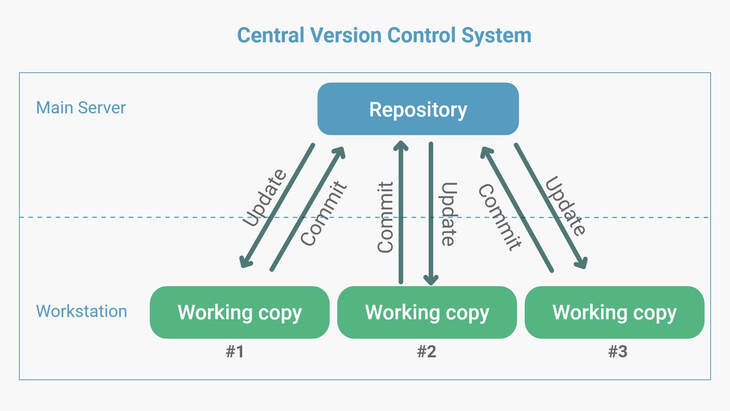
\includegraphics[width=\textwidth]{centralized-version-control-system-structure}
    \caption{Centralized Version Control System}
    \label{fig:cvcs-structure}
\end{figure}
% ==============================================================================
\subsection{Distributed Version Control Systems (DVCS)}
% TODO: Explain distributed VCS
% There are many advantages to using a distributed version control system (DVCS) over a centralized version control system (CVCS). DVCS is designed to work in two ways: it keeps the entire file history on each device locally and can also sync local modifications the user made with the server again when necessary so that the modifications can be shared with the whole team. In DVCS, the developers can work with different groups of people in different ways working on the same project. As well as any repository can be cloned, and, from a conceptual point of view, no repository is more significant than any other.
% In practice, the development team will organize the repositories in the hierarchy and at least one of the repositories will be marked as the central repository. To provide a new method for versioning software artifacts, several Distributed Version Control Systems emerged in the software field, such as Mercurial, Git, and Bazaar. These tools have been adopted by many Open Source Software (OSS) projects.
% The operations in DVCS are much faster than operations in CVCS because they are local. DVCS is considered to be the future of version control systems because it is suited for huge projects with more independent developers, and provides important advantages by allowing users to work and use a complete version control feature set even when there is no network connection. DVCS allows for version control of modifications done locally, allowing early drafts of work to be revised without requiring it to be released to others.
% There are many advantages to using DVCS: flexibility, hosting services like Github, availability, it is very fast due to its local nature to the majority of operations, it doesn’t require access to remote servers, and branching and merging can be done very easily in DVCS. Collaboration between team members and allow individual developers to be servers or clients are the most important features offer by version control systems, so developers can work on source code without being connected to a central or remote repository.
% There are some challenges introduced by DVCS: it lacks an understandable version numbering system, where there is no centralized versioning server, and uses hash modifications or a unique GUID. So, the lack of a central server makes system backup so difficult. The two most popular complaints about the disadvantages of DVCS are that: pessimistic locks are not available, and they have weak tools for binary.
% The reasons for the transition from centralized to decentralized version Control Systems are the ability to work offline and the ability to work incrementally. The ability of developers to made several roles, such as developing a new task or fixing errors, and the ability to do exploratory coding efficiently.
% TODO: OR
% ==============================================================================
Distributed Version Control Systems (DVCS) were created to overcome the limitations of Centralized Version Control Systems (CVCS), which enable branching and merging, avoid local VCS operations and allow developers collaboration. Due to the limitations associated with using a centralized version control system, Open Source Software (OSS) projects today largely adopt DVCS.

DVCS is designed to work in two ways as it keeps entire file histories locally on each device but can also sync local modifications made by users with servers again when necessary so that these modifications can be shared with everyone else. In DVCS developers are able to work separately or together but working on the same project as they have access to all repositories needed for their task; any repository can be cloned from another one so there's no more important repository than others.

To provide a new way for versioning software artifacts several Distributed Version Control Systems emerged in the software field such as \lstinline{Mercurial}, \lstinline{Git}, \lstinline{Bazaar}, etc. These tools have been adopted by many Open Source Software (OSS). The operations in DVCS are much faster than those found in CVSS because they're done locally while CVSS operations require remote connection; some consider that distributed systems will soon replace centralized ones because they suit bigger projects with more independent developers who want full functionality even without network connection available, offer advantages like earlier drafts of your work being saved without requiring you releasing them publicly or sharing them with other people etc.

Three major advantages offered by use of DVSs include flexibility availability which is related solely to its ability not needing access remotely servers for most operation types plus it's very fast due to its locality-based nature--most actions only need occur at one location unlike CVSCS versions where changes must travel through an often slower internet link before reaching their destination; branching merging is easy when working within DVSs due both high level abstraction language features provided but also lack requirement that user has knowledge about how specific models like Subversion operates making this process easier then would otherwise be possible under traditional model; collaboration between members/individual developer vs server/client differences make up most important feature offered by VSCs since team member may work on source code regardless whether connected centrally or remotely--this allows individual developer do exploratory coding efficiently too.

There are challenges introduced by use if DVSs including system backup being difficult cause lack central server makes creating backup virtually impossible meanwhile Pessimistic Locks aren't available either nor does present day software offer good support for binary files. Reasons why transition was made from centralized systems towards decentralized ones: offline capability enabling development portion done independently while maintaining integration into main branch + incremental capabilities providing greater efficiency during exploratory coding efforts.

\begin{figure}[h]
    \centering
    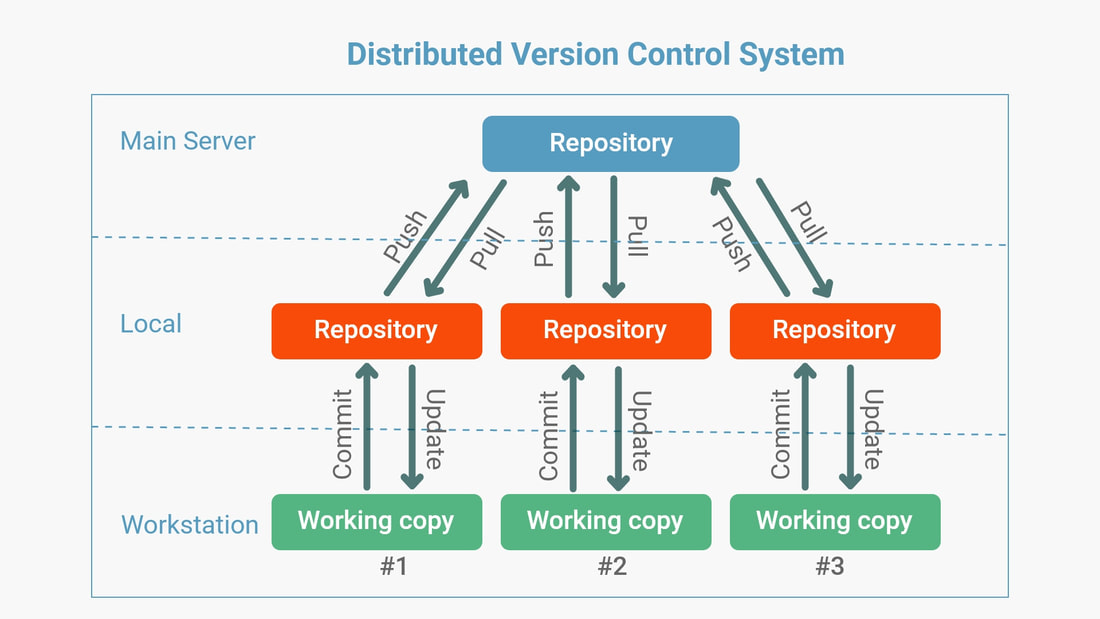
\includegraphics[width=\textwidth]{distributed-version-control-system-structure}
    \caption{Distributed Version Control System}
    \label{fig:dvcs-structure}
\end{figure}
% ==============================================================================
\section{Existing Version Control Systems}
\subsection{Local Version Control Systems}
Early VCS were intended to track changes for individual files and checked-out files could only be edited locally by one user at a time. They were built on the assumption that all users would log into the same shared Unix host with their own accounts. As you can imagine, these early systems made it easier for small teams to revisit code states from various points in history.
\subsubsection{Source Code Control System (SCCS)}
% TODO: Explain SCCS
SCCS was released in 1972, and it is one of the first successful VCS tools. It was written by Marc Rochkind at Bell Labs, who wanted to solve the problem of tracking file revisions. The tool made it significantly easier to track down bugs introduced into a program. SCCS is worth understanding at a basic level because it helped set up modern VCS tools that developers use today.
\paragraph{Architecture}
% TODO: Rewrite this section
Much like modern VCS tools, SCCS has a set of commands that allow developers to work with versioning of files. The basic command functionality are:
\begin{itemize}
    \item Check in files to track their history.
    \item Check out specific file versions for review.
    \item Check out specific file versions for editing.
    \item Check in new file versions with comments explaining the changes.
    \item Revert changes made to a checked out file.
    \item Basic branching and merging of changes.
    \item Print a log of a file's version history.
\end{itemize}
A special type of file called a \lstinline{s-file} or a \lstinline{history file} is created when a file is tracked by SCCS. This file is named with the original filename prefixed with a \lstinline{s.}, and is stored in a subdirectory called \lstinline{SCCS}.

So a file called \lstinline{test.txt} would get a history file created in the \lstinline{./SCCS/} directory with a name of \lstinline{s.test.txt}. When created, the \lstinline{s-file} contains the original file contents, a header that contains the file's version number, and some other metadata. There are also checksums stored in the \lstinline{s-file} that are used to verify the integrity of the file (i.e. to make sure that the file has not been tampered with). The \lstinline{s-file} content is not encoded or compressed in any way, which is a clear difference from modern VCS tools.

% TODO: Rewrite this section
% ==============================================================================
Since the content of the original file is now stored in the history file, it can be retrieved into the working directory for review, compilation, or editing. Further changes made to the file such as line additions, modifications, and removals can be checked back into the history file, which increments its revision number.

Subsequent SCCS checkins only store only the deltas or changes to a file as opposed to the entire file content each time. This decreases the size of the history file. Each time a checkin is made, the delta is stored in a structure known as a delta table inside the history file. As previously mentioned, the actual file content is more or less copied verbatim, with special control sequences for marking the start and end of sections of added and removed content. Since SCCS history files don't use compression, they are typically larger in size that the actual file being tracked. SCCS uses a delta method known as interleaved deltas. This is beneficial since it allows constant-time checkouts regardless of how old the checked out revision is - i.e. older revisions don't take longer to checkout than newer revisions.

One important thing to note is that all files are tracked and checked in separately in SCCS. There is no way to checkin changes to multiple files as a part of one atomic unit - like a commit in Git. Each tracked file has a corresponding history file which stores its revision history. In general, this means that the version numbers of different files in a project will not usually match each other. However, matching revision numbers can be achieved by editing every file in the project at once (even if not all of the files have real changes) and checking them all at one time. This will increment the revision number for all the files to keep them consistent, but note that this is NOT the same as including multiple files in a single commit like in Git. In SCCS, this makes an individual checkin in each history file, as opposed to one big commit including all the changes at once.

When a file is checked out for editing in SCCS, a lock is placed on the file so it cannot be edited by anyone else. This prevents changes from being overwritten by other users, but also limits development since only one user can work with a given file at a time.

SCCS has support for branches that can store sequences of changes within a specific file. Branches can be merged back in with the original versions or merged with other branched versions of the same parent.

% TODO: Restructure this section
\paragraph{Basic Commands}

Below is a list of the most common SCCS commands.

\lstinline{sccs create <filename.ext>} - Check in a new file to SCCS and create a new history file for it (in the \lstinline{./SCCS/} directory by default).

\lstinline{sccs get <filename.ext>} - Check out a file from from its corresponding history file and place it in the working directory in readonly mode.

\lstinline{sccs edit <filename.ext>} - Check out a file from the corresponding history file for editing. Locks the history file so no other users can modify it.

\lstinline{sccs delta <filename.ext>} - Check in the modifications to the specified file. Will prompt for a comment, store the changes in the history file, and remove the lock.

\lstinline{sccs prt <filename.ext>} - Display the revision log for a tracked file.

\lstinline{sccs diffs <filename.ext>} - Display the differences between the current working copy of a file and the state of the file when it was checked out.

% ==============================================================================
\subsubsection{Revision Control System (RCS)}
% TODO: Rewrite this section
% ==============================================================================
% TODO: Explain RCS
RCS was released in 1982, and it is another early VCS tool. It was written in C by Walter Tichy as an alternative to SCCS, which was still closed source at the time. RCS was released under the GNU General Public License, which allowed it to be used in open source projects.

"RCS manages revisions of text documents, in particular source programs, documentation, and test data. It automates the storing, retrieval, logging, and identification of revisions." - Walter Tichy
\paragraph{Architecture}
RCS shares many traits with its predecessor, including:
\begin{itemize}
    \item Handling revisions on a file-by-file basis.
    \item Changes across multiple files can't be grouped together into an atomic commit.
    \item Tracked files are intended to be modified by one user at a time.
    \item No network functionality.
    \item Revisions for each tracked file are stored in a corresponding history file.
    \item Basic branching and merging of revisions within individual files.
\end{itemize}
When a file is set checked into RCS for the first time, a corresponding history file is created for it in the local \lstinline{./RCS/} directory. This file is postfixed with a \lstinline{,v} so a file named \lstinline{test.txt} would be tracked by a file called \lstinline{test.txt,v}.

RCS uses a \lstinline{reverse-delta} scheme for storing file changes. When a file is checked in, a full snapshot of the file's content is stored in the history file. When the file is modified and checked in again, a delta is calculated based off of the existing history file content. The old snapshot is discarded and the new one is saved, along with the delta to get back to the older state.

This is called \lstinline{reverse-delta} since to check out an older revision, RCS starts with the newest version of the file and applies consecutive deltas until the older revision is reached. This method allows for very quick checkouts of current revisions since the full snapshot of the current revision is always available. However, the older the checkout revision, the longer the checkout takes since an increasing number of deltas need to be calculated against the current snapshot.

This is not the case with SCCS which takes the same amount of time to fetch any revision. In addition, no checksum is stored in RCS history files so file integrity cannot be ensured.

% TODO: List RCS commands
\paragraph{Basic Commands}

Below is a list of the most common RCS commands.

% ==============================================================================
\subsection{Centralized Version Control Systems}
Version control technology continued to evolve, leading to centralized repositories that contained the 'official' versions of their projects. This was good progress, since it allowed multiple users to checkout and work with the code at the same time as well as making commits back into this central repository. Furthermore, network access was required for people who wanted to commit changes they had made locally.
\subsubsection{Concurrent Versions System (CVS)}
Concurrent Versions System (CVS) was developed in by Dick Grune in 1986, it is also written in C. It was created with the goal of adding a networking element to version control. CVS became the first widely used VCS tool that allowed multiple users to work on the same project at the same time from different locations. This kicked off the second generation of VCS tools, allowing geographically dispersed development teams to work together on the same project.
\paragraph{Architecture}
CVS operates as a frontend for RCS - it provides a set of commands to interact with files in a project, but uses the RCS history file format and commands behind the scenes.

This meant that for the first time in history, multiple developers could check out and work on the same files simultaneously. It did this by utalising a centralized repository model.

% TODO: Rewrite this section
% ==============================================================================
The first step is to set up a centralized repository on a remote server using CVS. Projects can then be imported into the repository. When a project is imported into CVS, each file is converted into a \lstinline{,v} history file and stored in a central directory known as a \lstinline{module}. The repository generally lives on a remote server which is accessible over a local network or the Internet.

A developer checks out a copy the module which is copied to a working directory on their local machine. No files are locked in this process so there is no limit to the number of developers that can check out the module at one time. Developers can modify their checked out files and commit their changes as needed. If a developer commits a change, other developers will need to update their working copies via a (usually) automated merge process before committing their changes. Occasionally merge conflicts will need to be manually resolved before the commit can be made. CVS also provides the ability to create and merge branches.
% ==============================================================================

% TODO: List CVS commands
\paragraph{Basic Commands}

Below is a list of the most common CVS commands.

% ==============================================================================
\subsubsection{Apache Subversion (SVN)}
Subversion (SVN) was developed by CollabNet in 2000 and is now maintained by the Apache Software Foundation. It is written in C and was designed to be a more robust centralized solution than CVS.
\paragraph{Architecture}
% TODO: Rewrite this section
% ==============================================================================
Similar to CVS, SVN uses a centralized repository model. Remote users must have a working network connection to commit their changes to the central repository.

Subversion introduced the functionality of atomic commits which ensured that a commit would either fully succeed, or be completely abandoned if an issue occurred.

In CVS, if a commit operation failed midway, for example due to a network outage, the repository could be left in a corrupted and inconsistent state. Furthermore, a commit or revision in Subversion can include multiple files and directories. This is important since it allows users to track sets of related changes together as a grouped unit, instead of the past storage models that track changes separately for each file.

The current storage model that Subversion uses for tracked files is called \lstinline{FSFS} or \lstinline{File System atop the File System}. This name was chosen since it creates its database structure using a file and directory structure that match the operating system filesystem it is running on. The unique feature of the Subversion filesystem is that it is designed to track not only the files and the directories it contains, but the different versions of these files and directories and they change over time. It is a filesystem with an added time dimension. In addition, folders are first class citizens in Subversion. Empty folders can be committed in Subversion, whereas in the rest (even Git) empty folders are unnoticed.

When a Subversion repository is created, a (nearly) empty database of files and folders is created as a part of it. A directory called \lstinline{db/revs} is created in which all revision tracking information for the checked-in (committed) files is stored. Each commit (which can include changes to multiple files) is stored in a new file in the \lstinline{revs} directory and is named with a sequential numeric identifier starting with 1. When a file is committed for the first time, its full content is stored. Future commits of the same file will store only the changes - also called the \lstinline{diffs} or \lstinline{deltas} - in order to conserve space. In addition, the deltas are compressed using \lstinline{lz4} or \lstinline{zlib} compression algorithms to further reduce their size.

By default, this is actually only true to a point. Although storing file deltas instead of the whole file each time does save on storage space, it adds time to checkout and commit operations since all the deltas need to be strung together in order to recreate the current state of the file. For this reason, by default Subversion stores up to 1023 deltas per file before storing a new full copy of the file. This achieves a nice balance of both storage and speed.

SVN does not use a conventional branching and tagging system. A normal Subversion repository layout is to have three folders in the root:
\begin{itemize}
    \item \lstinline{trunk/}
    \item \lstinline{branches/}
    \item \lstinline{tags/}
\end{itemize}
The \lstinline{trunk/} folder is used for the production version of the application.
The \lstinline{branches/} folder is used to store subfolders that correspond to individual branches.
The \lstinline{tags/} folder is used to store tags which represent specific (usually significant) project revisions.
% ==============================================================================

% TODO: List SVN commands
\paragraph{Basic Commands}

Below is a list of the most common SVN commands.

% ==============================================================================
\subsubsection{Perforce Helix Core}
% Perforce is a centralized VCS that was developed by Perforce Software in 1995. Perforce is a commercial VCS that is used by many large companies, such as Google, Adobe and IBM. It is still one of the largest version control systems in use today.
% TODO: Rewrite this section
% ==============================================================================
Perforce Helix Core is a proprietary VCS created, owned, and maintained by Perforce Software, Inc. It is typically set up using a centralized model although it does offer a distributed model option. It is written in C and C++, and was initially released in 1995. It is primarily used by large companies that track and store a lot of content using large binary files, as is the case in the video game development industry. Although Helix Core is typically cost prohibitive for smaller projects, Perforce offers a free version for teams of up to 5 developers.
\paragraph{Architecture}
Perforce Helix Core is set up as a server/client model. The server is a process called \lstinline{p4d} which waits and listens for incoming client connections on a designated port, typically port 1666. The client is a process called \lstinline{p4} which comes in both command-line and GUI flavors. Users run the \lstinline{p4} client to connect to the server and issue commands to it. Support is available for various programming language APIs, including Python and Java. This allows automated issuance and processing of Helix Core commands via scripts. Integrations are also available for IDEs like Eclipse and Visual Studio, allowing users to work with version control from within those tools.

The Helix Core Server manages repositories referred to as depots, which store files in directory trees, not unlike Subversion (SVN). Clients can checkout sets of files and directories from the depots into local copies called \textbf{workspaces}. The atomic unit used to group and track changes in Helix Core depots is called the \textbf{changelist}. Changelists are similar to Git commits. Helix Core implements two similar forms of branching - \textbf{branches} and \textbf{streams}. Branches are conceptually similar to what we are used to - separate lines of development history. A stream is a branch with added functionality that Helix Core uses to provide recommendations on best merging practices throughout the development process.

When a file is added for tracking, Helix Core classifies it using a \textbf{file type} label. The two most commonly used file types are text and binary. For binary files, the entire file content is stored each time the file is stored. This is a common VCS tactic for dealing with binary files which are not amenable to the normal merge process, since manual conflict resolution is usually not possible.

For text files, only the deltas (changes between revisions) are stored. Text file history and deltas are stored using the RCS (Revision Control System) format, which tracks each file in a corresponding \lstinline{,v} file in the server depot. This is similar to CVS, which also leverages RCS file formats for preserving revision history. Files are often compressed using gzip when added to the depot and decompressed when synced back to the workspace.

% TODO: Add annotated comment
% It is suprising that such a longstanding proprietary software like Perforce would base itself on a seemingly antiquated and open-source root like RCS, especially for such an essential component (its delta and history file backend)...

% TODO: List Perforce commands
\paragraph{Basic Commands}

Below is a list of the most common Perforce commands.

% ==============================================================================
\subsection{Distributed Version Control Systems}
In a distributed version control system, all copies of the repository are created equal - there is no central copy of the repository. This design principle encourages commits, branches and merges to be created locally without network access and pushed to other repositories as needed.
\subsubsection{Git}
% Git is a distributed VCS that was developed by Linus Torvalds in 2005. Git is a free and open source VCS that is used by many large companies, such as Google, Facebook and Twitter. It is one of the most popular version control systems in use today.
% TODO: Rewrite this section
% ==============================================================================
Git was created in 2005 by Linus Torvalds (also the creator of Linux) and is written primarily in C combined with some shell scripts. It is widely considered the best VCS tool due to its features, flexibility, and speed. Linus Torvalds originally wrote it for the Linux codebase and it has grown to become the most popular VCS in use today.

"You can do a lot of things with Git, and many of the rules of what you should do are not so much technical limitations but are about what works well when working together with other people. So Git is a very powerful set of tools, and that can not only be overwhelming at first, it also means that you can often do the same (or similar) things different ways, and they all 'work.'" - Linus Torvalds

Git repositories are commonly hosted on local servers as well as cloud services. Git forms the backbone of a broad set of DevOps tools available from popular service providers including GitHub, BitBucket, GitLab, and many others.
\paragraph{Architecture}
Git is a distributed VCS. This means that no copy of the repository needs to be designated as the centralized copy - all copies are created equal. This is in stark contrast to the second generation VCS which rely on a centralized copy for users to checkin and checkout from.

What this means is that developers and coding partners can share changes with each other directly before merging their changes into an official branch. This allows team collaboration to take on a flexible distributed workflow, if desired.

Furthermore, developers can commit their changes to their local copy of the repository without any other repositories knowing about it. This means that commits can be made without any network or Internet connection. Developers can work locally offline until they are ready to share their work with others. At that point, the changes can be pushed to other repositories for review, testing, or deployment.

When a file is added for tracking with Git, it is compressed using the \lstinline{zlib} compression algorithm. The result is hashed using a SHA-1 hash function. This yields a unique hash value that corresponds specifically to the content in that file. Git stores this in an \lstinline{object database} which is located in the hidden \lstinline{.git/objects} folder.

The name of the file is the generated hash value, and the file contains the compressed content. These files are called Git blobs and are created each time a new file (or changed version of an existing file) are added to the repository.

"The object database is literally just a content-addressable collection of objects. All objects are named by their content, which is approximated by the SHA1 hash of the object itself. Objects may refer to other objects (by referencing their SHA1 hash), and so you can build up a hierarchy of objects." - Linus Torvalds

Git implements a \lstinline{staging index} which acts as an intermediate area for changes that are getting ready to be committed. As new changes are staged for commit, their compressed contents are referenced in a special index file - which takes the form of a \lstinline{tree} object. A \lstinline{tree} is a Git object that connects blob objects to their real file names, file permissions and links to other trees, and in this way represents the state of a particular set of files and directories. Once all related changes are staged for commit, the index tree can be committed to the repository, which creates a \lstinline{commit} object in the Git object database.

A commit references the head tree for a particular revision as well as the commit author, email address, date, and a descriptive commit message. Each commit also stores a reference to its parent commit(s) and so over time a history of project development is established.

As mentioned, all Git objects - blobs, trees, and commits - are compressed, hashed, and stored in the object database based on their hash value. These are called \lstinline{loose objects}. At this point no diffs have been utilized to save space which makes Git very fast since the full content of each file revision is accessible as a loose object.

However, certain operations such as pushing commits to a remote repository, storing too many objects, or manually running Git's garbage collection command can cause Git to repackage the objects into \lstinline{pack files}. In the packing process, reverse diffs are taken and compressed to eliminate redundant content and reduce size. This process results in \lstinline{.pack} files containing the object content, each with a corresponding \lstinline{.idx} (or index) file containing a reference of the packed objects and their locations in the pack file.

These pack files are transferred over the network when branches are pushed to or pulled from remote repositories. When pulling or fetching branches, the pack files are unpacked to create the loose objects in the object repository.

\paragraph{Basic Commands}

\begin{itemize}
    \item \lstinline{git init} - Initialize a Git repository in the current directory (creates the hidden \lstinline{.git} folder and its contents).
    \item \lstinline{git clone <git-url>} - Download a copy of the Git repository at the specified URL.
    \item \lstinline{git add <filename.ext>} - Add an untracked file or changed file to the staging area (creates corresponding entries in the object database).
    \item \lstinline{git commit -m 'Commit message'} - Commit a set of changed files and folders along with a descriptive commit message.
    \item \lstinline{git status} - Show information related to the state of the working directory, current branch, untracked files, modified files, etc.
    \item \lstinline{git branch <new-branch>} - Create a new branch based on the current checked-out branch.
    \item \lstinline{git checkout <branch>} - Checkout the specified branch into the working directory.
    \item \lstinline{git merge <branch>} - Merge the specified branch into the current branch checked-out in the working directory.
    \item \lstinline{git pull} - Update the working copy by merging in committed changes that exist in the remote repository but not the working copy.
    \item \lstinline{git push} - Pack loose objects for local active branch commits into pack files and transfer to remote repository.
    \item \lstinline{git log} - Show the commit history and associated descriptive messages for the active branch.
    \item \lstinline{git stash} - Save all uncommitted changes in the working directory to a cache so that they can be retrieved later.
\end{itemize}

% ==============================================================================
\subsubsection{Mercurial}
% Mercurial is a distributed VCS that was developed by Matt Mackall in 2005. Mercurial was developed with the same goal as Git, to maintain the Linux kernal project.
% TODO: Rewrite this section
% ==============================================================================
Mercurial was created in 2005 by Matt Mackall and it is written in Python. It was also started with the goal of hosting the codebase for Linux, but Git was chosen instead. It is the second most popular distributed VCS after Git, but is used far less often.
\paragraph{Architecture}
Like Git, Mercurial is a distributed version control system that allows any number of developers to work with their own copy of a project independently from others.

Mercurial leverages many of the same technologies as Git, such as compression and SHA-1 hashing, but does so in different ways.

When a new file is committed for tracking in Mercurial, a corresponding \lstinline{revlog} file is created for it in the hidden directory \lstinline{.hg/store/data/}. You can think of a \lstinline{revlog} (or revision log) file as a modernized version of the \lstinline{history files} used by the older VCS like CVS, RCS, and SCCS.

Unlike Git, which creates a new blob for every version of every staged file, Mercurial simply creates a new entry in the revlog for that file. To conserve space, each new entry only contains the delta (changes) from the previous version. Once a threshold number of deltas is reached, a full snapshot of the file is stored again.

This reduces the lookup time when applying many deltas to reconstruct a particular file revision.

These file revlogs are named to match the files that they track, but are postfixed with \lstinline{.i} and \lstinline{.d} extensions. The \lstinline{.d} files contained the compressed delta content. The \lstinline{.i} files are used as indexes to quickly track down different revisions inside the \lstinline{.d} files. For small files with low numbers of revisions, both the indexes and content are stored in \lstinline{.i} files. Revlog file entries are compressed for performance and hashed for identification. The hash values are referred to as \lstinline{nodeids}.

Whenever a new commit is made, Mercurial tracks the all file revisions in that commit in something called the \lstinline{manifest}. The manifest is also a revlog file - it stores entries that correspond to particular states of the repository.

However, instead of storing individual file content like the file revlogs, the manifest stores a list of filenames and nodeids that specify which file revision entries exist in each revision of the project. These manifest entries are also compressed and hashed. The hash values are again referred to as \lstinline{nodeids}.

Lastly, Mercurial uses one more type of revlog called a \lstinline{changelog}. The changelog contains a list of entries that associate each commit with the following information:
\begin{itemize}
    \item Manifest nodeid - Identifies the full set of file revisions that exist at a particular time.
    \item Parent commit nodeid(s) - This allows Mercurial to establish a timeline or branch of project history. One or two parent ID's are stored depending on the type of commit (normal vs merge).
    \item Commit author
    \item Commit date
\end{itemize}
Each changelog entry also generates a hash known as its \lstinline{nodeid}.

\paragraph{Basic Commands}
\begin{itemize}
    \item \lstinline{hg init} - Initialize the current directory as a Mercurial repository (creates the hidden \lstinline{.hg} folder and its contents).
    \item \lstinline{hg clone <hg-url>} - Download a copy of the Mercurial repository at the specified URL.
    \item \lstinline{hg add <filename.ext>} - Add a new file for revision tracking.
    \item \lstinline{hg commit -m 'Commit message'} - Commit a set of changed files and folders along with a descriptive commit message.
    \item \lstinline{hg status} - Show information related to the state of the working directory, untracked files, modified files, etc.
    \item \lstinline{hg update <revision>} - Checkout the specified branch into the working directory.
    \item \lstinline{hg merge <branch>} - Merge the specified branch into the current branch checked out in the working directory.
    \item \lstinline{hg pull} - Download new revisions from remote repository but don't merge them into the working directory.
    \item \lstinline{hg push} - Transfer new revisions to remote repository.
    \item \lstinline{hg log} - Show the commit history and associated descriptive messages for the active branch.
\end{itemize}


% ==============================================================================
\subsubsection{BitKeeper}
% TODO: Explain BitKeeper
\paragraph{Advantages}
% TODO: Add advantages
\paragraph{Disadvantages}
% TODO: Add disadvantages
\subsubsection{Darcs Advanced Revision Control System (Darcs)}
% TODO: Explain Darcs
\paragraph{Advantages}
% TODO: Add advantages
\paragraph{Disadvantages}
% TODO: Add disadvantages
\subsubsection{Monotone}
% TODO: Explain Monotone
\paragraph{Advantages}
% TODO: Add advantages
\paragraph{Disadvantages}
% TODO: Add disadvantages
\subsubsection{Bazaar}
% TODO: Explain Bazaar
\paragraph{Advantages}
% TODO: Add advantages
\paragraph{Disadvantages}
% TODO: Add disadvantages
\subsubsection{Fossil}
% TODO: Explain Fossil
\paragraph{Advantages}
% TODO: Add advantages
\paragraph{Disadvantages}
% TODO: Add disadvantages
% ==============================================================================
\section{Summary of Key Features}
\subsection{Repositories}
% TODO: Explain repositories
\subsection{Commits}
% TODO: Explain commits
\subsection{Branching and Merging}
% TODO: Explain branching and merging
\subsection{Pulling and Pushing}
% TODO: Explain pulling and pushing

\newpage
\chapter{Design}
% TODO: Add design chapter
\newpage
\chapter{Implementation} % (30-40 pages)
\label{chap:implementation}

% Environment Setup - (1 page)
% File System Interaction - (1 page)

% Data Structures
% ---------------
% Implementing the data structures - (4 x 2 page)
% Testing the data structures - (4 x 1 page)

% Algorithms
% ---------------
% Implementing the algorithms
%  - Hashing - (2 x 1 page)
%  - Diffing - (2 x 3 page)
%  - Merging - (2 x 3 page)
% Testing the algorithms
%  - Hashing - (1 page)
%  - Diffing - (2.5 page)
%  - Merging - (2.5 page)

% Benchmarks
% ---------------
% Data Structures - (1 page)
% Algorithms - (3 page)


\newpage
\chapter{Evaluation} % (10-15 pages)
\label{chap:eval}

\section{Data Gathering}
\noindent
Before evaluating the performance benchmarks, we need to understand the format of the benchmark output and how to parse the output into usable data.

\subsection*{Benchmark Output}

\begin{lstlisting}[language=prolog]
goos: linux
goarch: amd64
pkg: search
BenchmarkDepthFirstSearch/revisions=200,dataSize=100-16         	  393714	      8504 ns/op	    4249 B/op	      15 allocs/op
BenchmarkDepthFirstSearch/revisions=200,dataSize=1000-16        	  419702	      8537 ns/op	    4256 B/op	      15 allocs/op
BenchmarkDepthFirstSearch/revisions=2000,dataSize=100-16        	   39650	     90070 ns/op	   47976 B/op	      68 allocs/op
BenchmarkDepthFirstSearch/revisions=2000,dataSize=1000-16       	   39520	     92031 ns/op	   48012 B/op	      68 allocs/op
\end{lstlisting}
\medskip

The first items printed in the benchmark output are the two core \lstinline{Go} environment variables, \lstinline{GOOS} (Operating System, e.g., \lstinline{linux}) and \lstinline{GOARCH} (CPU Architecture, e.g., \lstinline{amd64}), followed by the \lstinline{pkg} (package name) which contains the benchmark functions being executed. Finally, the remaining lines contain the individual benchmark results, containing the following columns\cite{andile_2023}:

\begin{enumerate}
    \item \textless\lstinline{Name of benchmark}\textgreater\ -- \textless\lstinline{Number of CPU cores}\textgreater\\The name of the benchmark function being executed, followed by the number of CPU cores used to execute the benchmark. This is useful for identifying the number of CPU cores used to execute the benchmark, as the number of CPU cores used is not explicitly stated in the benchmark output.
    \item \textless\lstinline{Number of iterations}\textgreater\\The number of iterations executed by the benchmark function to produce the average performance metrics.
    \item \textless\lstinline{Average number of nanoseconds per operation}\textgreater\\The average number of nanoseconds taken to execute a single operation of the benchmark function.
    \item \textless\lstinline{Average number of Bytes allocated per operation}\textgreater\\The average number of Bytes allocated to execute a single operation of the benchmark function.
    \item \textless\lstinline{Average number of memory allocations per operation}\textgreater\\The average number of memory allocations to execute a single operation of the benchmark function.
\end{enumerate}

\subsection*{Data Parsing}
A \lstinline{Python} script was employed to parse usable data from the \lstinline{Go} benchmark logs. The script leveraged regular expressions to identify and extract key performance metrics such as the number of iterations, time taken per operation (in nanoseconds), memory allocated per operation (in bytes), and the number of memory allocations per operation. This information was then stored in a CSV file format, facilitating easy data analysis and visualisation.

\begin{lstlisting}[language=python]
import csv
import re

benchmark_pattern = re.compile(
    r"Benchmark([\w_]+)/revisions=(\d+),dataSize=(\d+)-(\d+)
        \s+(\d+)\s+(\d+) ns/op\s+(\d+) B/op\s+(\d+) allocs/op"
)

csv_headers = [
    "benchmark_name",
    "num_revisions",
    "data_size",
    "num_cpus",
    "iterations",
    "ns_per_op",
    "bytes_per_op",
    "allocs_per_op",
]

for log_file, csv_file in log_files.items():
    with open(log_file, "r") as f:
        content = f.read()

    benchmarks = benchmark_pattern.findall(content)
    
    with open(csv_file, "w", newline="") as f:
        writer = csv.writer(f)
        writer.writerow(csv_headers)
        for benchmark in benchmarks:
            writer.writerow(benchmark)

\end{lstlisting}

\subsection*{Performance Metrics}
In order to compare the performance of the implemented algorithms and data structures, we considered the following key performance metrics:

\paragraph{Execution time \(ns\_per\_op\)}
The time taken per operation (in nanoseconds) was a primary factor in determining the efficiency of the algorithms. Lower execution times indicate better performance.

\paragraph{Memory usage \(bytes\_per\_op\)}
Memory allocated per operation (in bytes) was another crucial aspect to evaluate, as efficient algorithms should minimise memory consumption.

\paragraph{Memory allocations \(allocs\_per\_op\)}
The number of memory allocations per operation was also taken into account, as fewer allocations generally indicate a more optimised algorithm.

\section{Data Structures}

\subsection{Doubly Linked List}

\begin{table}[h]
    \centering
    \begin{tabular}{|r|r|r|r|r|}
        \hline
        \multicolumn{1}{|c|}{\textbf{num\_revisions}} & \multicolumn{1}{c|}{\textbf{data\_size}} & \multicolumn{1}{c|}{\textbf{ns\_per\_op}} & \multicolumn{1}{c|}{\textbf{bytes\_per\_op}} & \multicolumn{1}{c|}{\textbf{allocs\_per\_op}} \\ \hline
        200 Revs                                      & 100 byte/rev                             & 714030                                    & 35200                                        & 600                                           \\ \hline
        200 Revs                                      & 1000 byte/rev                            & 3989548                                   & 217604                                       & 600                                           \\ \hline
        200 Revs                                      & 10000 byte/rev                           & 36909724                                  & 2060860                                      & 600                                           \\ \hline
        2000 Revs                                     & 100 byte/rev                             & 10124801                                  & 352003                                       & 6000                                          \\ \hline
        2000 Revs                                     & 1000 byte/rev                            & 40641532                                  & 2176026                                      & 6000                                          \\ \hline
        2000 Revs                                     & 10000 byte/rev                           & 344262304                                 & 20608074                                     & 6000                                          \\ \hline
        20000 Revs                                    & 100 byte/rev                             & 455200208                                 & 3520027                                      & 60000                                         \\ \hline
        20000 Revs                                    & 1000 byte/rev                            & 759428984                                 & 21760746                                     & 60003                                         \\ \hline
        20000 Revs                                    & 10000 byte/rev                           & 3792506585                                & 206080096                                    & 60001                                         \\ \hline
    \end{tabular}
    \caption{Performance metrics for the Doubly Linked List implementation.}
    \label{tab:doubly-linked-list-benchmark-results}
\end{table}

\begin{figure}[H]
    \centering
    \begin{subfigure}[b]{0.8\textwidth}
        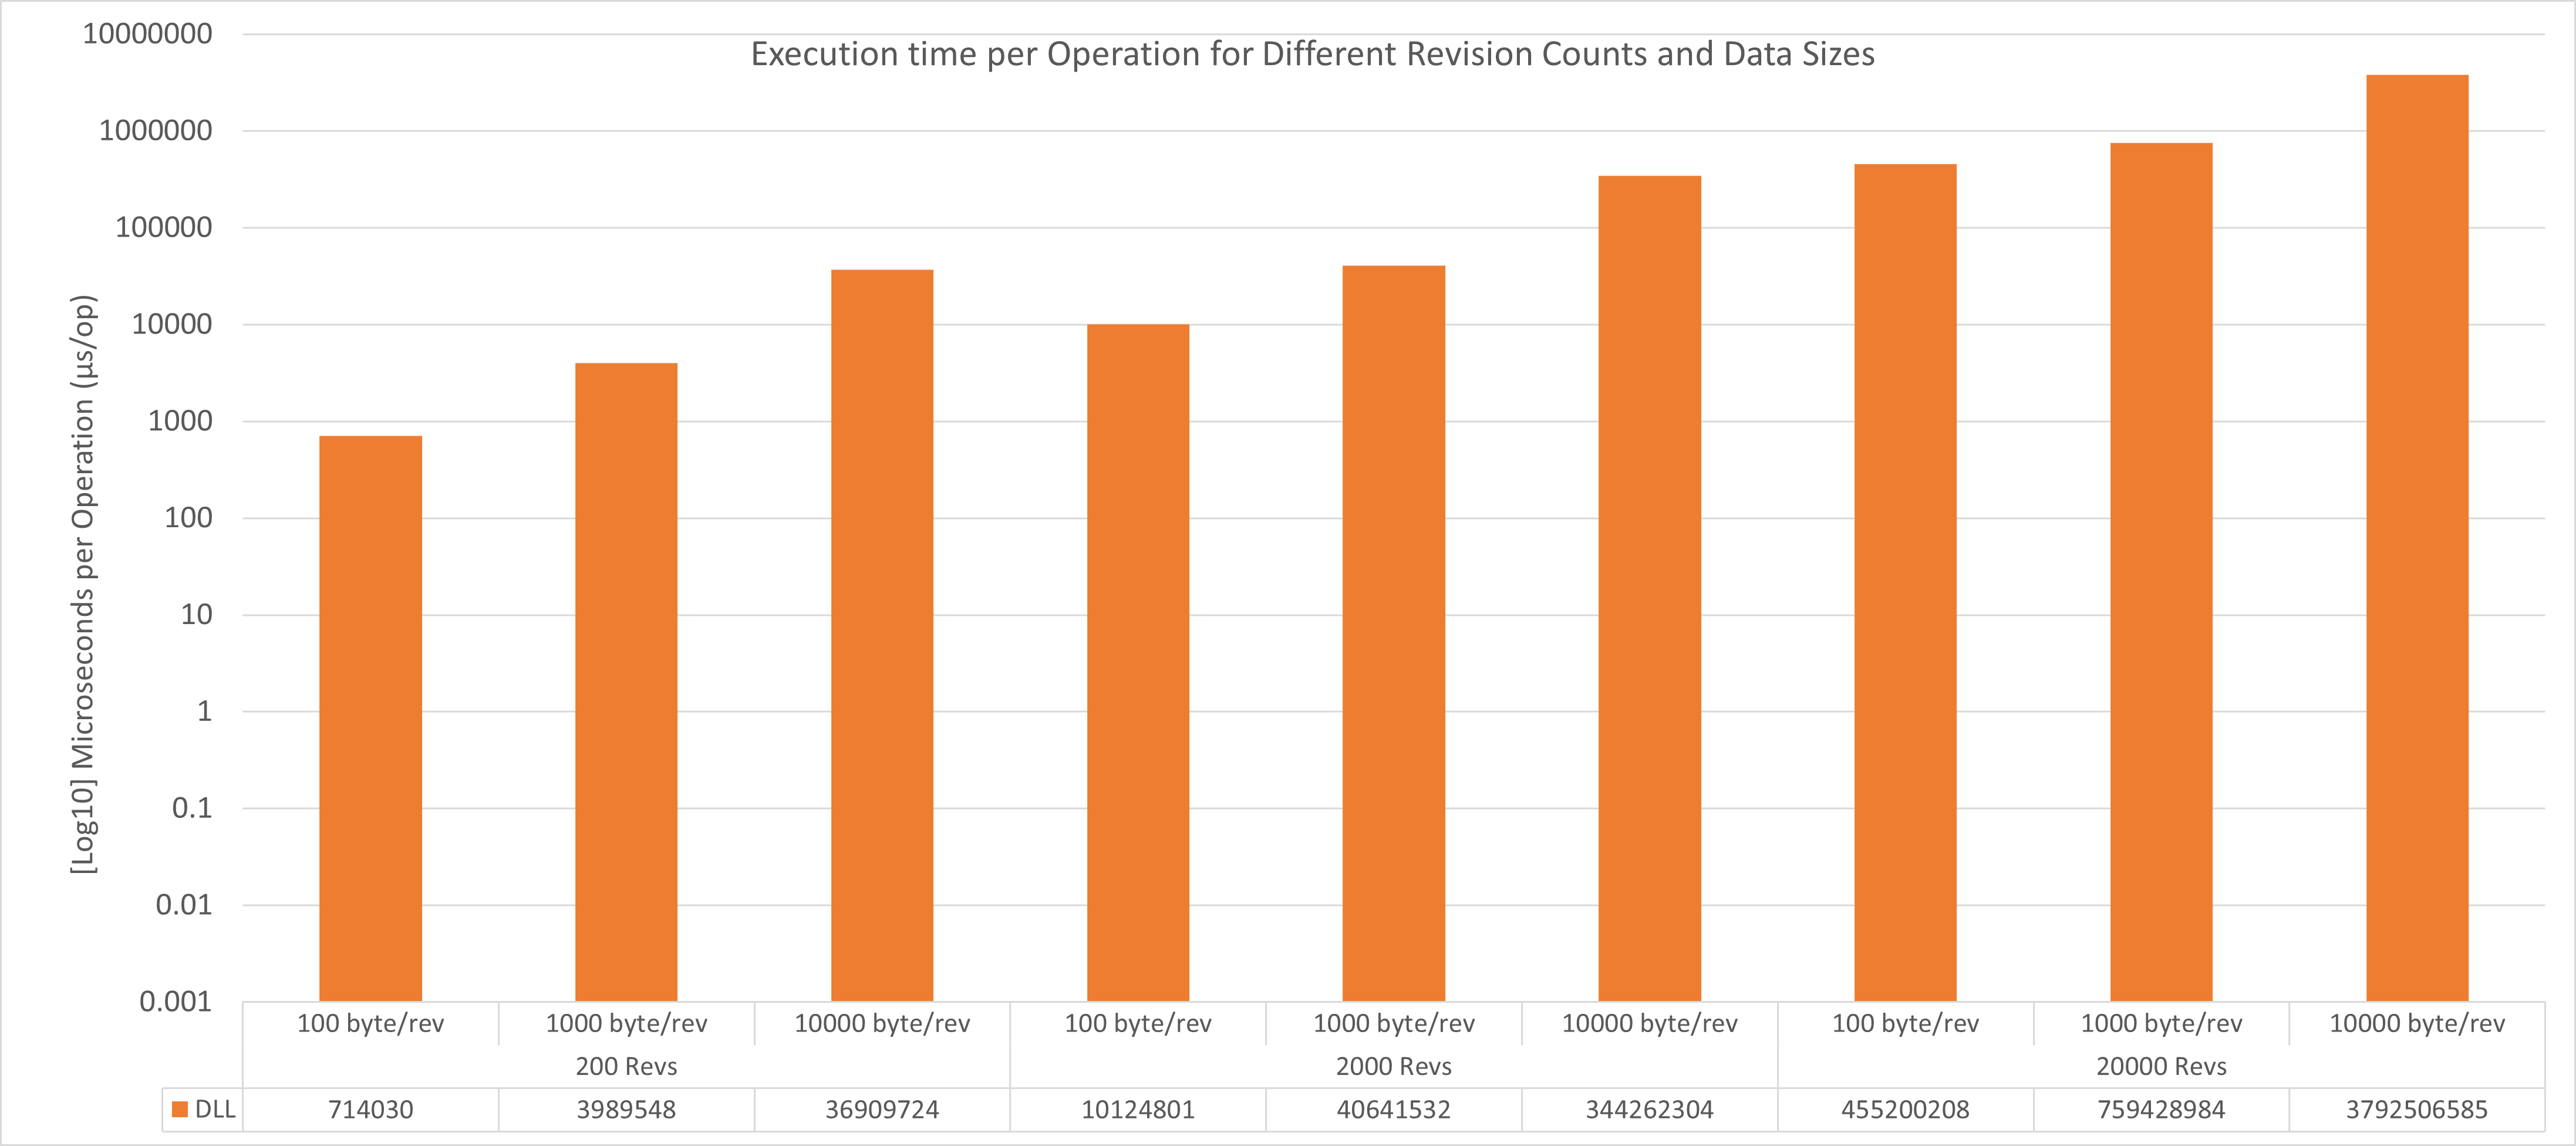
\includegraphics[width=1\linewidth]{charts/dll_ns_all.png}
        \caption{Execution Time}
        \label{fig:doubly-linked-list-execution-time}
    \end{subfigure}

    \begin{subfigure}[b]{0.8\textwidth}
        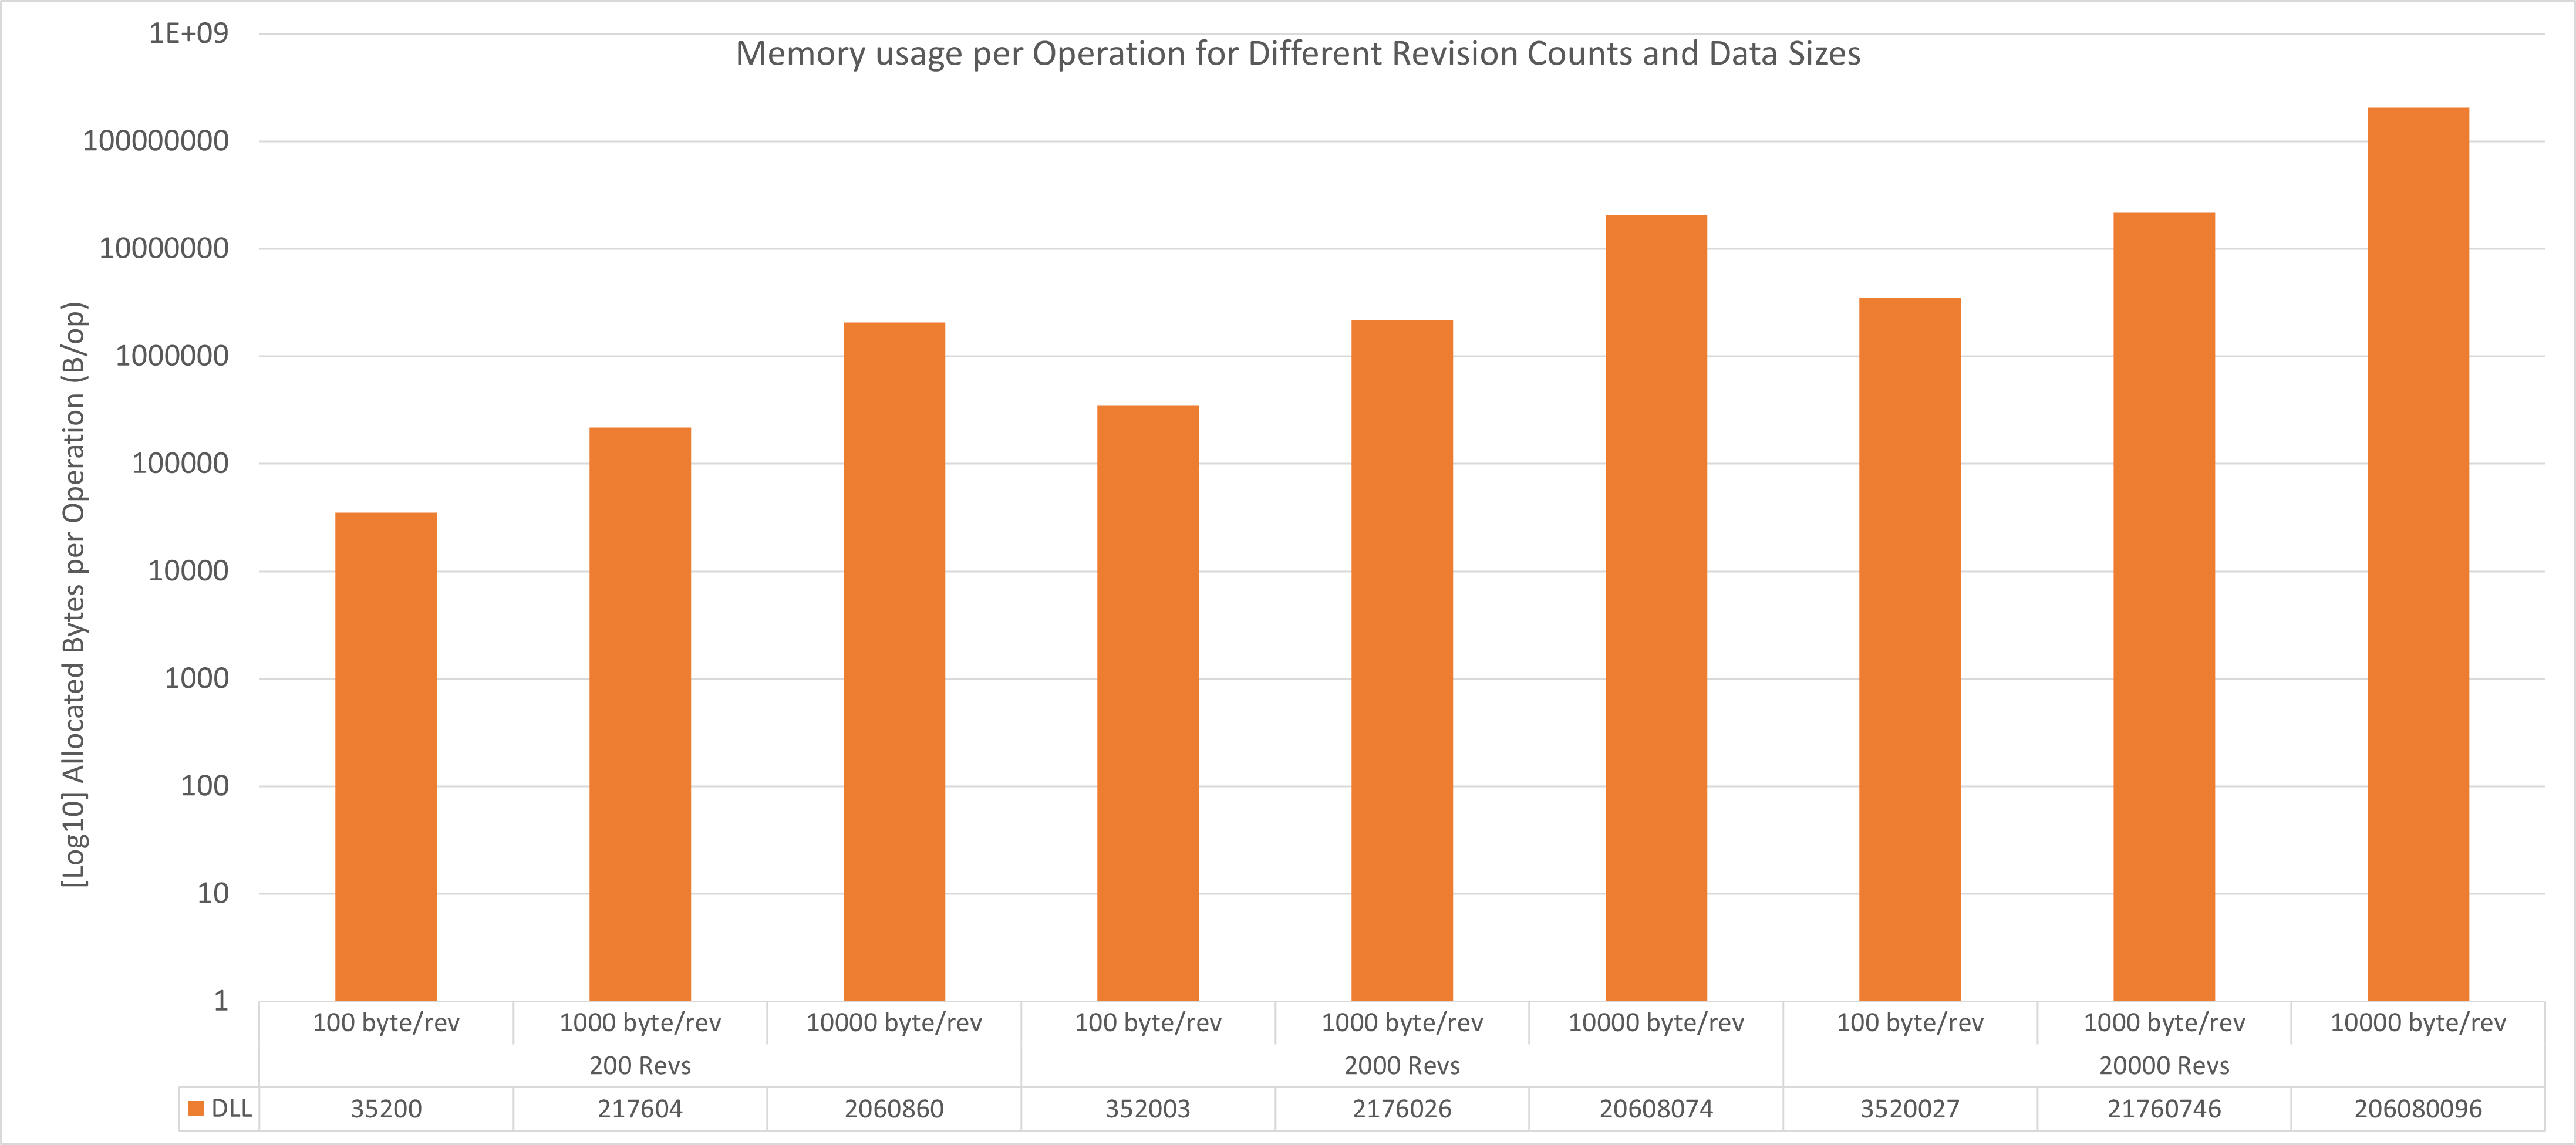
\includegraphics[width=1\linewidth]{charts/dll_bytes_all.png}
        \caption{Memory Usage}
        \label{fig:doubly-linked-list-memory-usage}
    \end{subfigure}

    \begin{subfigure}[b]{0.8\textwidth}
        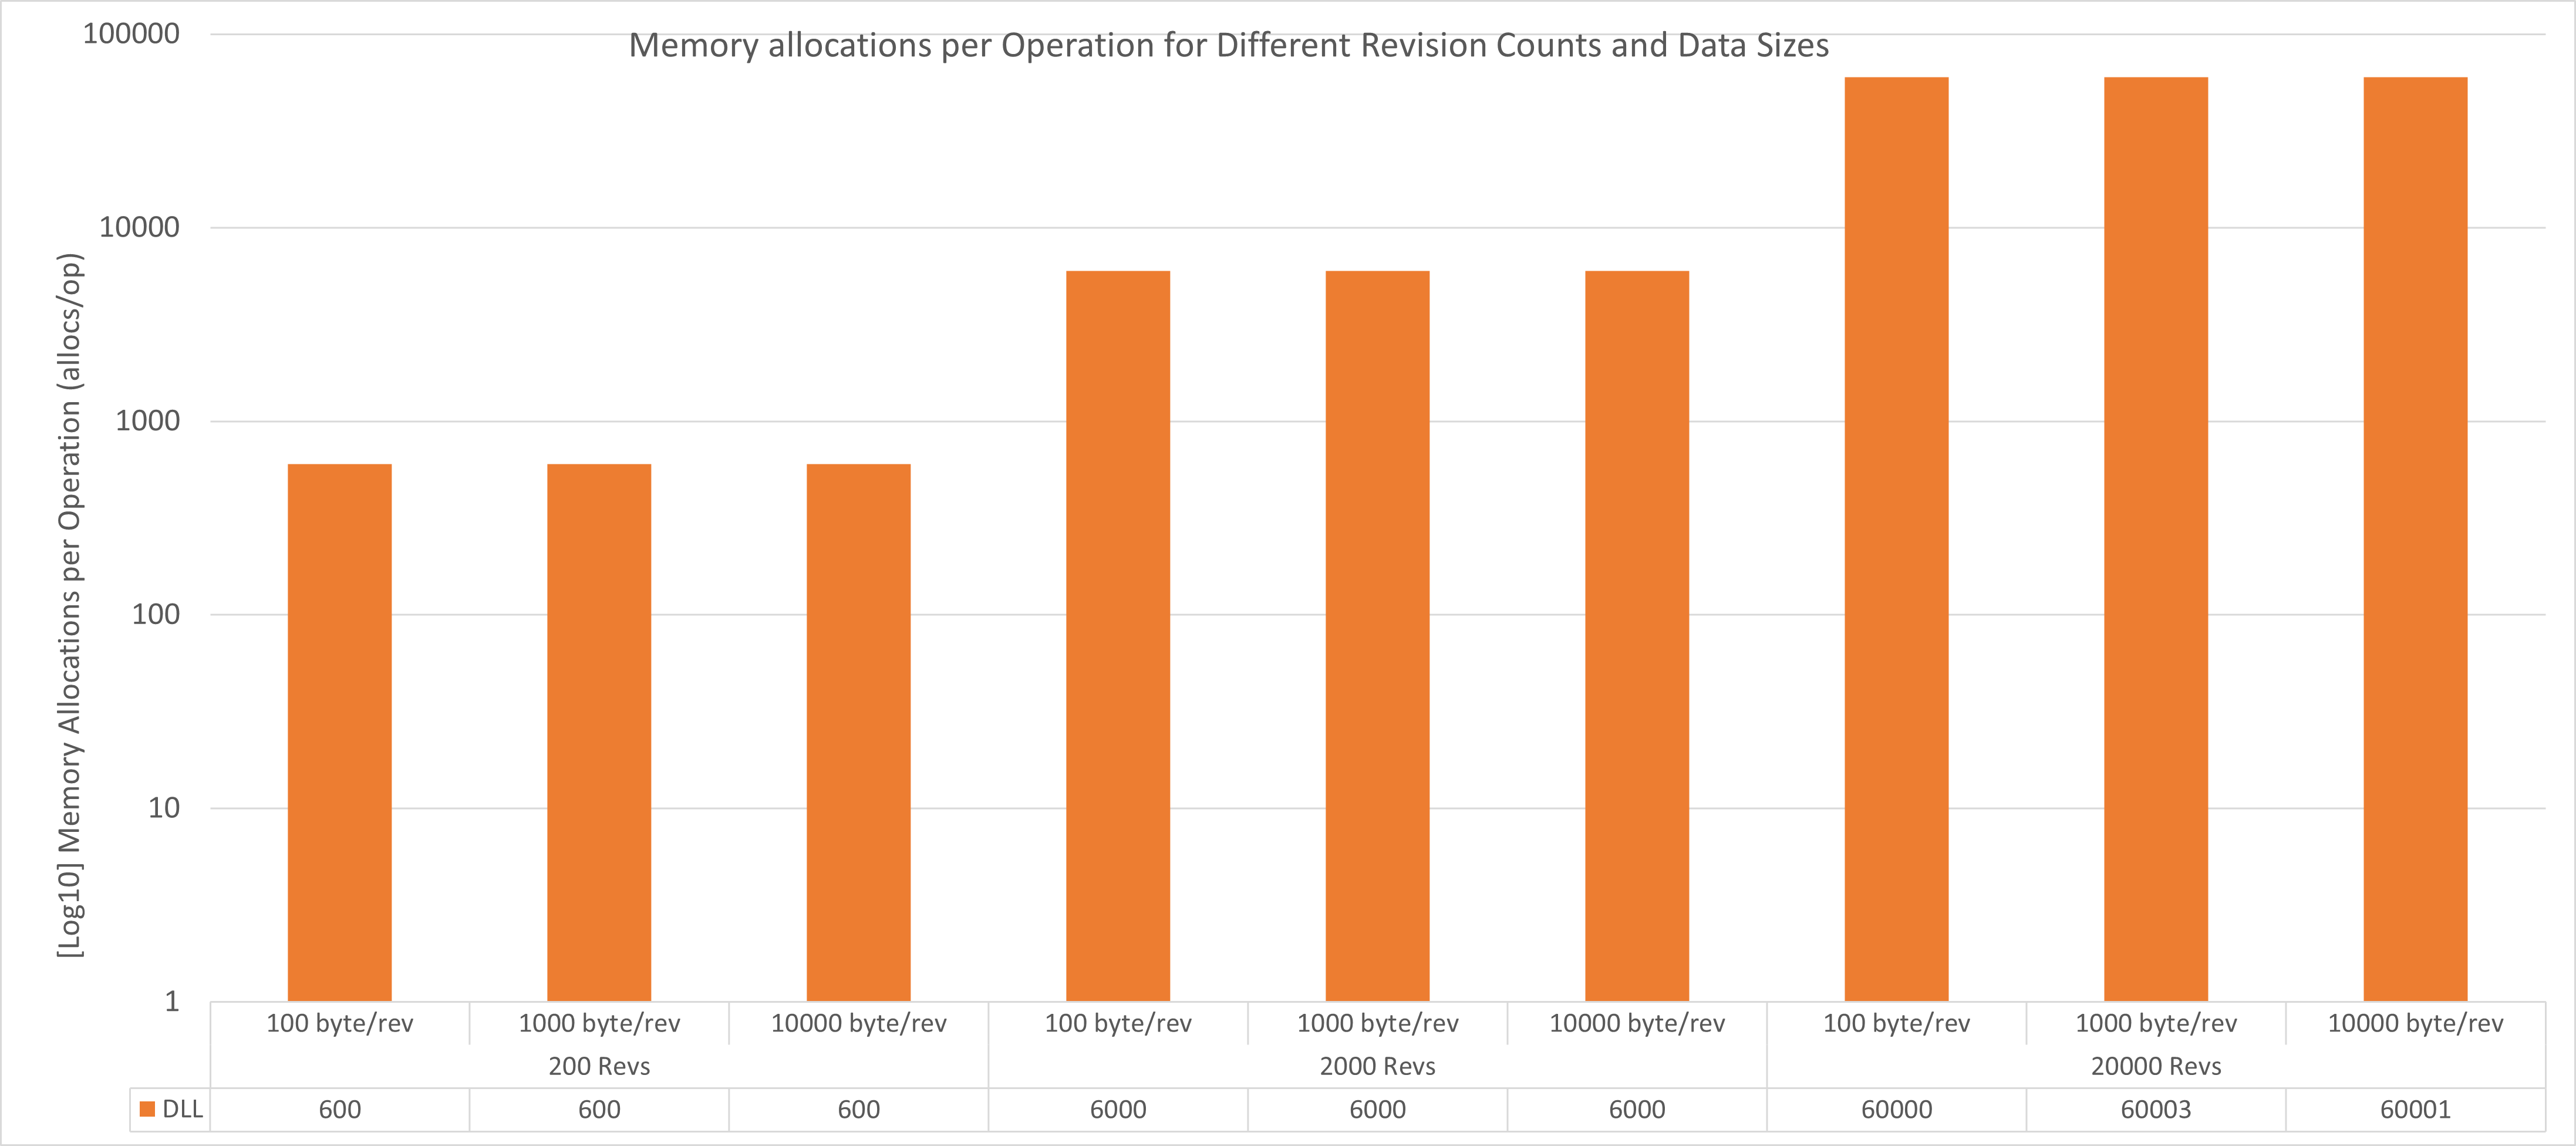
\includegraphics[width=1\linewidth]{charts/dll_allocs_all.png}
        \caption{Memory Allocations}
        \label{fig:doubly-linked-list-memory-allocations}
    \end{subfigure}

    \caption{Performance metrics for the Doubly Linked List implementation.}
    \label{fig:doubly-linked-list-performance-metrics}
\end{figure}

\subsection{Binary Search Tree}

\begin{table}[h]
    \centering
    \begin{tabular}{|r|r|r|r|r|}
        \hline
        \multicolumn{1}{|c|}{\textbf{num\_revisions}} & \multicolumn{1}{c|}{\textbf{data\_size}} & \multicolumn{1}{c|}{\textbf{ns\_per\_op}} & \multicolumn{1}{c|}{\textbf{bytes\_per\_op}} & \multicolumn{1}{c|}{\textbf{allocs\_per\_op}} \\ \hline
        200 Revs                                      & 100 byte/rev                             & 799807                                    & 35169                                        & 599                                           \\ \hline
        200 Revs                                      & 1000 byte/rev                            & 3748116                                   & 217569                                       & 599                                           \\ \hline
        200 Revs                                      & 10000 byte/rev                           & 34207201                                  & 2060844                                      & 599                                           \\ \hline
        2000 Revs                                     & 100 byte/rev                             & 13248417                                  & 351969                                       & 5999                                          \\ \hline
        2000 Revs                                     & 1000 byte/rev                            & 43291630                                  & 2176004                                      & 5999                                          \\ \hline
        2000 Revs                                     & 10000 byte/rev                           & 345554877                                 & 20608021                                     & 5999                                          \\ \hline
        20000 Revs                                    & 100 byte/rev                             & 754987022                                 & 3520006                                      & 59999                                         \\ \hline
        20000 Revs                                    & 1000 byte/rev                            & 1033066809                                & 21760032                                     & 59999                                         \\ \hline
        20000 Revs                                    & 10000 byte/rev                           & 4043692919                                & 206080256                                    & 60002                                         \\ \hline
    \end{tabular}
    \caption{Performance metrics for the Binary Search Tree implementation.}
    \label{tab:binary-search-tree-benchmark-results}
\end{table}

\begin{figure}[H]
    \centering
    \begin{subfigure}[b]{0.8\textwidth}
        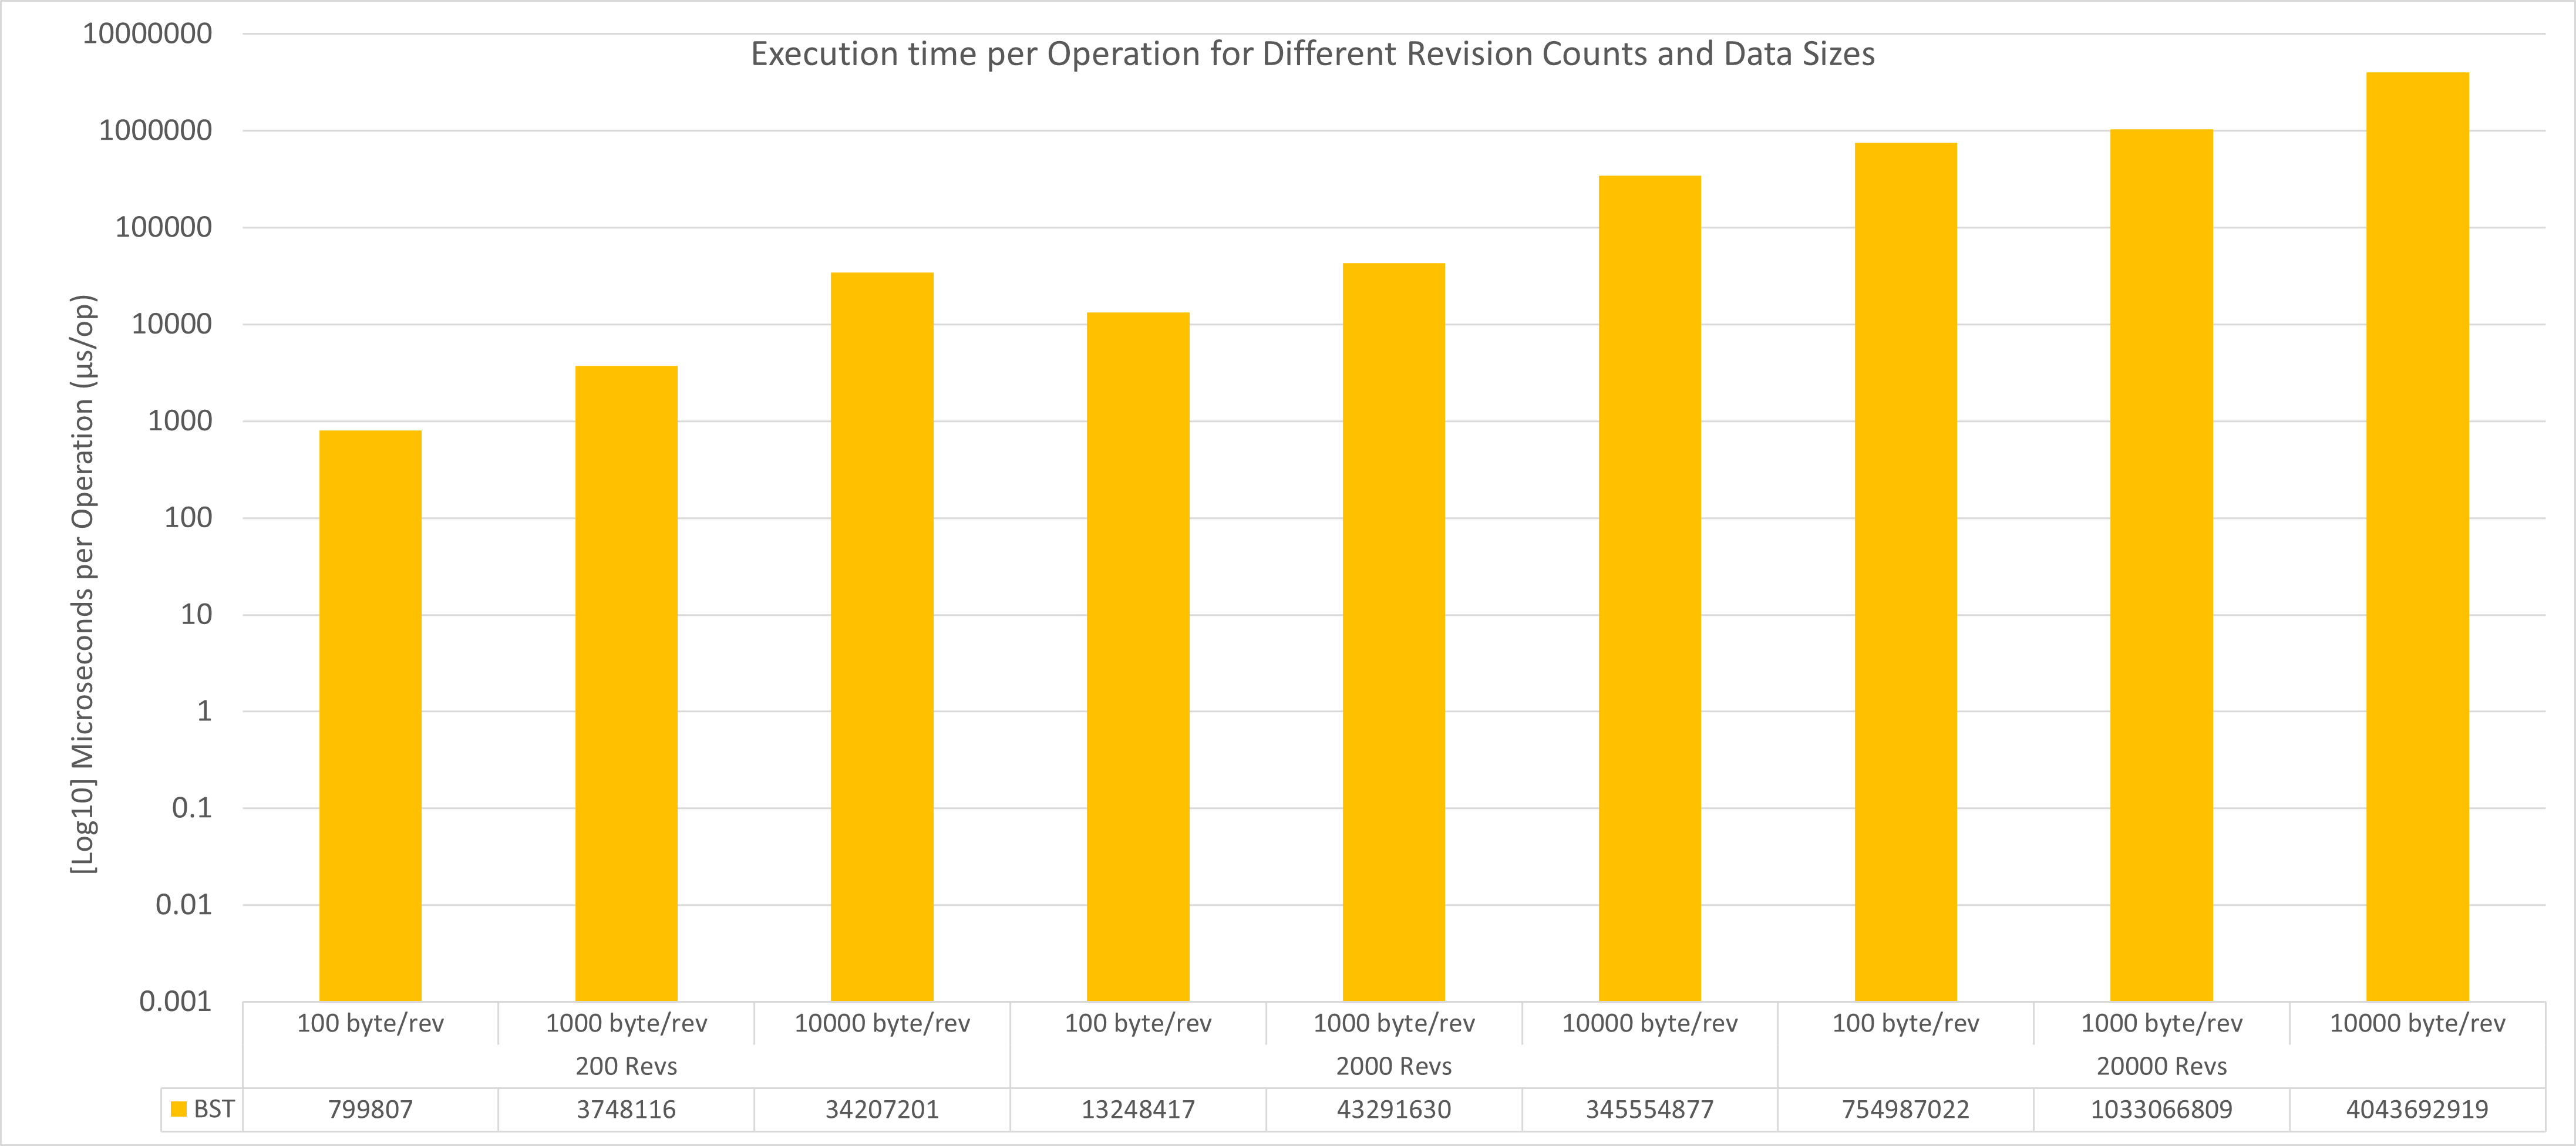
\includegraphics[width=1\linewidth]{charts/bst_ns_all.png}
        \caption{Execution Time}
        \label{fig:binary-search-tree-execution-time}
    \end{subfigure}

    \begin{subfigure}[b]{0.8\textwidth}
        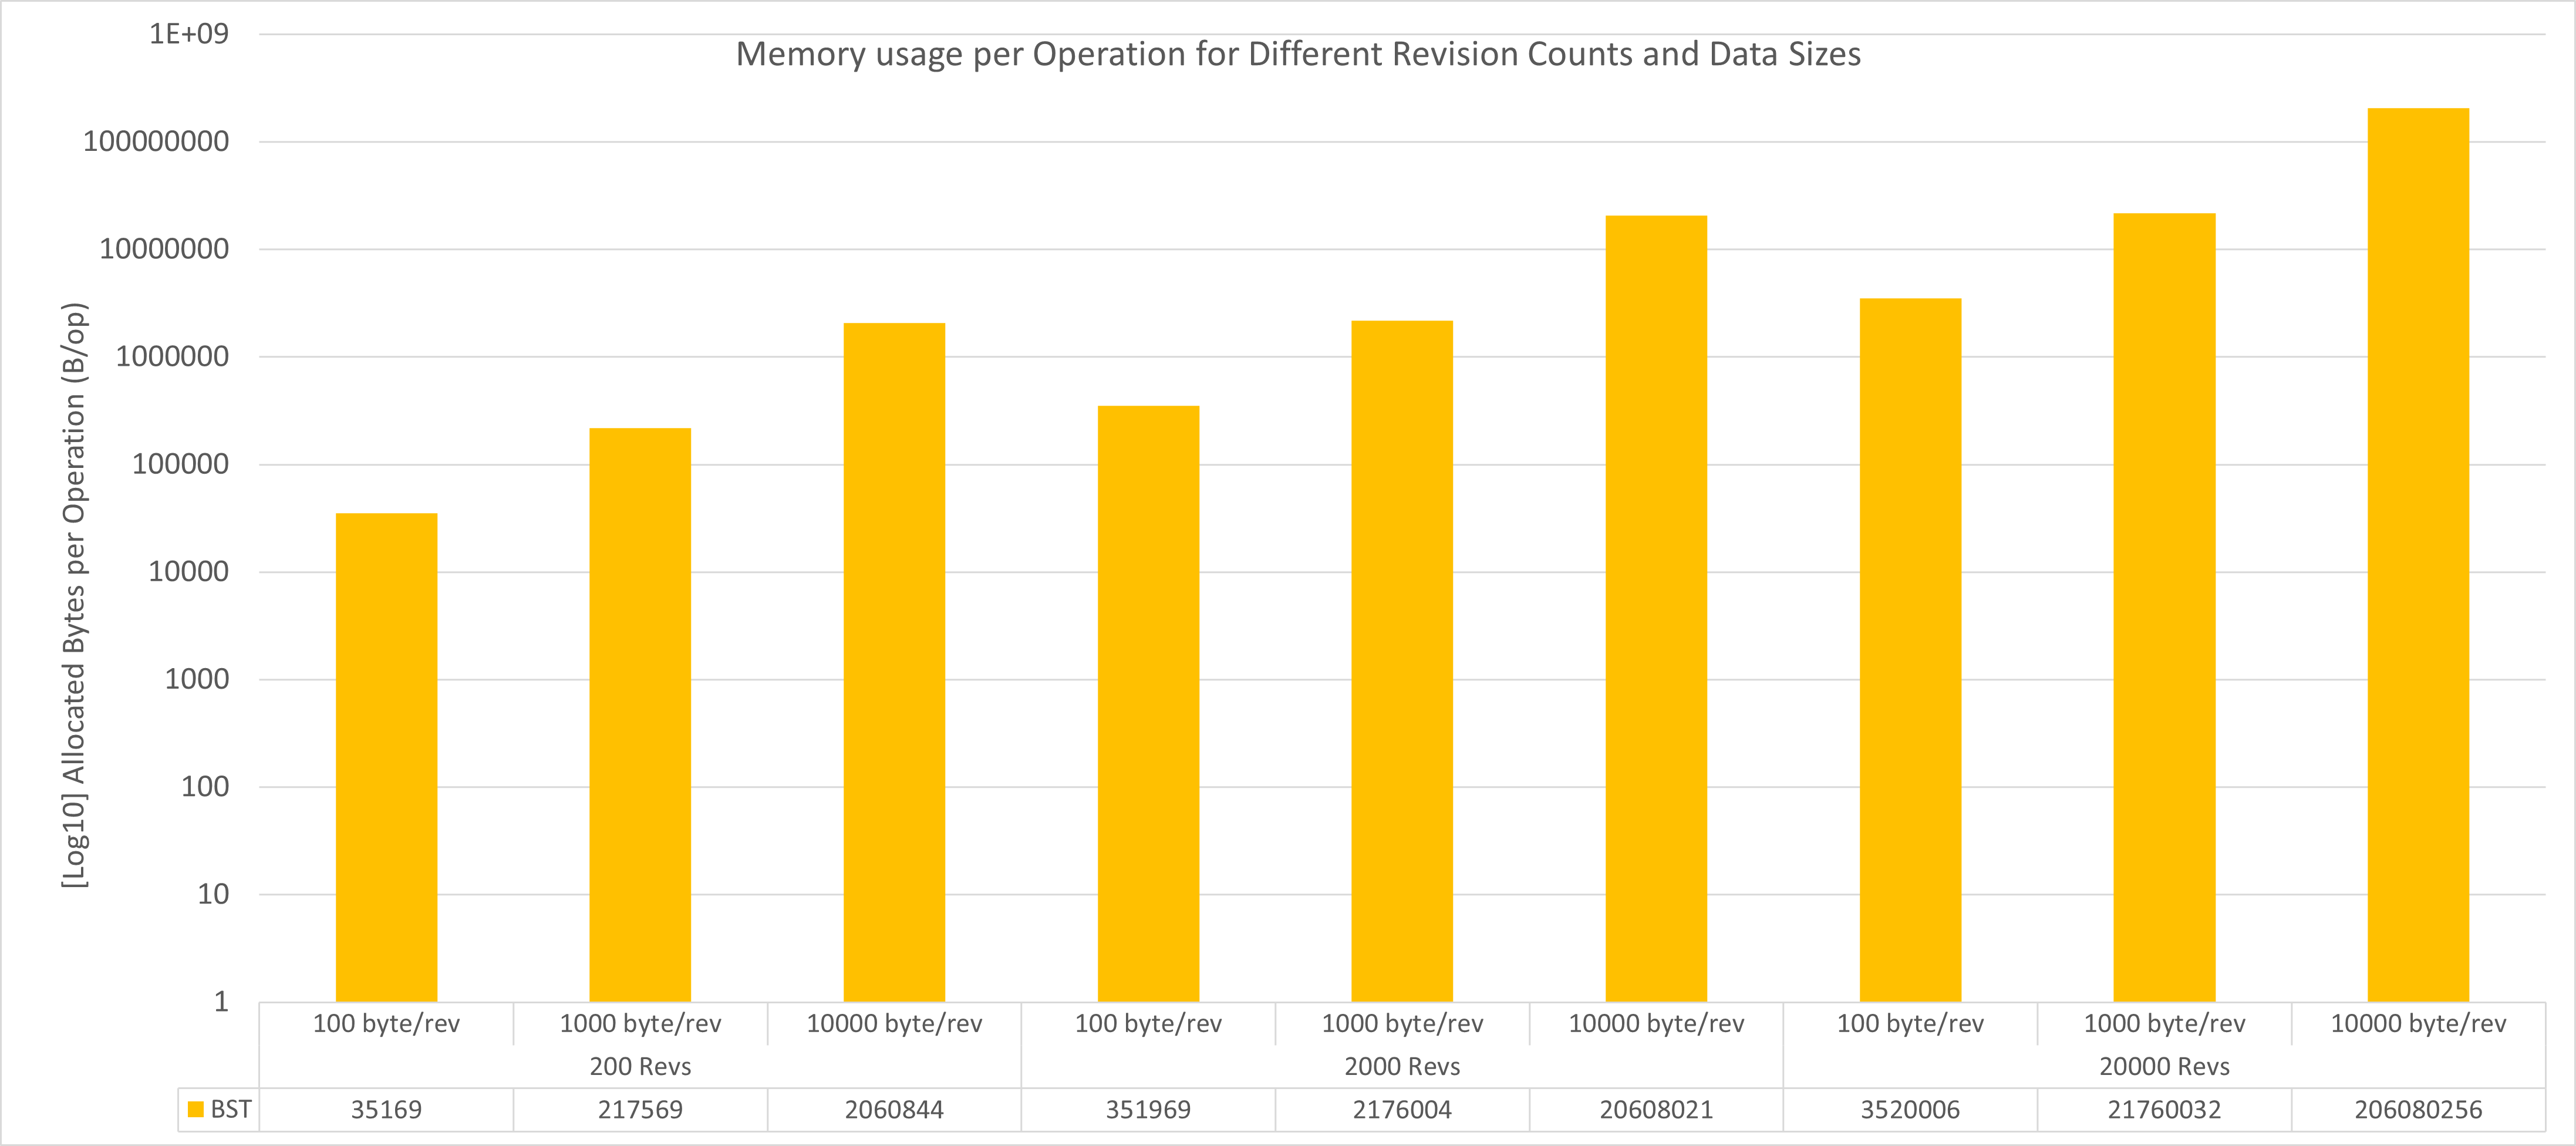
\includegraphics[width=1\linewidth]{charts/bst_bytes_all.png}
        \caption{Memory Usage}
        \label{fig:binary-search-tree-memory-usage}
    \end{subfigure}

    \begin{subfigure}[b]{0.8\textwidth}
        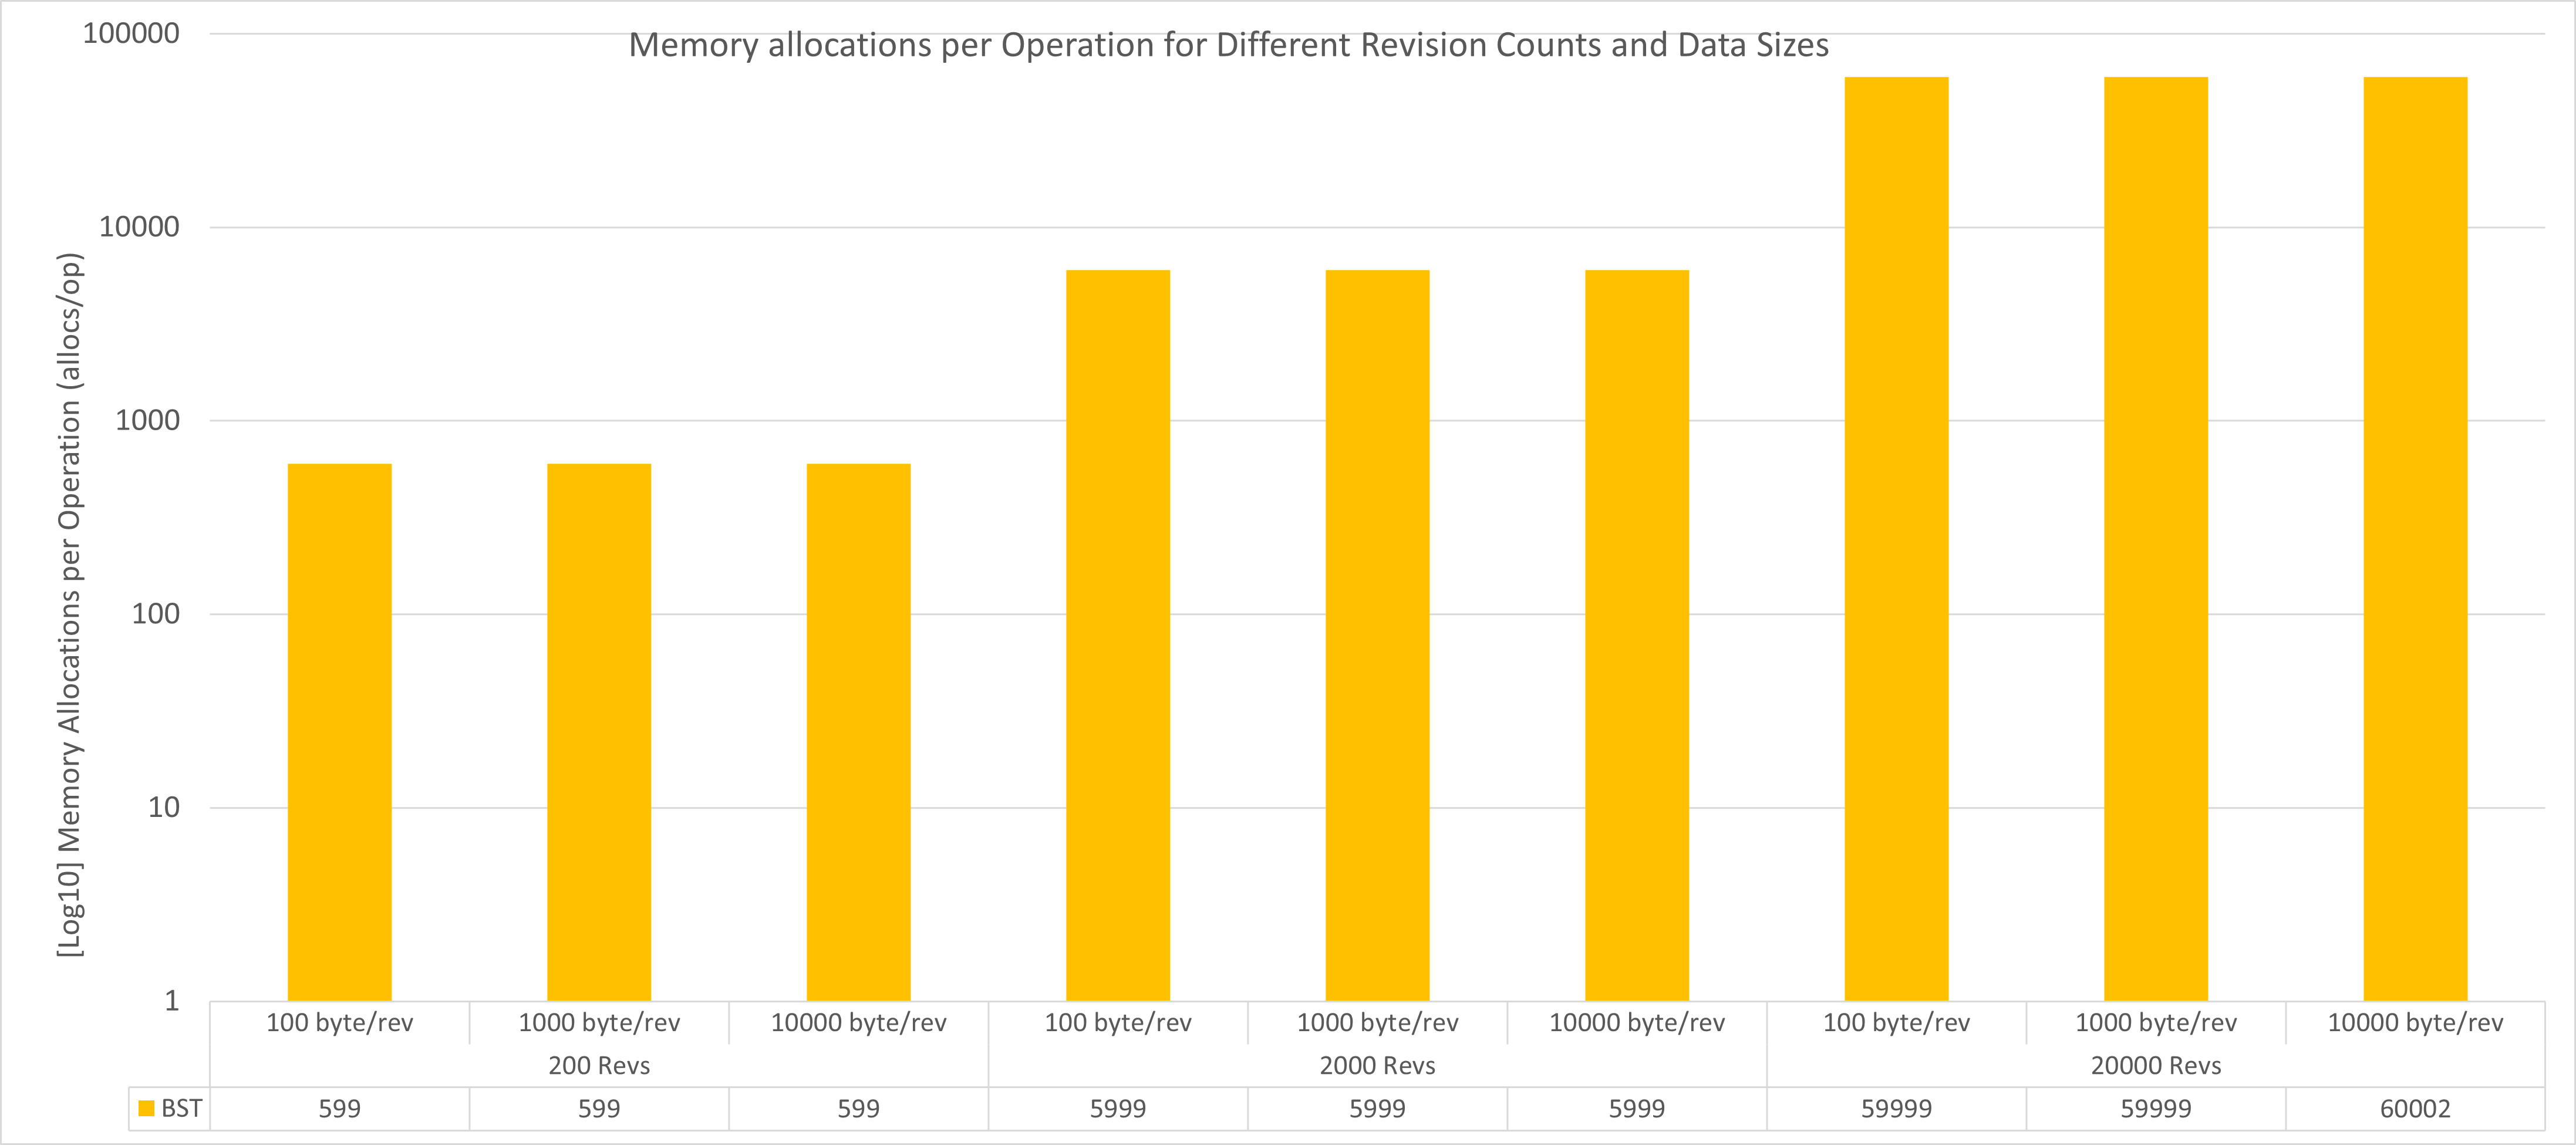
\includegraphics[width=1\linewidth]{charts/bst_allocs_all.png}
        \caption{Memory Allocations}
        \label{fig:binary-search-tree-memory-allocations}
    \end{subfigure}

    \caption{Performance metrics for the Binary Search Tree implementation.}
    \label{fig:binary-search-tree-performance-metrics}
\end{figure}

\subsection{Directed Acyclic Graph}

\begin{table}[h]
    \centering
    \begin{tabular}{|r|r|r|r|r|}
        \hline
        \multicolumn{1}{|c|}{\textbf{num\_revisions}} & \multicolumn{1}{c|}{\textbf{data\_size}} & \multicolumn{1}{c|}{\textbf{ns\_per\_op}} & \multicolumn{1}{c|}{\textbf{bytes\_per\_op}} & \multicolumn{1}{c|}{\textbf{allocs\_per\_op}} \\ \hline
        200 Revs                                      & 100 byte/rev                             & 727843                                    & 55593                                        & 1008                                          \\ \hline
        200 Revs                                      & 1000 byte/rev                            & 3734667                                   & 237970                                       & 1008                                          \\ \hline
        200 Revs                                      & 10000 byte/rev                           & 34303289                                  & 2081246                                      & 1009                                          \\ \hline
        2000 Revs                                     & 100 byte/rev                             & 7260065                                   & 618806                                       & 10057                                         \\ \hline
        2000 Revs                                     & 1000 byte/rev                            & 37559841                                  & 2442897                                      & 10058                                         \\ \hline
        2000 Revs                                     & 10000 byte/rev                           & 343197450                                 & 20875066                                     & 10057                                         \\ \hline
        20000 Revs                                    & 100 byte/rev                             & 73485424                                  & 5824547                                      & 100473                                        \\ \hline
        20000 Revs                                    & 1000 byte/rev                            & 374157517                                 & 24065936                                     & 100484                                        \\ \hline
        20000 Revs                                    & 10000 byte/rev                           & 3492010230                                & 208384192                                    & 100473                                        \\ \hline
    \end{tabular}
    \caption{Performance metrics for the Directed Acyclic Graph implementation.}
    \label{tab:directed-acyclic-graph-benchmark-results}
\end{table}

\begin{figure}[H]
    \centering
    \begin{subfigure}[b]{0.8\textwidth}
        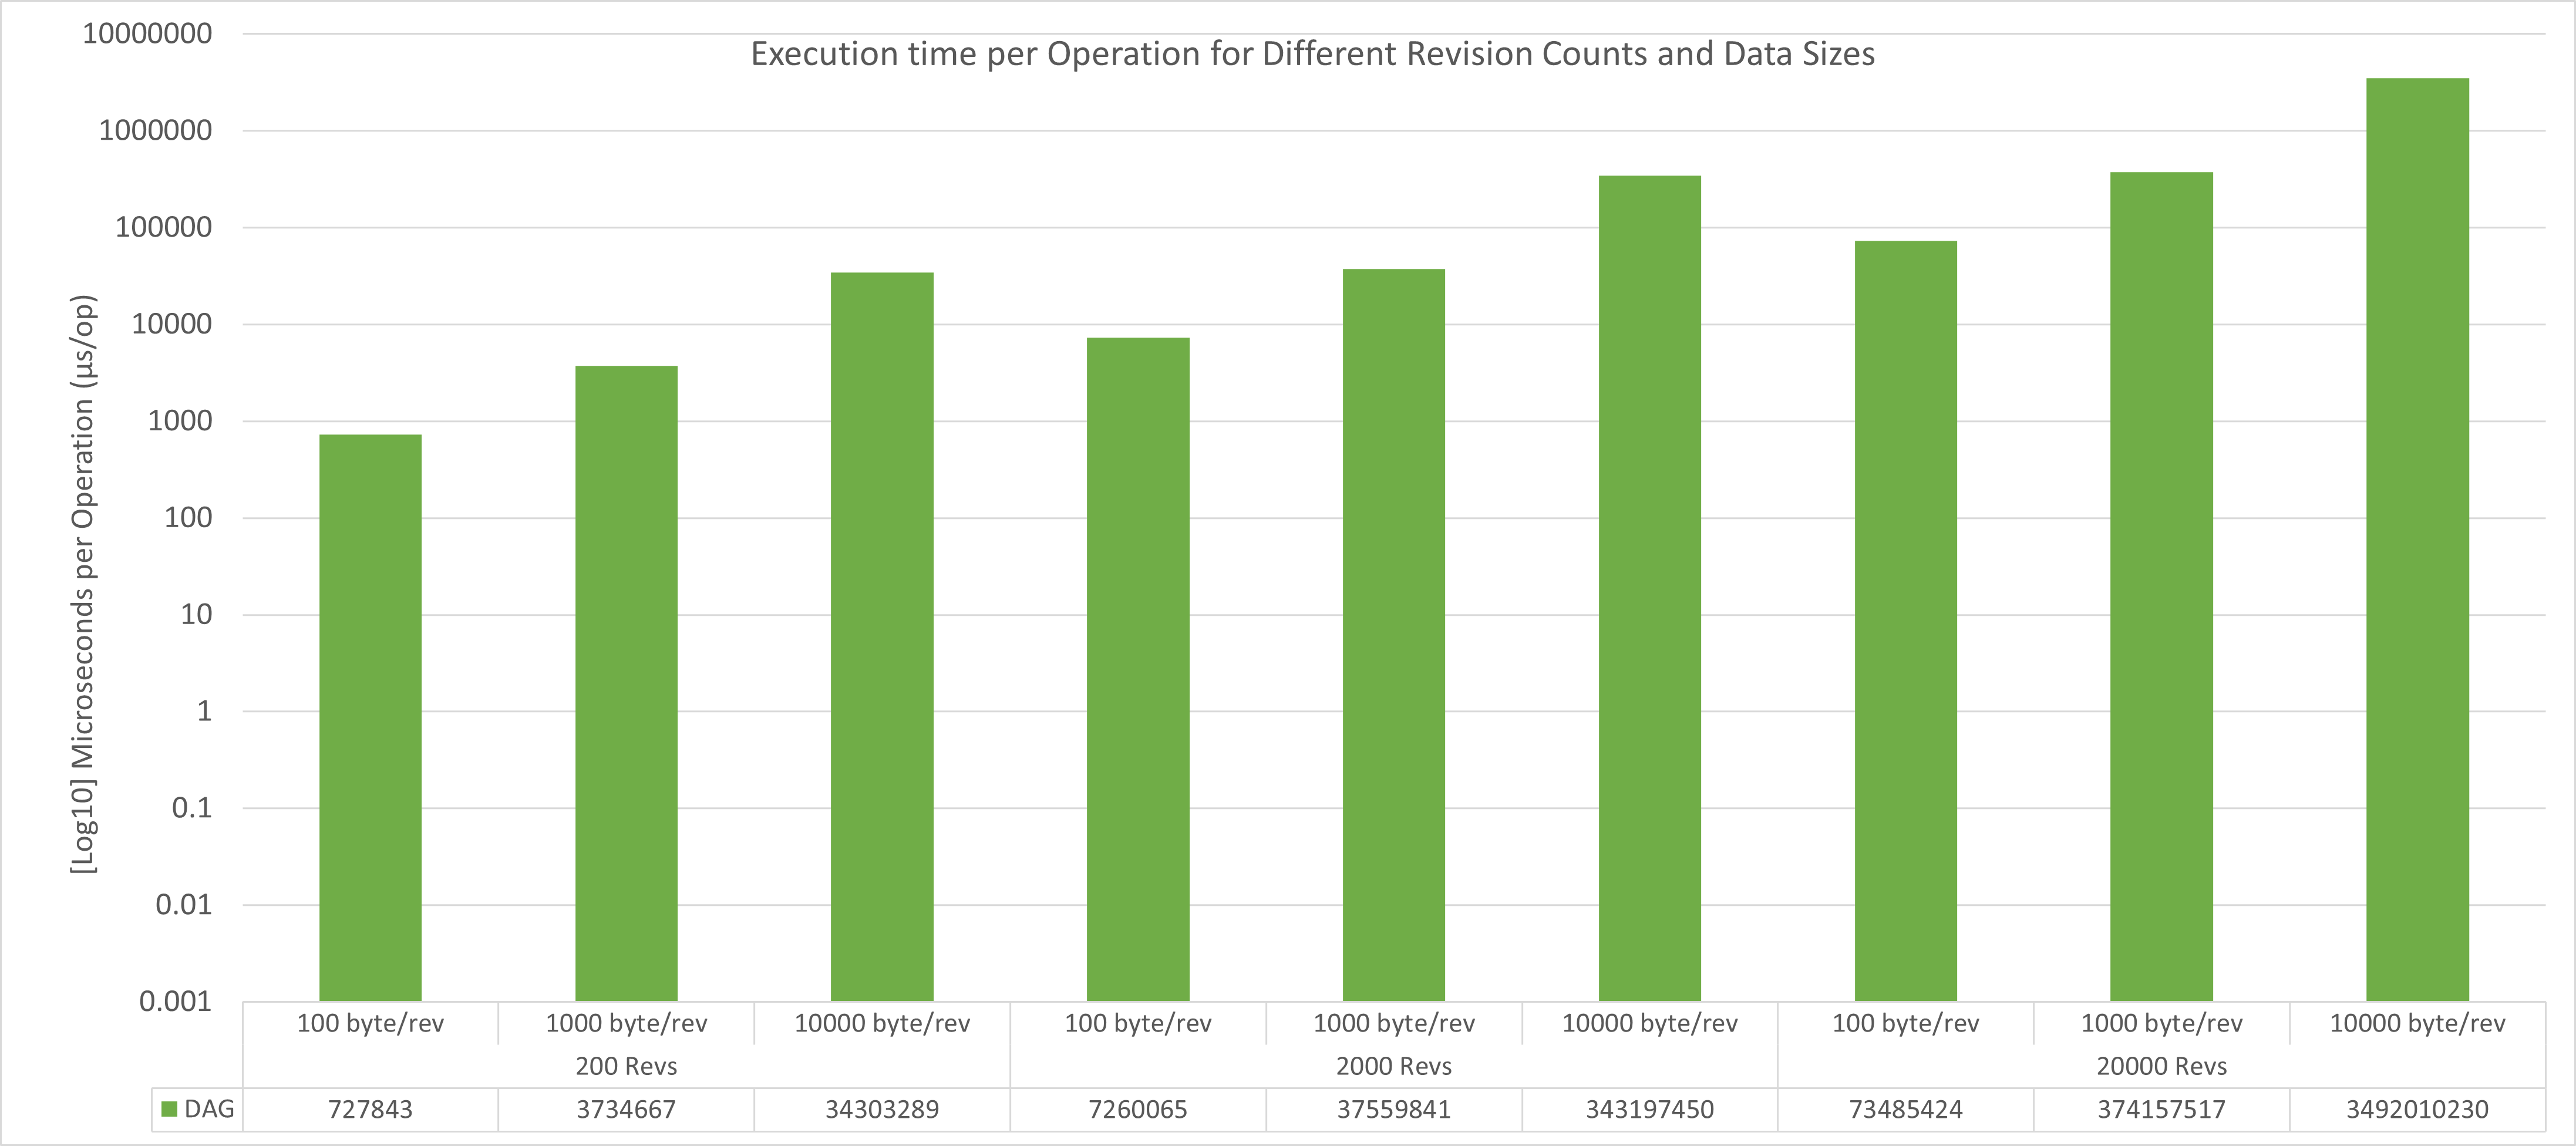
\includegraphics[width=1\linewidth]{charts/dag_ns_all.png}
        \caption{Execution Time}
        \label{fig:directed-acyclic-graph-execution-time}
    \end{subfigure}

    \begin{subfigure}[b]{0.8\textwidth}
        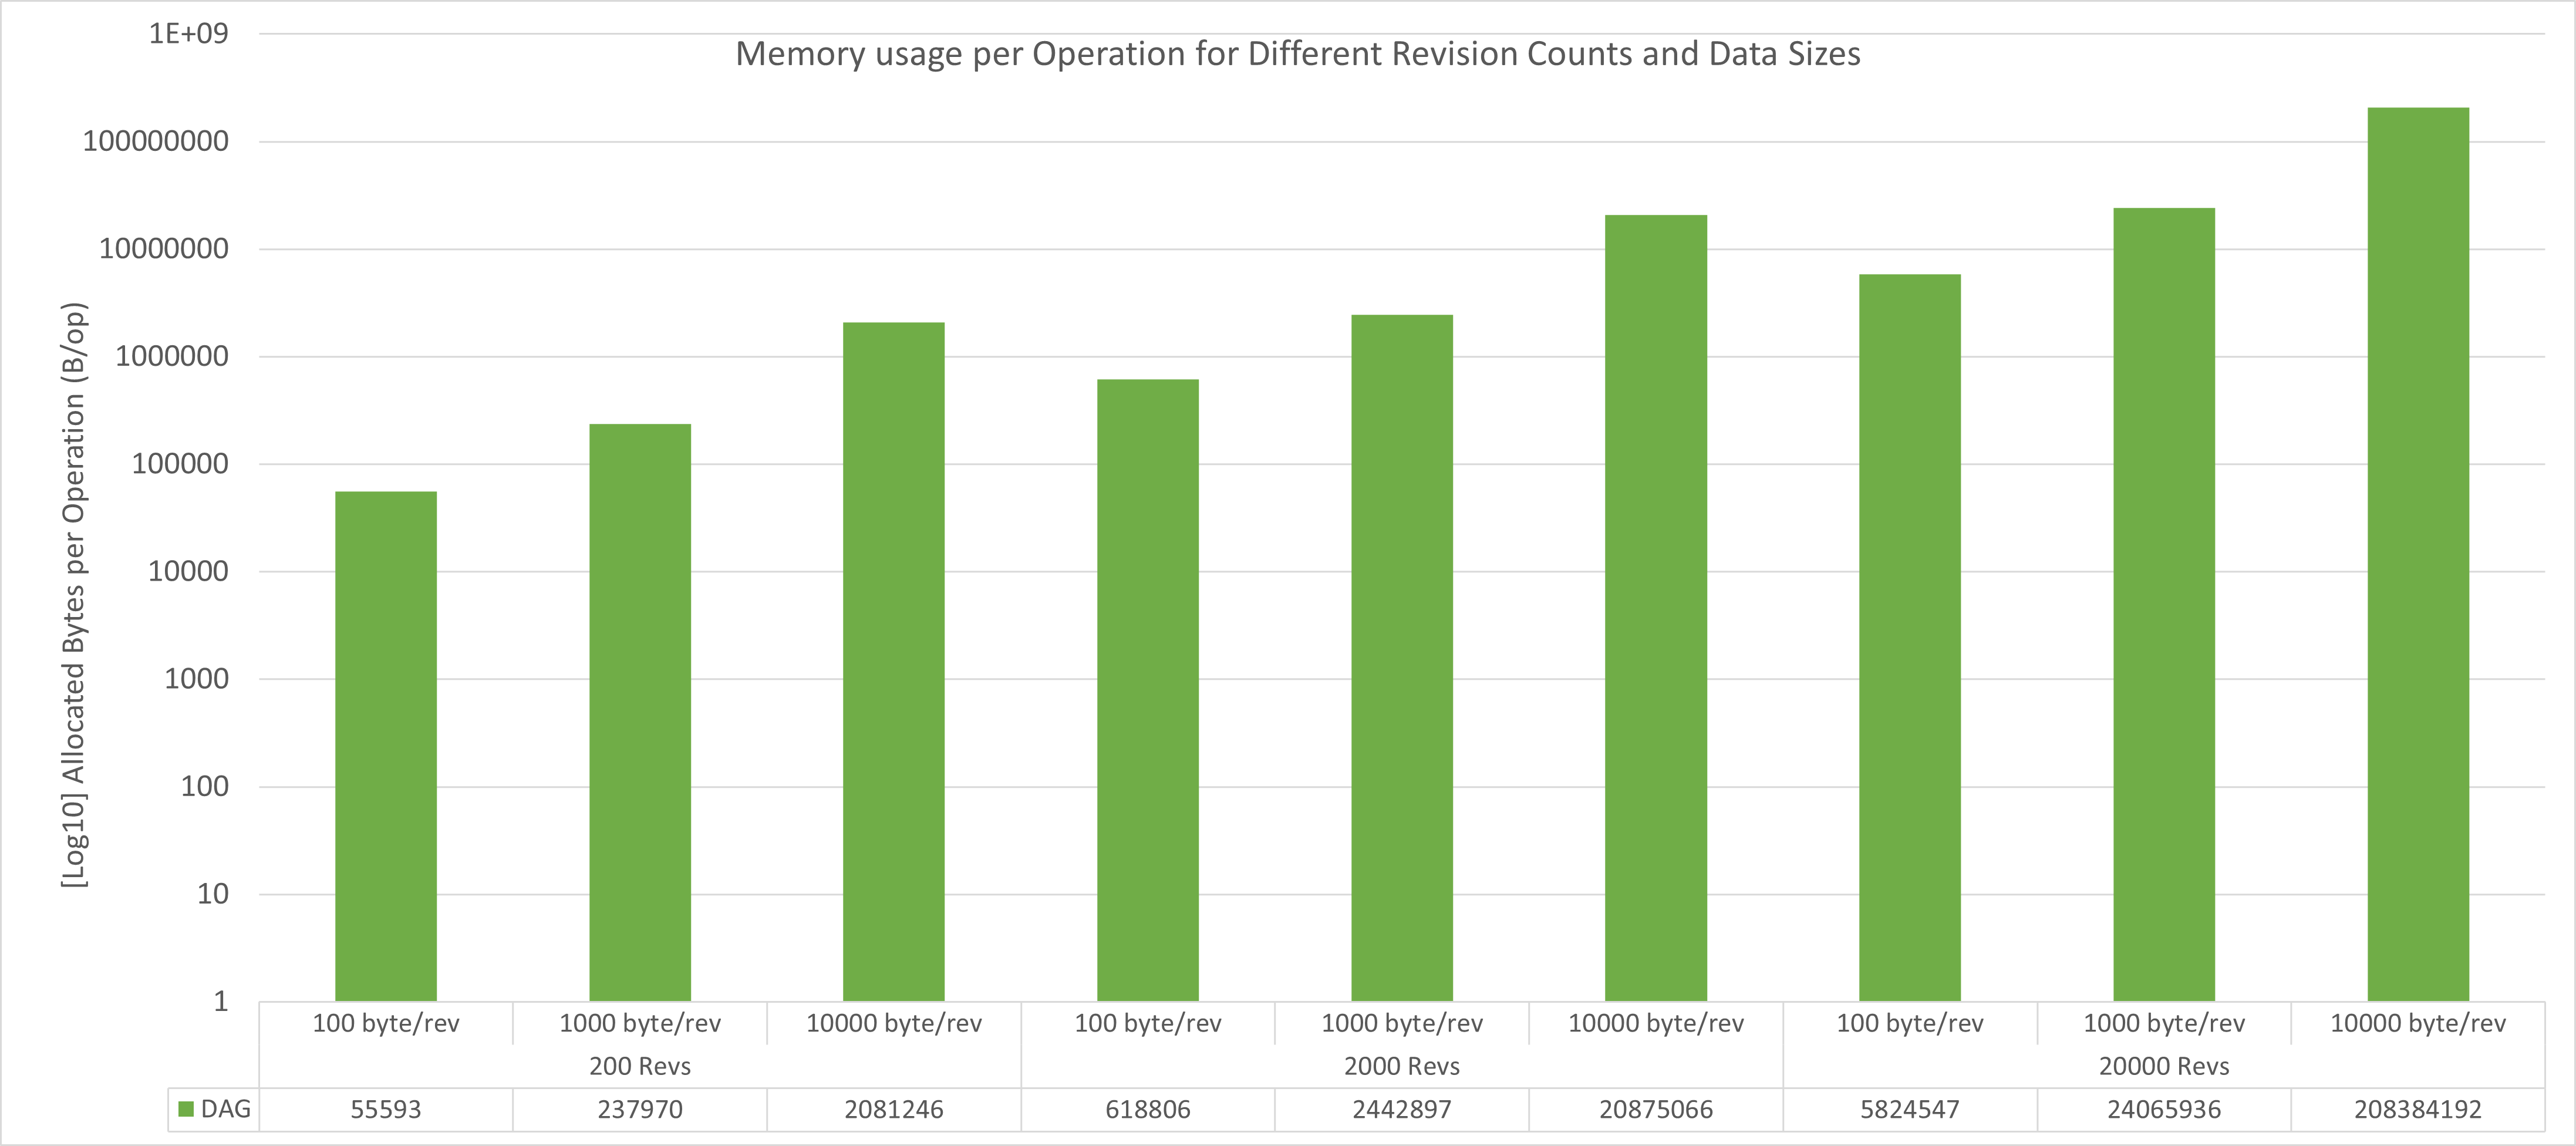
\includegraphics[width=1\linewidth]{charts/dag_bytes_all.png}
        \caption{Memory Usage}
        \label{fig:directed-acyclic-graph-memory-usage}
    \end{subfigure}

    \begin{subfigure}[b]{0.8\textwidth}
        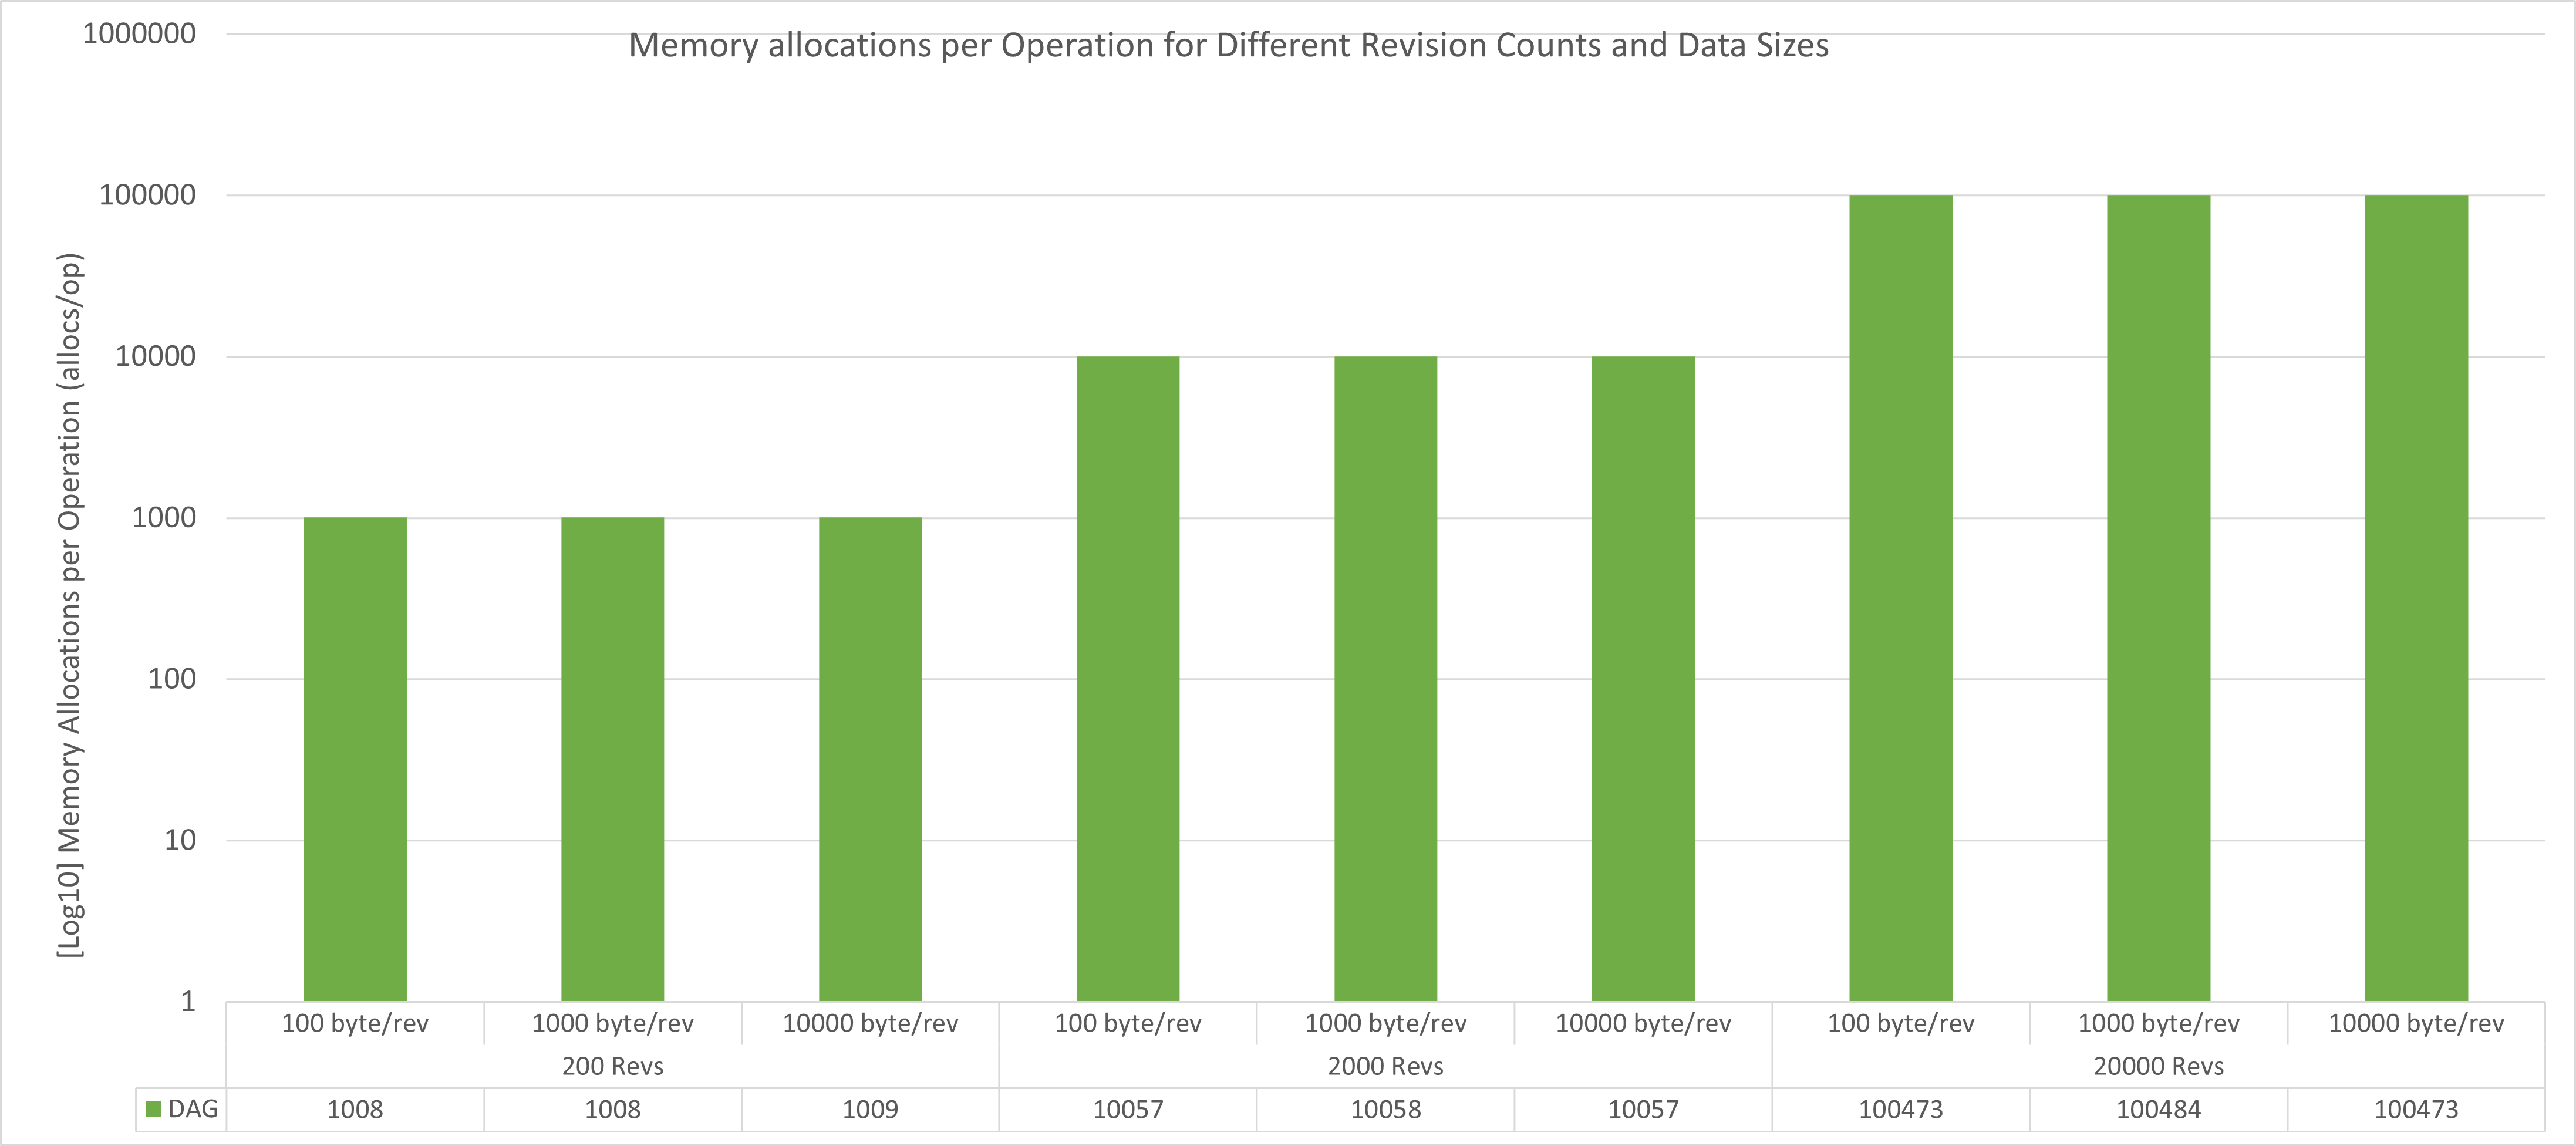
\includegraphics[width=1\linewidth]{charts/dag_allocs_all.png}
        \caption{Memory Allocations}
        \label{fig:directed-acyclic-graph-memory-allocations}
    \end{subfigure}

    \caption{Performance metrics for the Directed Acyclic Graph implementation.}
    \label{fig:directed-acyclic-graph-performance-metrics}
\end{figure}

\subsection{Comparison}

\begin{figure}[H]
    \centering
    \begin{subfigure}[b]{0.75\textwidth}
        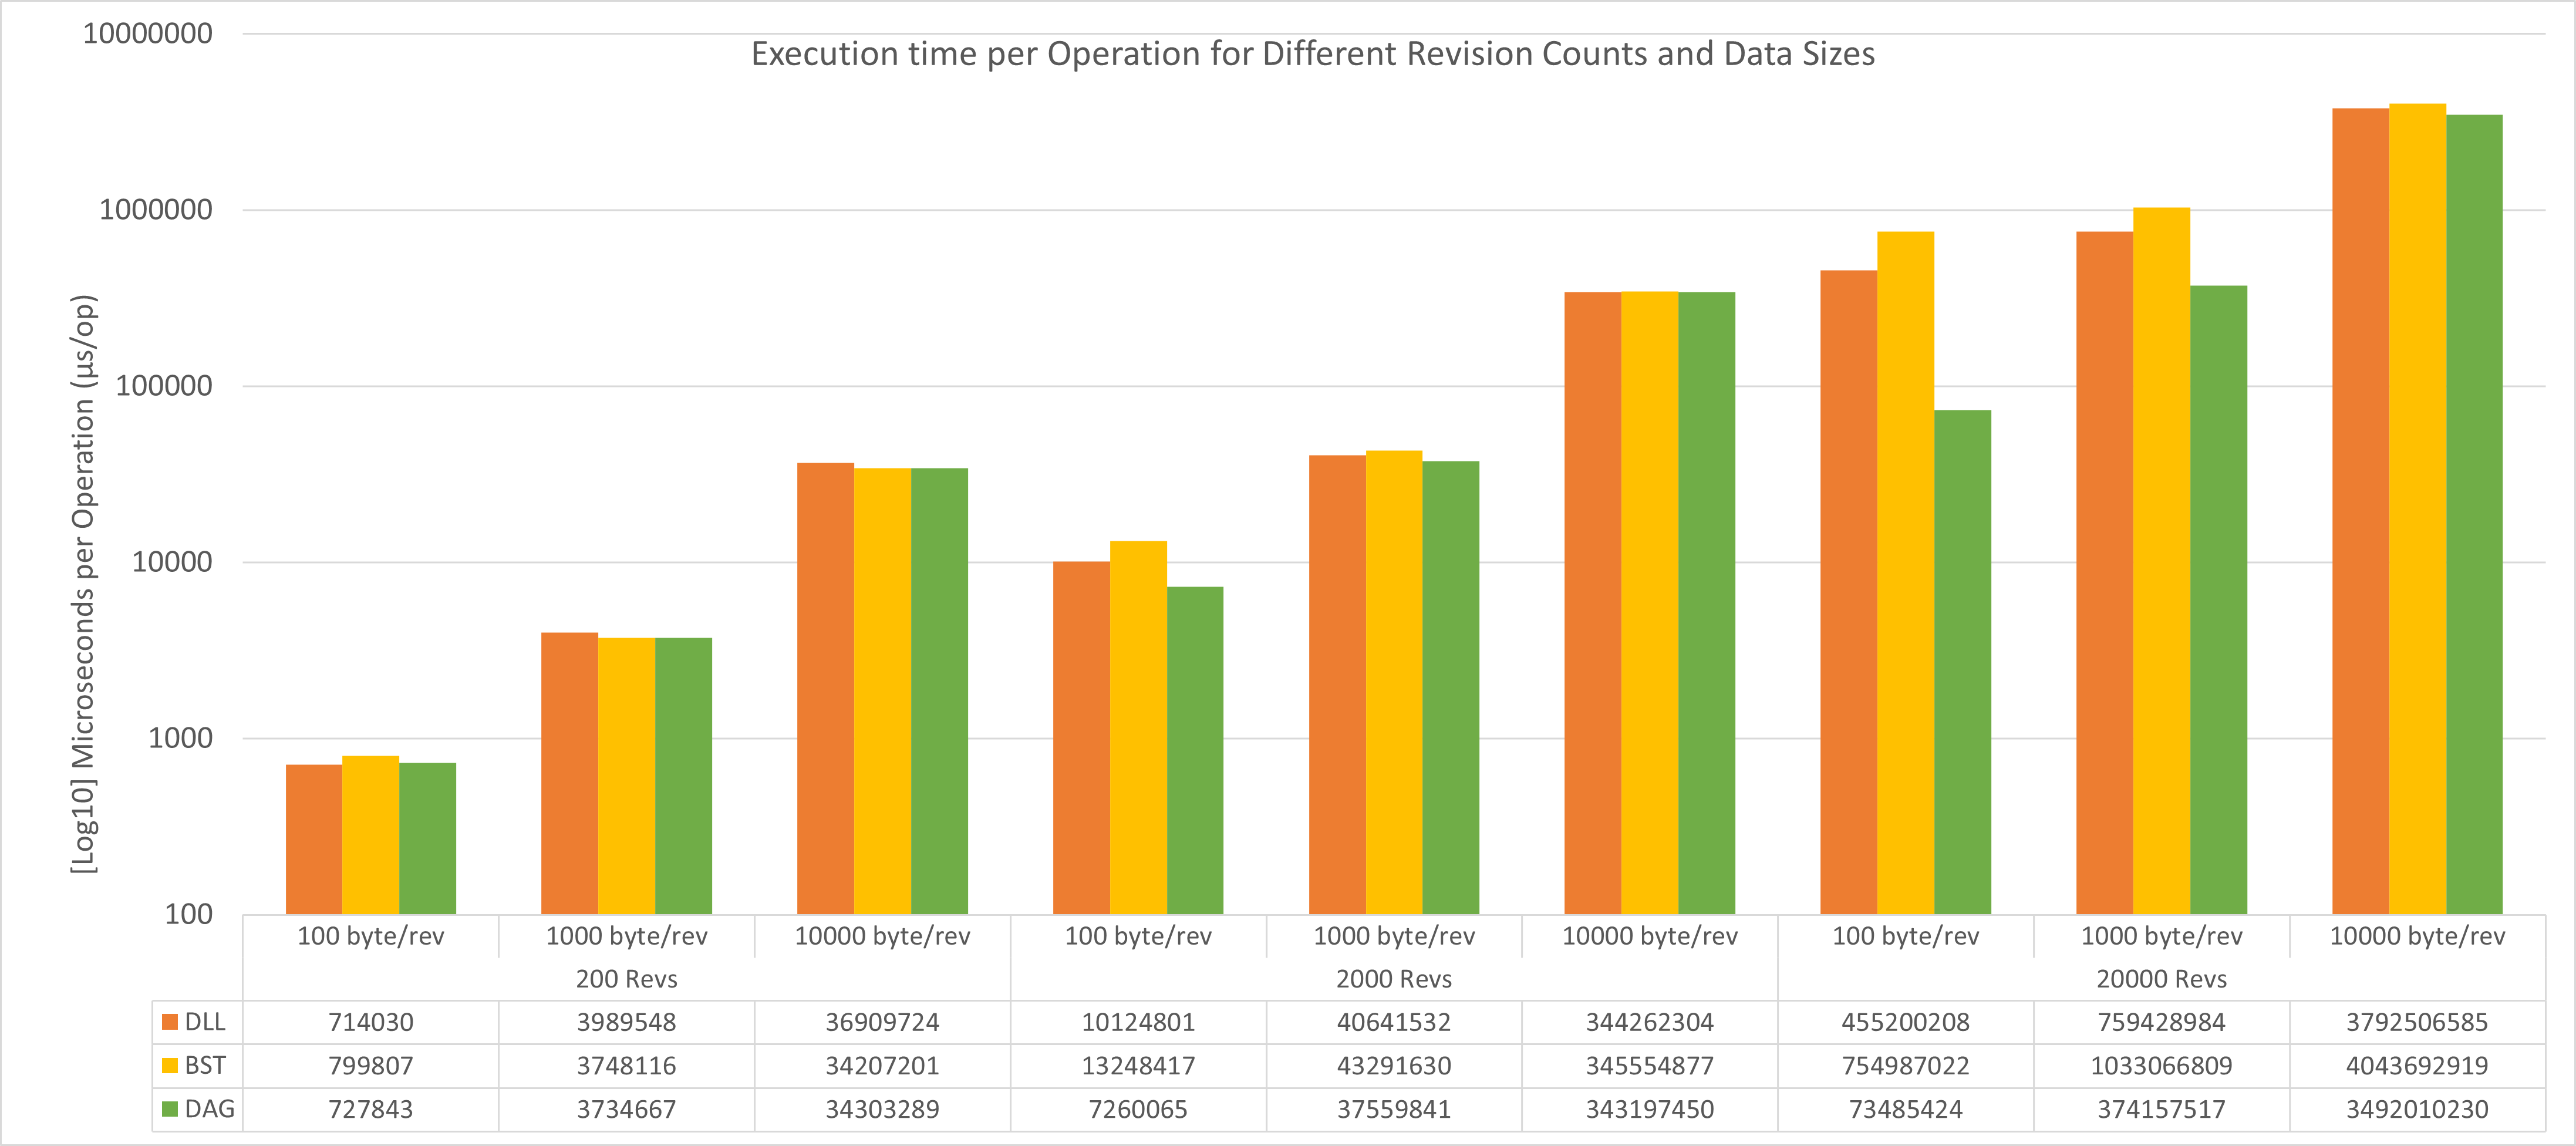
\includegraphics[width=1\linewidth]{charts/dataStruct_ns_all.png}
        \caption{Execution Time}
        \label{fig:data-structure-execution-time}
    \end{subfigure}

    \begin{subfigure}[b]{0.75\textwidth}
        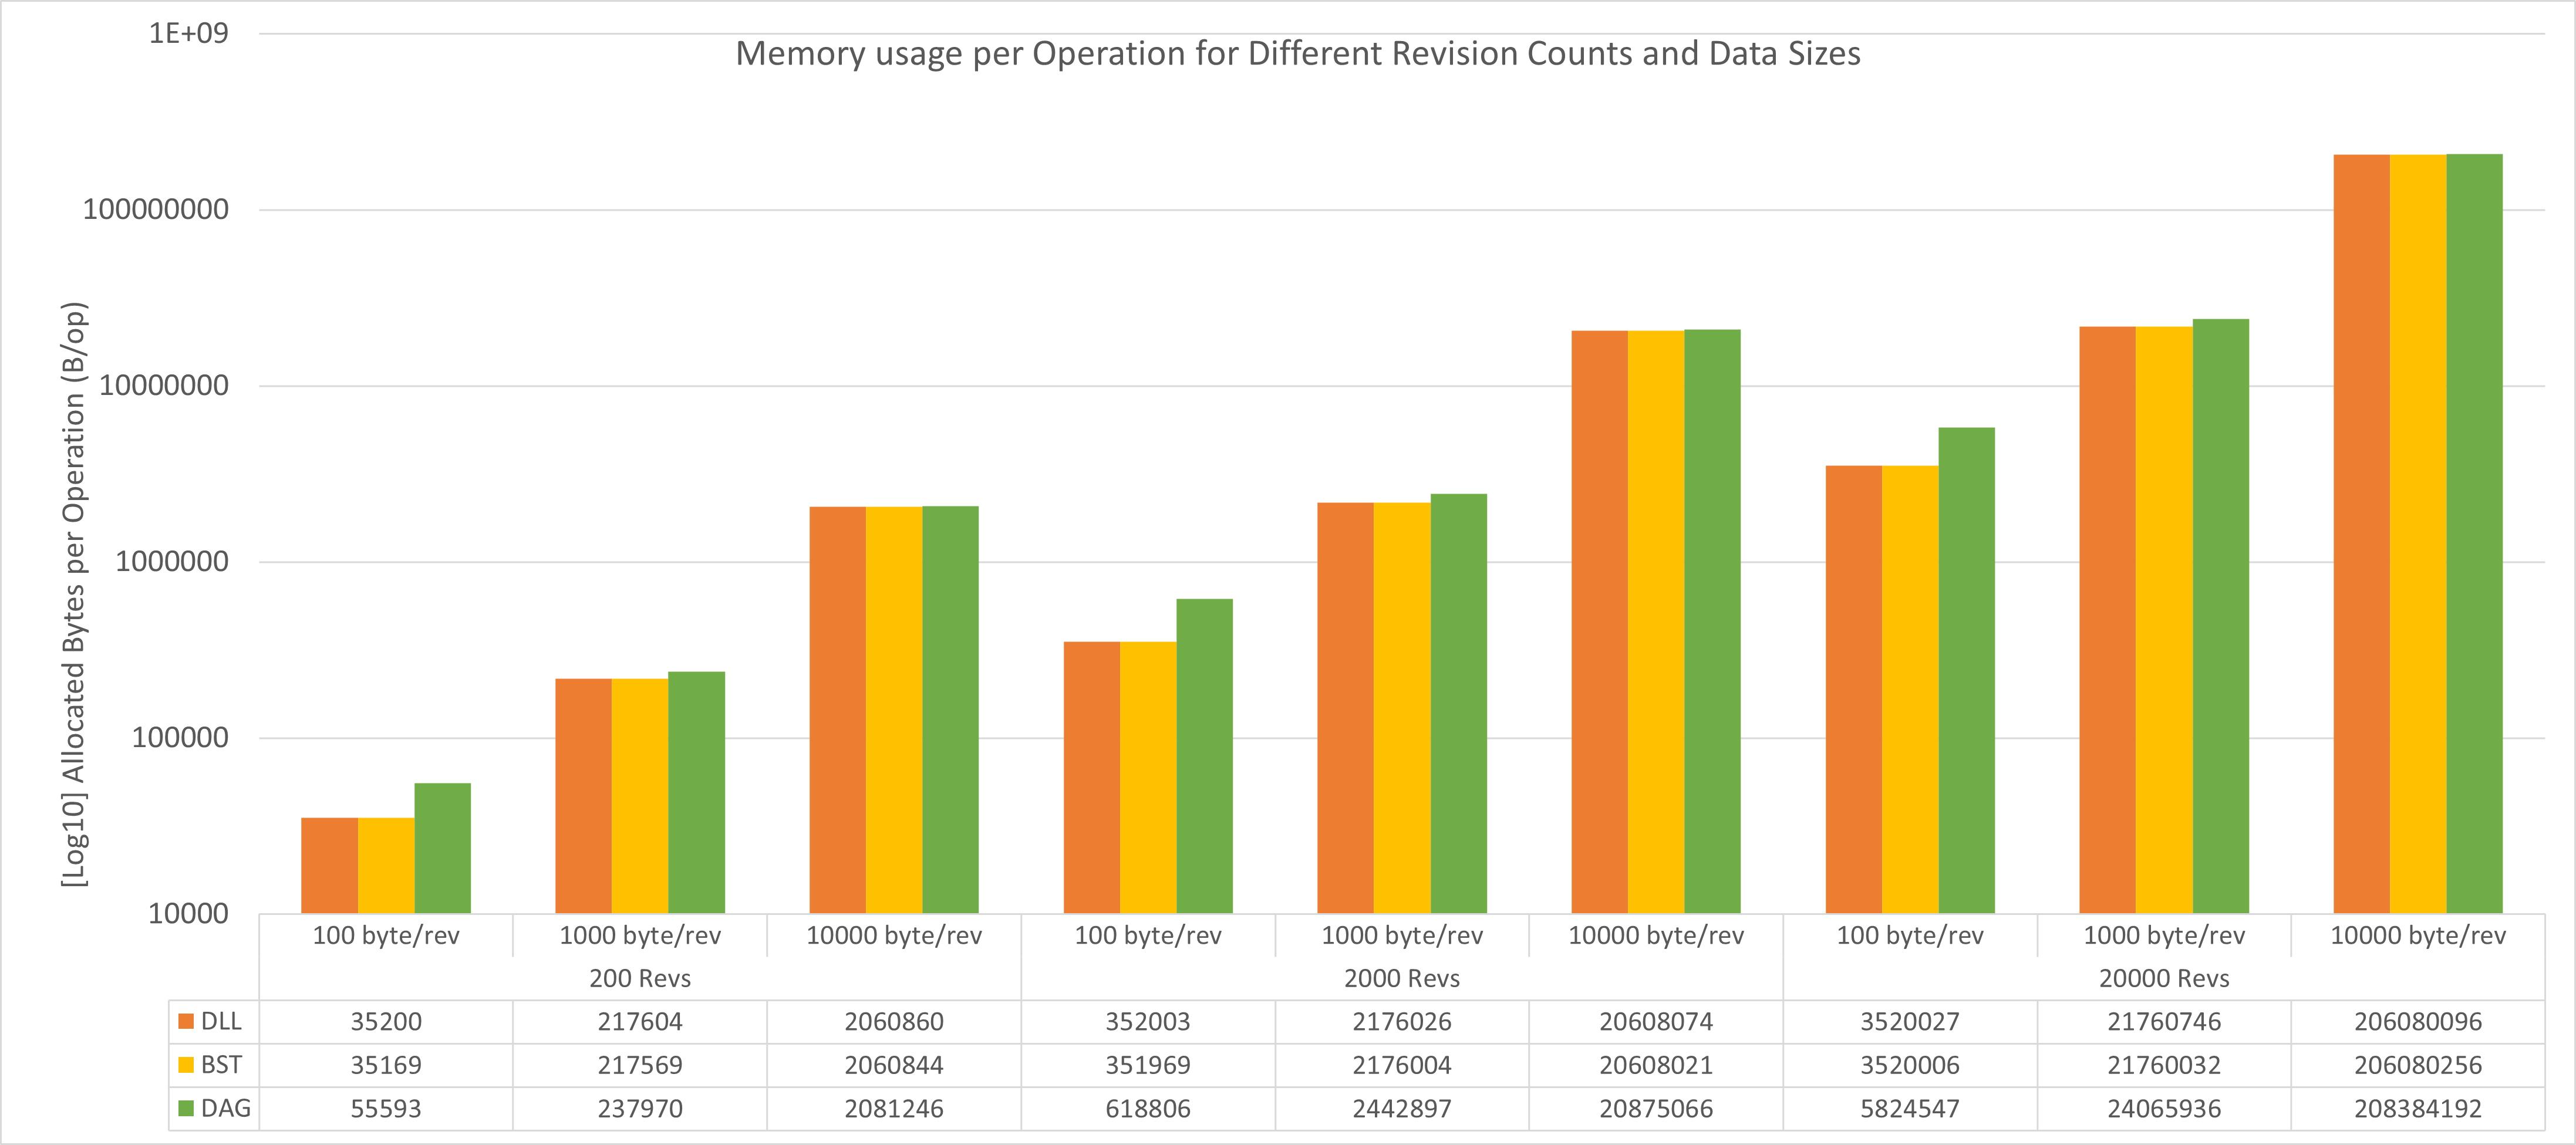
\includegraphics[width=1\linewidth]{charts/dataStruct_bytes_all.png}
        \caption{Memory Usage}
        \label{fig:data-structure-memory-usage}
    \end{subfigure}

    \begin{subfigure}[b]{0.75\textwidth}
        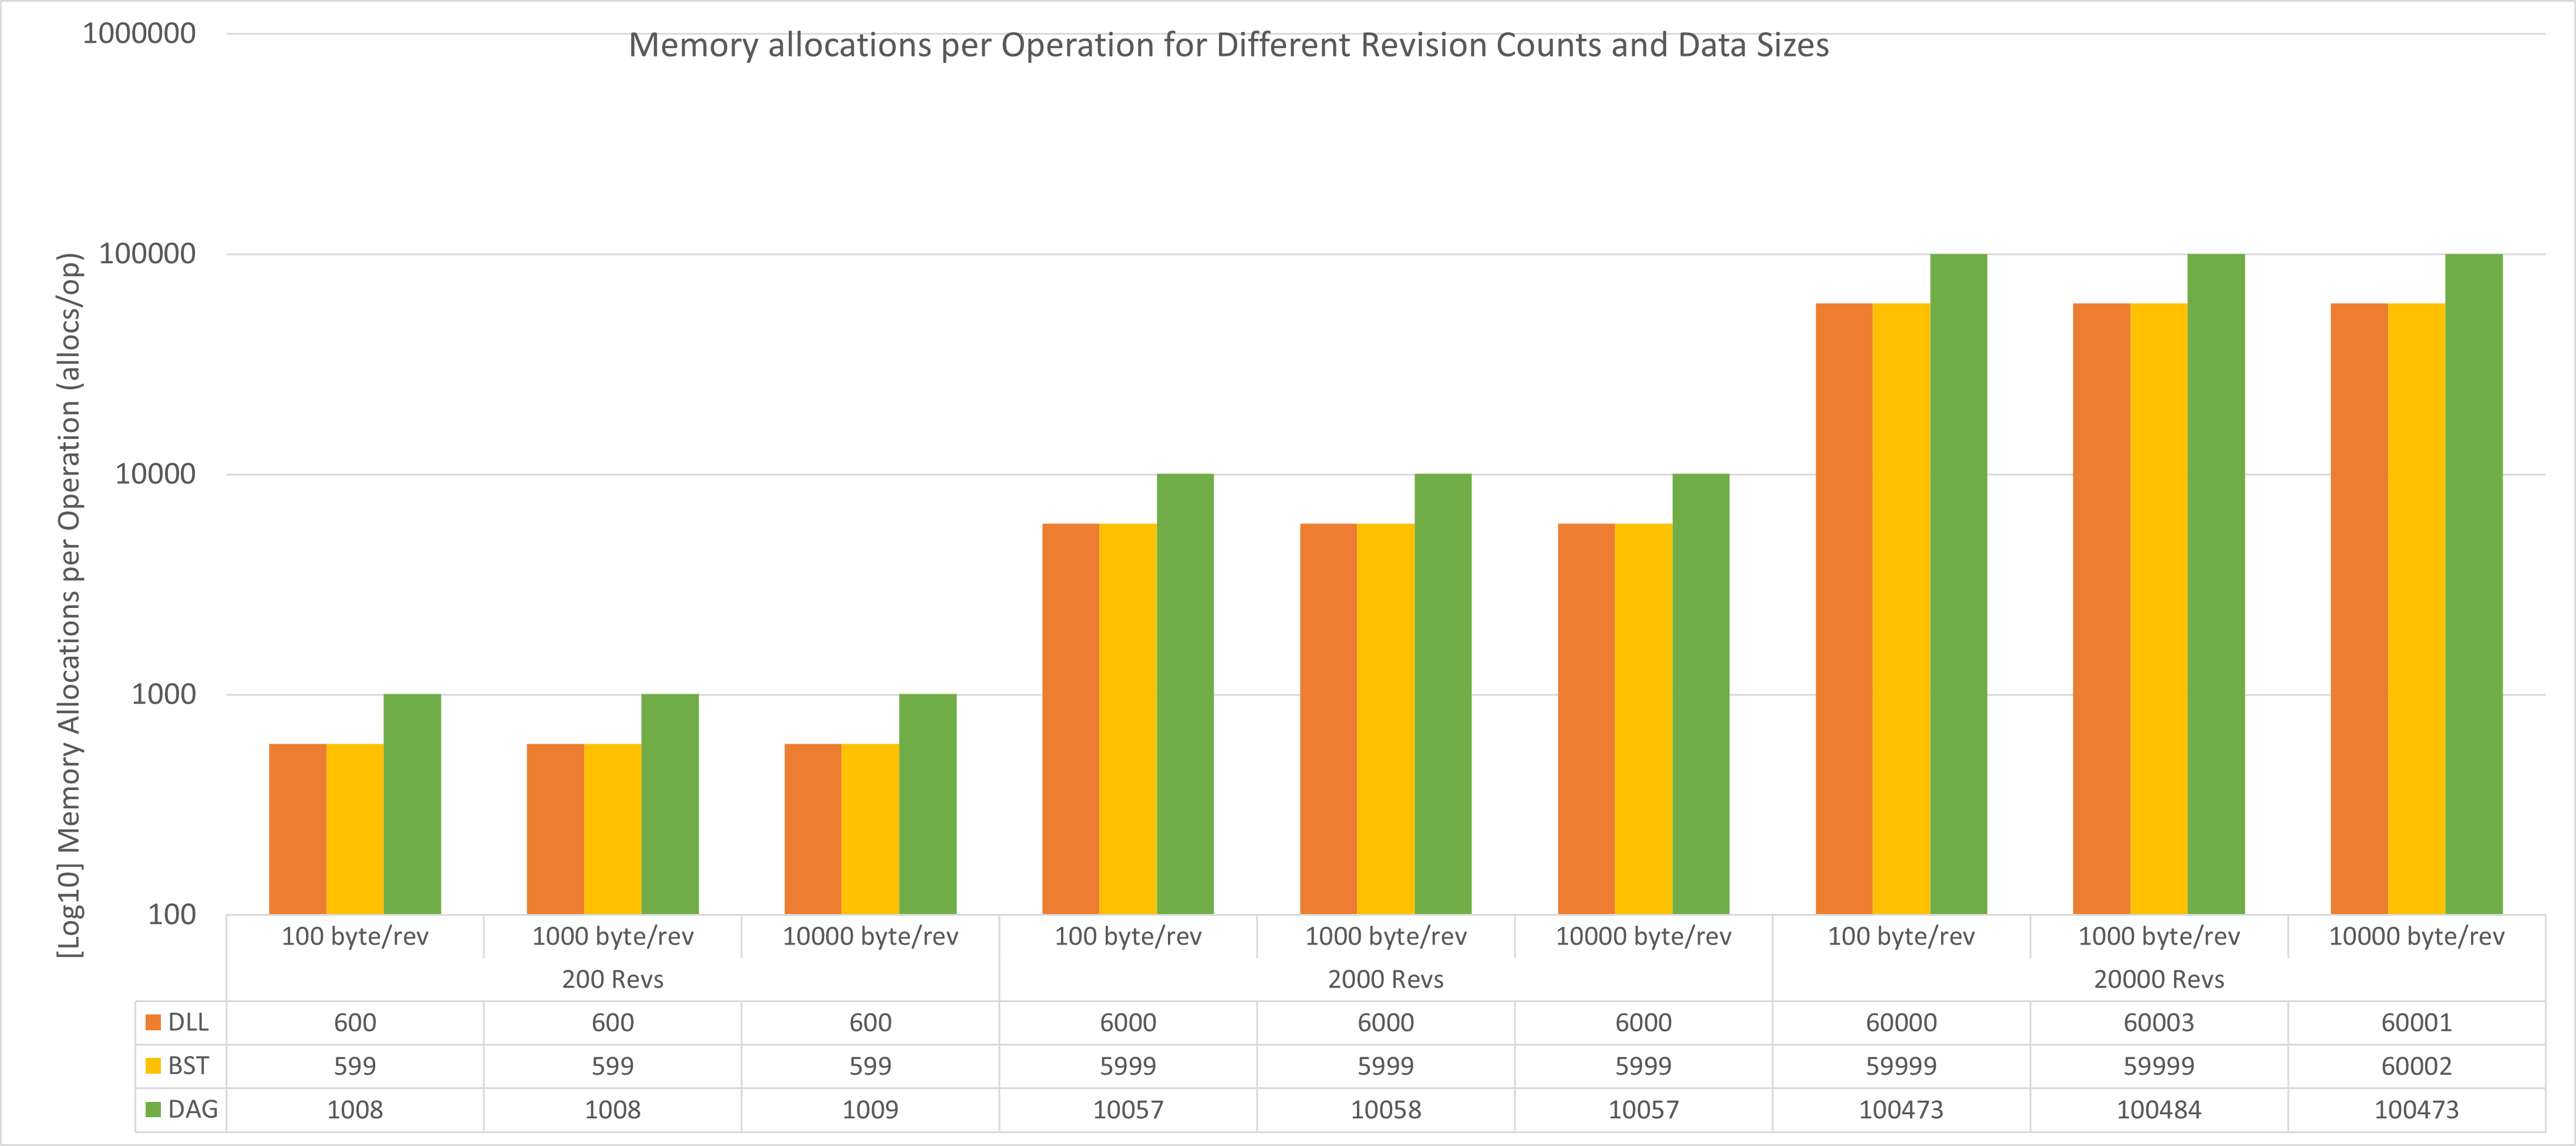
\includegraphics[width=1\linewidth]{charts/dataStruct_allocs_all.png}
        \caption{Memory Allocations}
        \label{fig:data-structure-memory-allocations}
    \end{subfigure}

    \caption{Performance metrics for all three Data Structure implementations.}
    \label{fig:data-structure-performance-metrics}
\end{figure}
\newpage

\paragraph{Execution Time}
Regarding execution time across the three data structures, we see that \lstinline{numRevisions} seems to have the most significant impact on the processing time, especially when the number of revisions is high. For a low and medium number of revisions, all three data structures have similar performance. However, once the number of revisions grows large enough, we start to see the \lstinline{Directed Acyclic Graph} handling small data sizes much better than the \lstinline{Doubly Linked List} and \lstinline{Binary Search Tree}.
\smallskip

\paragraph{Memory Usage}
The memory usage for the \lstinline{Doubly Linked List} and \lstinline{Binary Search Tree} appears to be relatively equal across all data sizes. However, the \lstinline{Directed Acyclic Graph} seems to require more memory at low and medium data sizes. This is likely due to the fact that the \lstinline{Directed Acyclic Graph} is storing the data in a map, which is a hash table. The \lstinline{Doubly Linked List} and \lstinline{Binary Search Tree} are storing the data in a slice, which is a contiguous block of memory.
\smallskip

\paragraph{Memory Allocations}
The memory allocation data mirrors the memory usage data, showing similar performance across the board for the \lstinline{Doubly Linked List} and \lstinline{Binary Search Tree} but higher memory requirements for the \lstinline{Directed Acyclic Graph}.

\section{Algorithms}

\subsection{Search Algorithms}

\begin{table}[h]
    \centering
    \begin{tabular}{|r|r|r|r|r|}
        \hline
        \multicolumn{1}{|c|}{\textbf{num\_revisions}} & \multicolumn{1}{c|}{\textbf{data\_size}} & \multicolumn{1}{c|}{\textbf{ns\_per\_op}} & \multicolumn{1}{c|}{\textbf{bytes\_per\_op}} & \multicolumn{1}{c|}{\textbf{allocs\_per\_op}} \\ \hline
        200 Revs                                      & 100 byte/rev                             & 192                                       & 0                                            & 0                                             \\ \hline
        200 Revs                                      & 1000 byte/rev                            & 191                                       & 0                                            & 0                                             \\ \hline
        200 Revs                                      & 10000 byte/rev                           & 190                                       & 0                                            & 0                                             \\ \hline
        2000 Revs                                     & 100 byte/rev                             & 1791                                      & 0                                            & 0                                             \\ \hline
        2000 Revs                                     & 1000 byte/rev                            & 1768                                      & 0                                            & 0                                             \\ \hline
        2000 Revs                                     & 10000 byte/rev                           & 1801                                      & 0                                            & 0                                             \\ \hline
        20000 Revs                                    & 100 byte/rev                             & 29180                                     & 0                                            & 0                                             \\ \hline
        20000 Revs                                    & 1000 byte/rev                            & 28773                                     & 0                                            & 0                                             \\ \hline
        20000 Revs                                    & 10000 byte/rev                           & 30309                                     & 0                                            & 0                                             \\ \hline
    \end{tabular}
    \caption{Performance metrics for the Linear Search algorithm.}
    \label{tab:linear-search-benchmark-results}
\end{table}
\smallskip

\begin{table}[h]
    \centering
    \begin{tabular}{|r|r|r|r|r|}
        \hline
        \multicolumn{1}{|c|}{\textbf{num\_revisions}} & \multicolumn{1}{c|}{\textbf{data\_size}} & \multicolumn{1}{c|}{\textbf{ns\_per\_op}} & \multicolumn{1}{c|}{\textbf{bytes\_per\_op}} & \multicolumn{1}{c|}{\textbf{allocs\_per\_op}} \\ \hline
        200 Revs                                      & 100 byte/rev                             & 360                                       & 0                                            & 0                                             \\ \hline
        200 Revs                                      & 1000 byte/rev                            & 360                                       & 0                                            & 0                                             \\ \hline
        200 Revs                                      & 10000 byte/rev                           & 357                                       & 0                                            & 0                                             \\ \hline
        2000 Revs                                     & 100 byte/rev                             & 3390                                      & 0                                            & 0                                             \\ \hline
        2000 Revs                                     & 1000 byte/rev                            & 3378                                      & 0                                            & 0                                             \\ \hline
        2000 Revs                                     & 10000 byte/rev                           & 3377                                      & 0                                            & 0                                             \\ \hline
        20000 Revs                                    & 100 byte/rev                             & 35875                                     & 0                                            & 0                                             \\ \hline
        20000 Revs                                    & 1000 byte/rev                            & 35717                                     & 0                                            & 0                                             \\ \hline
        20000 Revs                                    & 10000 byte/rev                           & 36296                                     & 0                                            & 0                                             \\ \hline
    \end{tabular}
    \caption{Performance metrics for the Binary Search algorithm.}
    \label{tab:binary-search-benchmark-results}
\end{table}

\begin{figure}[H]
    \centering
    \begin{subfigure}[b]{0.75\textwidth}
        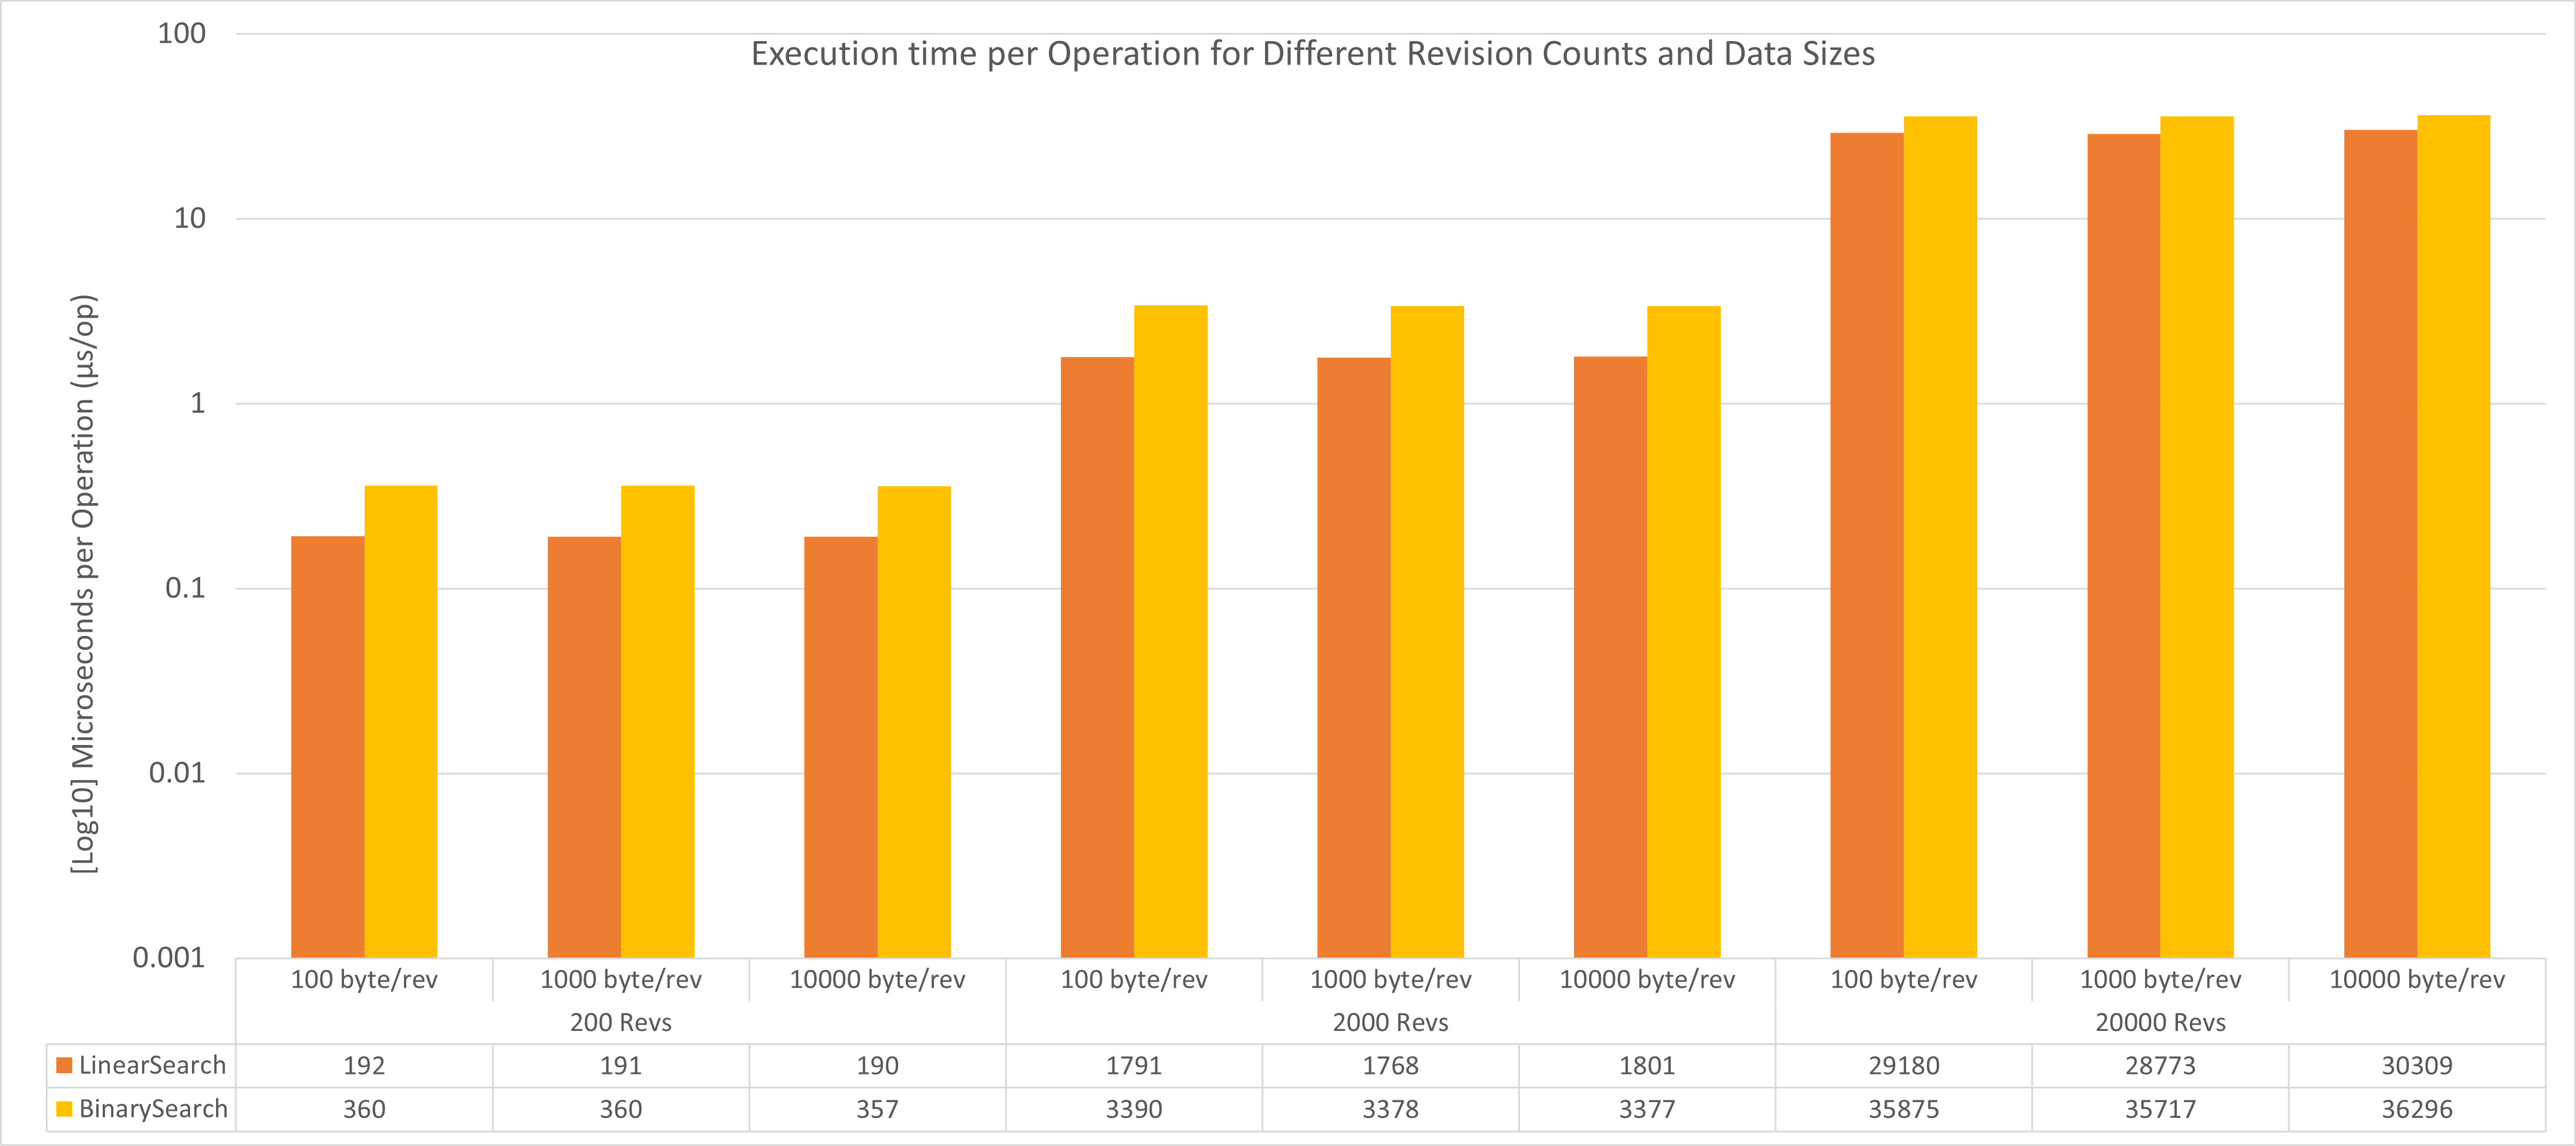
\includegraphics[width=1\linewidth]{charts/LS&BS_ns_all.png}
        \caption{Execution Time}
        \label{fig:linear-search-binary-search-execution-time}
    \end{subfigure}

    \caption{Execution time for the Linear Search and Binary Search algorithms.}
    \label{fig:linear-search-binary-search-performance-metrics}
\end{figure}

\paragraph{Execution Time}
The execution time for the \lstinline{Linear Search} and \lstinline{Binary Search} algorithms is very similar across all data sizes. This is likely due to the fact that the \lstinline{Linear Search} algorithm is iterating through the entire data set, regardless of the data size. The \lstinline{Binary Search} algorithm is also iterating through the entire data set, but it is doing so in a more efficient manner. The \lstinline{Binary Search} algorithm is able to skip over half of the data set with each iteration, therefore it should prove to be more efficient than the \lstinline{Linear Search} algorithm, so it is unclear why the execution time is so similar or even worse in some cases.

\paragraph{Memory Usage}
The \lstinline{Linear Search} and \lstinline{Binary Search} algorithms both have a memory usage of 0 bytes per operation. This is because the algorithms are not allocating any memory during their execution.

\paragraph{Memory Allocation}
The \lstinline{Linear Search} and \lstinline{Binary Search} algorithms both have a memory allocation of 0 allocations per operation. This is because the algorithms are not allocating any memory during their execution.

\newpage

\begin{table}[H]
    \centering
    \begin{tabular}{|r|r|r|r|r|}
        \hline
        \multicolumn{1}{|c|}{\textbf{num\_revisions}} & \multicolumn{1}{c|}{\textbf{data\_size}} & \multicolumn{1}{c|}{\textbf{ns\_per\_op}} & \multicolumn{1}{c|}{\textbf{bytes\_per\_op}} & \multicolumn{1}{c|}{\textbf{allocs\_per\_op}} \\ \hline
        200 Revs                                      & 100 byte/rev                             & 8670                                      & 4248                                         & 15                                            \\ \hline
        200 Revs                                      & 1000 byte/rev                            & 8698                                      & 4264                                         & 15                                            \\ \hline
        200 Revs                                      & 10000 byte/rev                           & 8863                                      & 4259                                         & 15                                            \\ \hline
        2000 Revs                                     & 100 byte/rev                             & 91438                                     & 47907                                        & 68                                            \\ \hline
        2000 Revs                                     & 1000 byte/rev                            & 93066                                     & 47916                                        & 68                                            \\ \hline
        2000 Revs                                     & 10000 byte/rev                           & 85277                                     & 47833                                        & 68                                            \\ \hline
        20000 Revs                                    & 100 byte/rev                             & 1092353                                   & 474162                                       & 360                                           \\ \hline
        20000 Revs                                    & 1000 byte/rev                            & 886706                                    & 475409                                       & 361                                           \\ \hline
        20000 Revs                                    & 10000 byte/rev                           & 839202                                    & 476277                                       & 361                                           \\ \hline
    \end{tabular}
    \caption{Performance metrics for the Depth First Search algorithm.}
    \label{tab:depth-first-search-benchmark-results}
\end{table}
\begin{table}[h]
    \centering
    \begin{tabular}{|r|r|r|r|r|}
        \hline
        \multicolumn{1}{|c|}{\textbf{num\_revisions}} & \multicolumn{1}{c|}{\textbf{data\_size}} & \multicolumn{1}{c|}{\textbf{ns\_per\_op}} & \multicolumn{1}{c|}{\textbf{bytes\_per\_op}} & \multicolumn{1}{c|}{\textbf{allocs\_per\_op}} \\ \hline
        200 Revs                                      & 100 byte/rev                             & 14648                                     & 5044                                         & 114                                           \\ \hline
        200 Revs                                      & 1000 byte/rev                            & 14538                                     & 5052                                         & 115                                           \\ \hline
        200 Revs                                      & 10000 byte/rev                           & 14817                                     & 5058                                         & 115                                           \\ \hline
        2000 Revs                                     & 100 byte/rev                             & 146733                                    & 55869                                        & 1066                                          \\ \hline
        2000 Revs                                     & 1000 byte/rev                            & 148890                                    & 55971                                        & 1067                                          \\ \hline
        2000 Revs                                     & 10000 byte/rev                           & 141562                                    & 55981                                        & 1068                                          \\ \hline
        20000 Revs                                    & 100 byte/rev                             & 1479317                                   & 561308                                       & 10478                                         \\ \hline
        20000 Revs                                    & 1000 byte/rev                            & 1405637                                   & 550430                                       & 10323                                         \\ \hline
        20000 Revs                                    & 10000 byte/rev                           & 1394722                                   & 556945                                       & 10399                                         \\ \hline
    \end{tabular}
    \caption{Performance metrics for the Breadth First Search algorithm.}
    \label{tab:breadth-first-search-benchmark-results}
\end{table}
% \newpage

\begin{figure}[H]
    \centering
    \begin{subfigure}[b]{0.75\textwidth}
        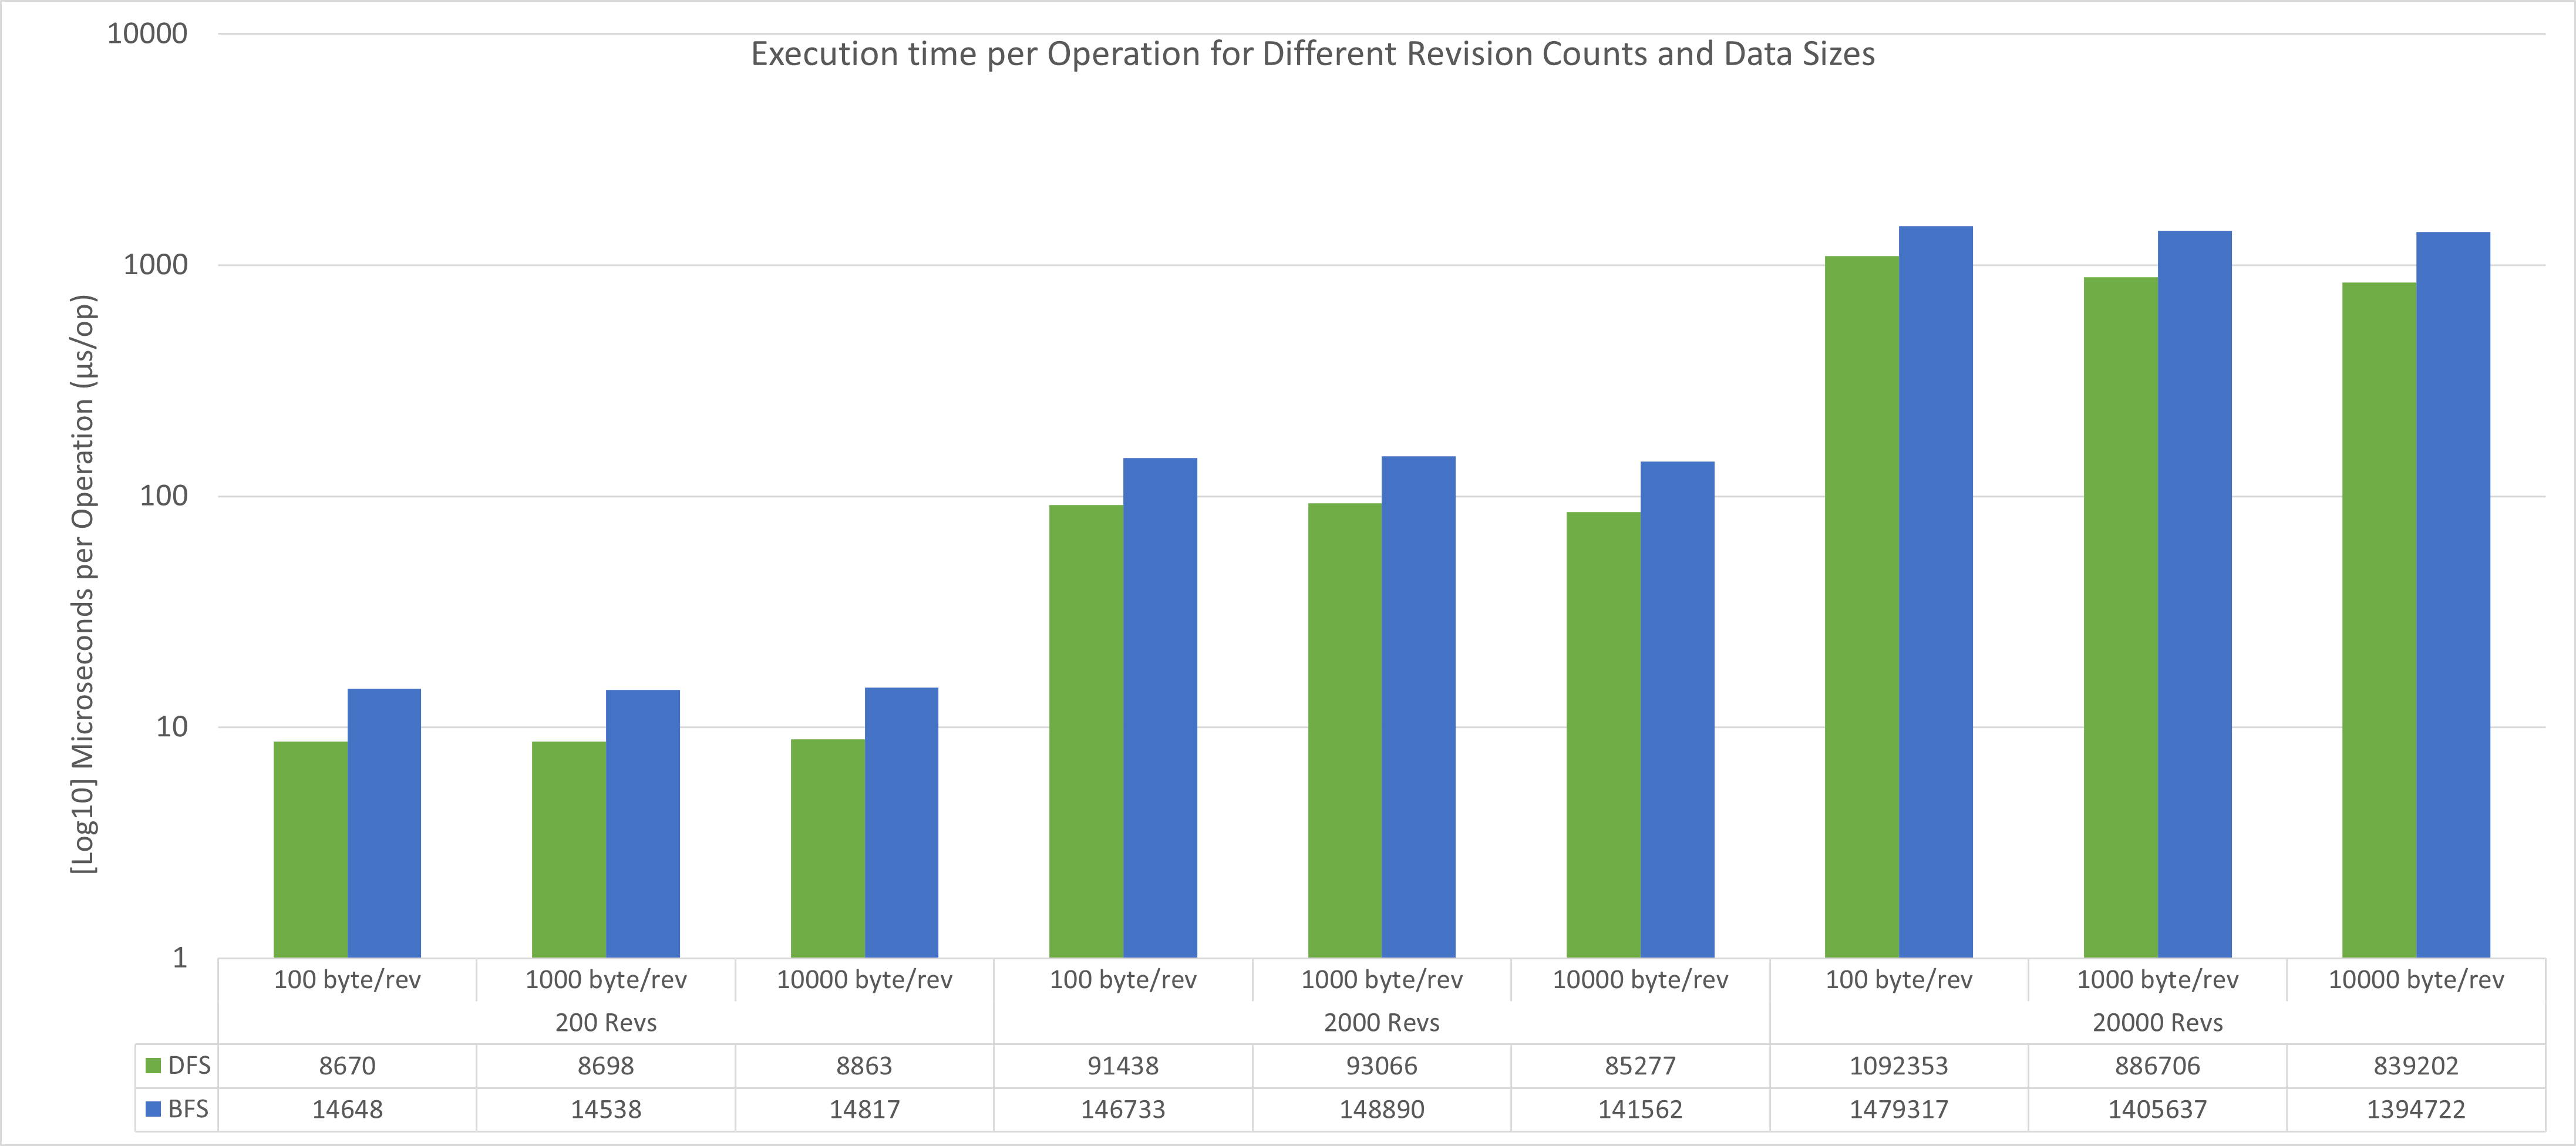
\includegraphics[width=1\linewidth]{charts/DFS&BFS_ns_all.png}
        \caption{Execution Time}
        \label{fig:depth-first-search-breadth-first-search-execution-time}
    \end{subfigure}

    \begin{subfigure}[b]{0.75\textwidth}
        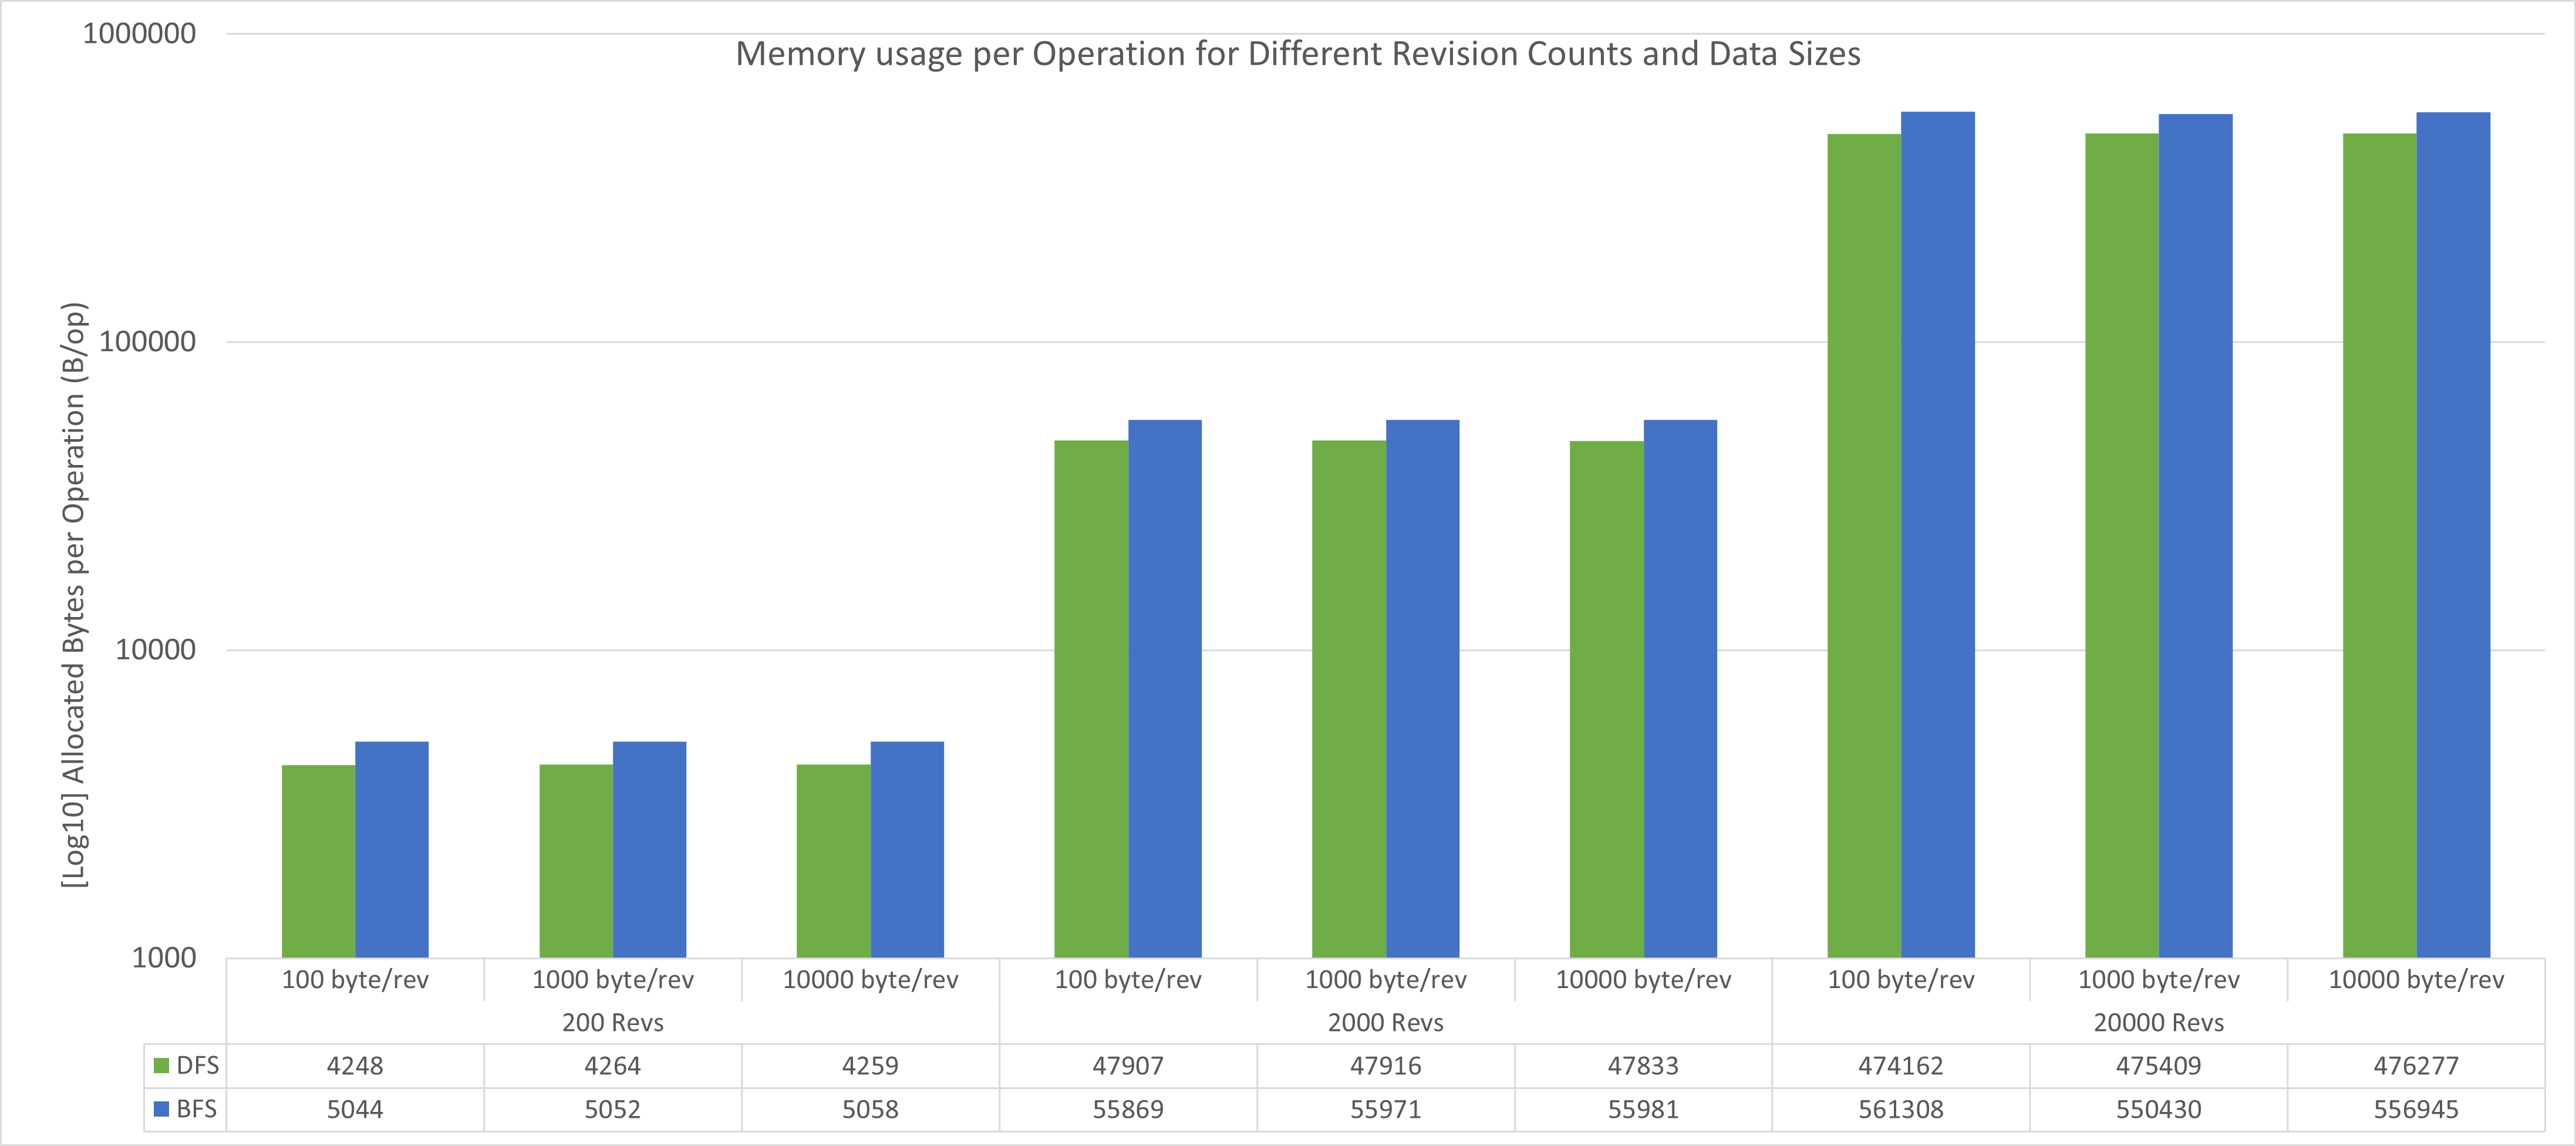
\includegraphics[width=1\linewidth]{charts/DFS&BFS_bytes_all.png}
        \caption{Memory Usage}
        \label{fig:depth-first-search-breadth-first-search-memory-usage}
    \end{subfigure}

    \begin{subfigure}[b]{0.75\textwidth}
        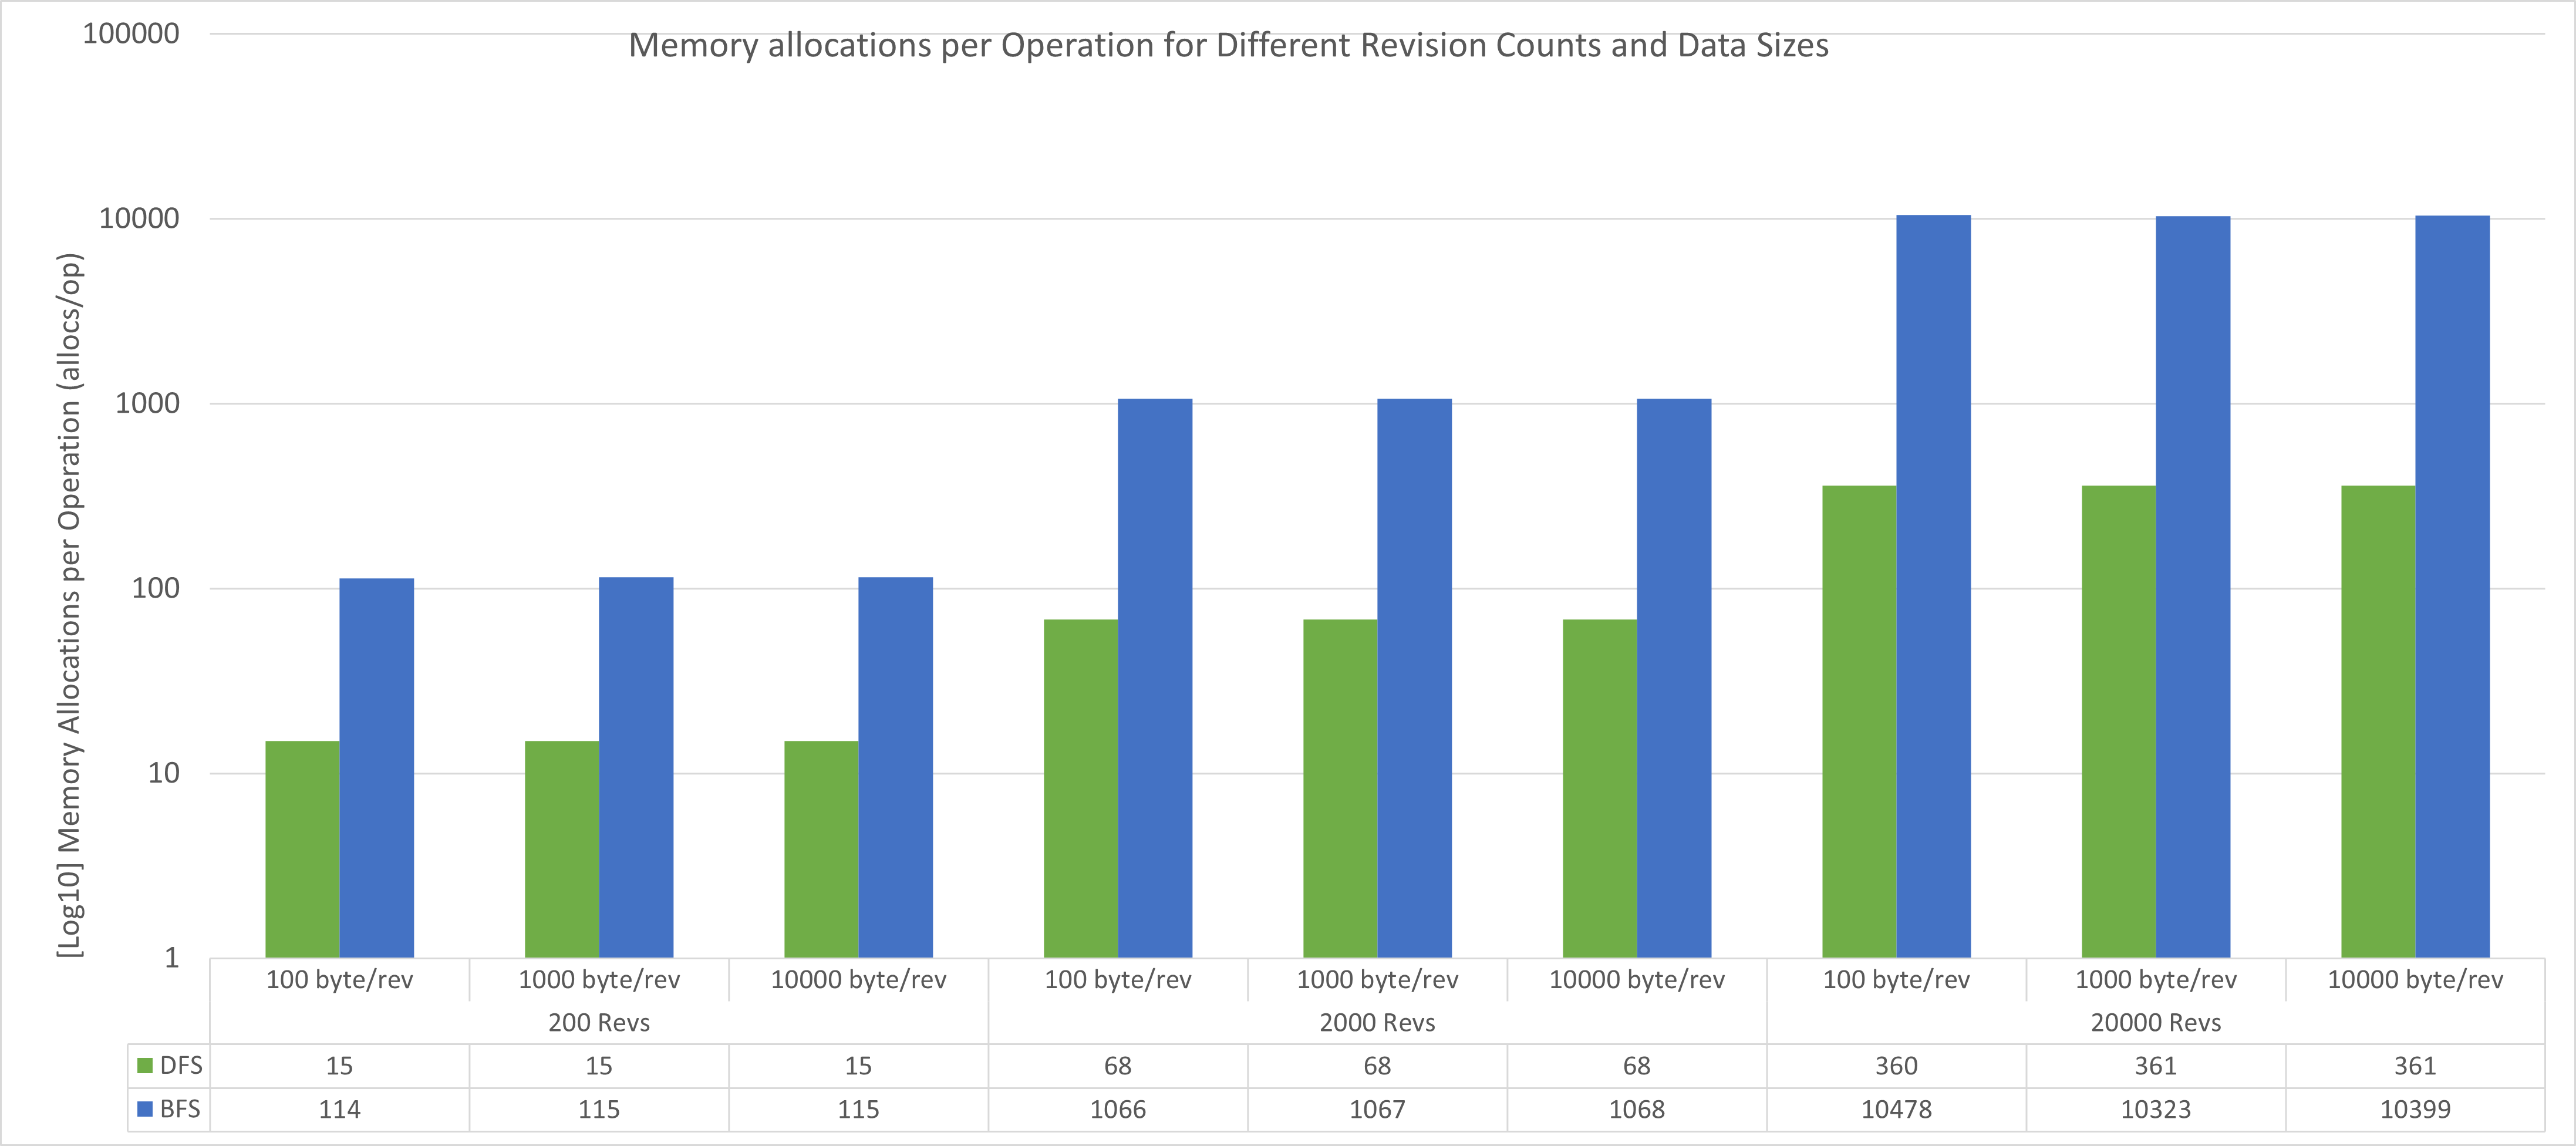
\includegraphics[width=1\linewidth]{charts/DFS&BFS_allocs_all.png}
        \caption{Memory Allocations}
        \label{fig:depth-first-search-breadth-first-search-memory-allocations}
    \end{subfigure}

    \caption{Performance metrics for the Depth First Search and Breadth First Search algorithms.}
    \label{fig:depth-first-search-breadth-first-search-performance-metrics}
\end{figure}

\paragraph{Execution Time}
The execution time gap between the \lstinline{Depth First Search} and \lstinline{Breadth First Search} algorithms stays relatively similar as the number of revisions increases. The \lstinline{Depth First Search} algorithm is consistently faster than the \lstinline{Breadth First Search} algorithm.

\paragraph{Memory Usage}
The memory usage gap between the \lstinline{Depth First Search} and \lstinline{Breadth First Search} algorithms stays relatively similar as the number of revisions increases. The \lstinline{Depth First Search} algorithm consistently uses less memory than the \lstinline{Breadth First Search} algorithm.

\paragraph{Memory Allocations}
The memory allocation gap between the \lstinline{Depth First Search} and \lstinline{Breadth First Search} algorithms is much wider than the execution time and memory usage gaps. The \lstinline{Depth First Search} algorithm consistently allocates much less memory than the \lstinline{Breadth First Search} algorithm.

\newpage

\subsection{Diff Algorithms}

\begin{table}[h]
    \centering
    \begin{tabular}{|l|r|r|r|}
        \hline
        \multicolumn{1}{|c|}{\textbf{test\_case}} & \multicolumn{1}{c|}{\textbf{ns\_per\_op}} & \multicolumn{1}{c|}{\textbf{bytes\_per\_op}} & \multicolumn{1}{c|}{\textbf{allocs\_per\_op}} \\ \hline
        Small                                     & 2231                                      & 2008                                         & 36                                            \\ \hline
        Large                                     & 161544303                                 & 74748939                                     & 22243                                         \\ \hline
        Extreme                                   & 159264376                                 & 74717878                                     & 21757                                         \\ \hline
    \end{tabular}
    \caption{Performance metrics for the Myers Diff algorithm.}
    \label{tab:myers-diff-benchmark-results}
\end{table}
\begin{table}[h]
    \centering
    \begin{tabular}{|l|r|r|r|}
        \hline
        \multicolumn{1}{|c|}{\textbf{test\_case}} & \multicolumn{1}{c|}{\textbf{ns\_per\_op}} & \multicolumn{1}{c|}{\textbf{bytes\_per\_op}} & \multicolumn{1}{c|}{\textbf{allocs\_per\_op}} \\ \hline
        Small                                     & 3987                                      & 3081                                         & 64                                            \\ \hline
        Large                                     & 344500                                    & 378884                                       & 6071                                          \\ \hline
        Extreme                                   & 123503                                    & 204634                                       & 2047                                          \\ \hline
    \end{tabular}
    \caption{Performance metrics for the Patience Diff algorithm.}
    \label{tab:patience-diff-benchmark-results}
\end{table}

\begin{figure}[h]
    \centering
    \begin{subfigure}[b]{0.75\textwidth}
        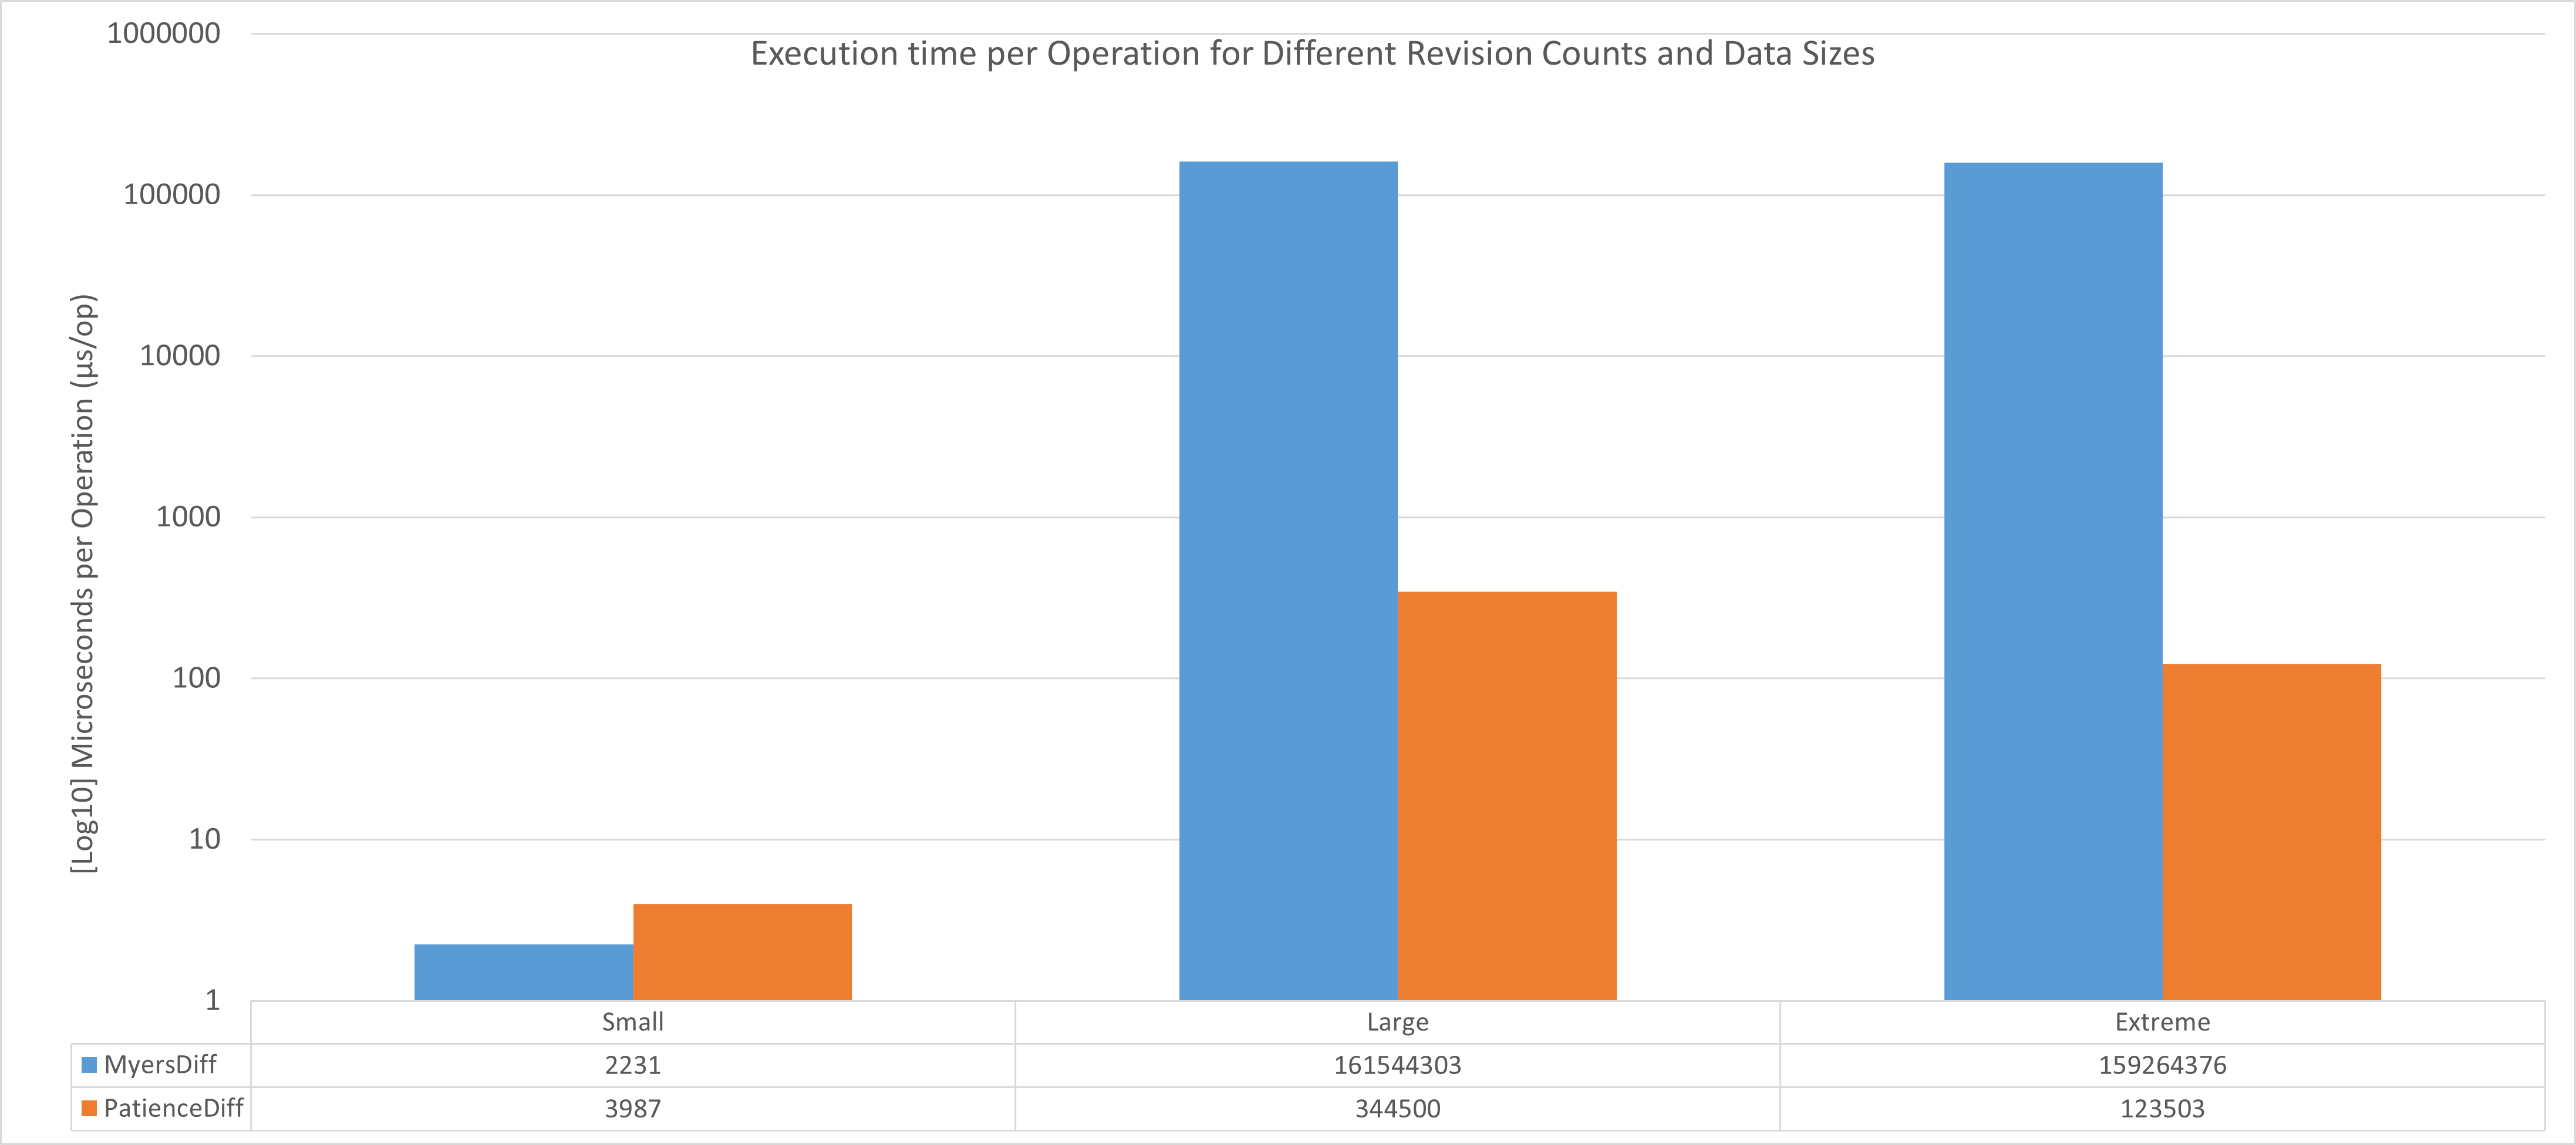
\includegraphics[width=1\linewidth]{charts/diff_ns_all.png}
        \caption{Execution Time}
        \label{fig:myers-diff-patience-diff-execution-time}
    \end{subfigure}

    \begin{subfigure}[b]{0.75\textwidth}
        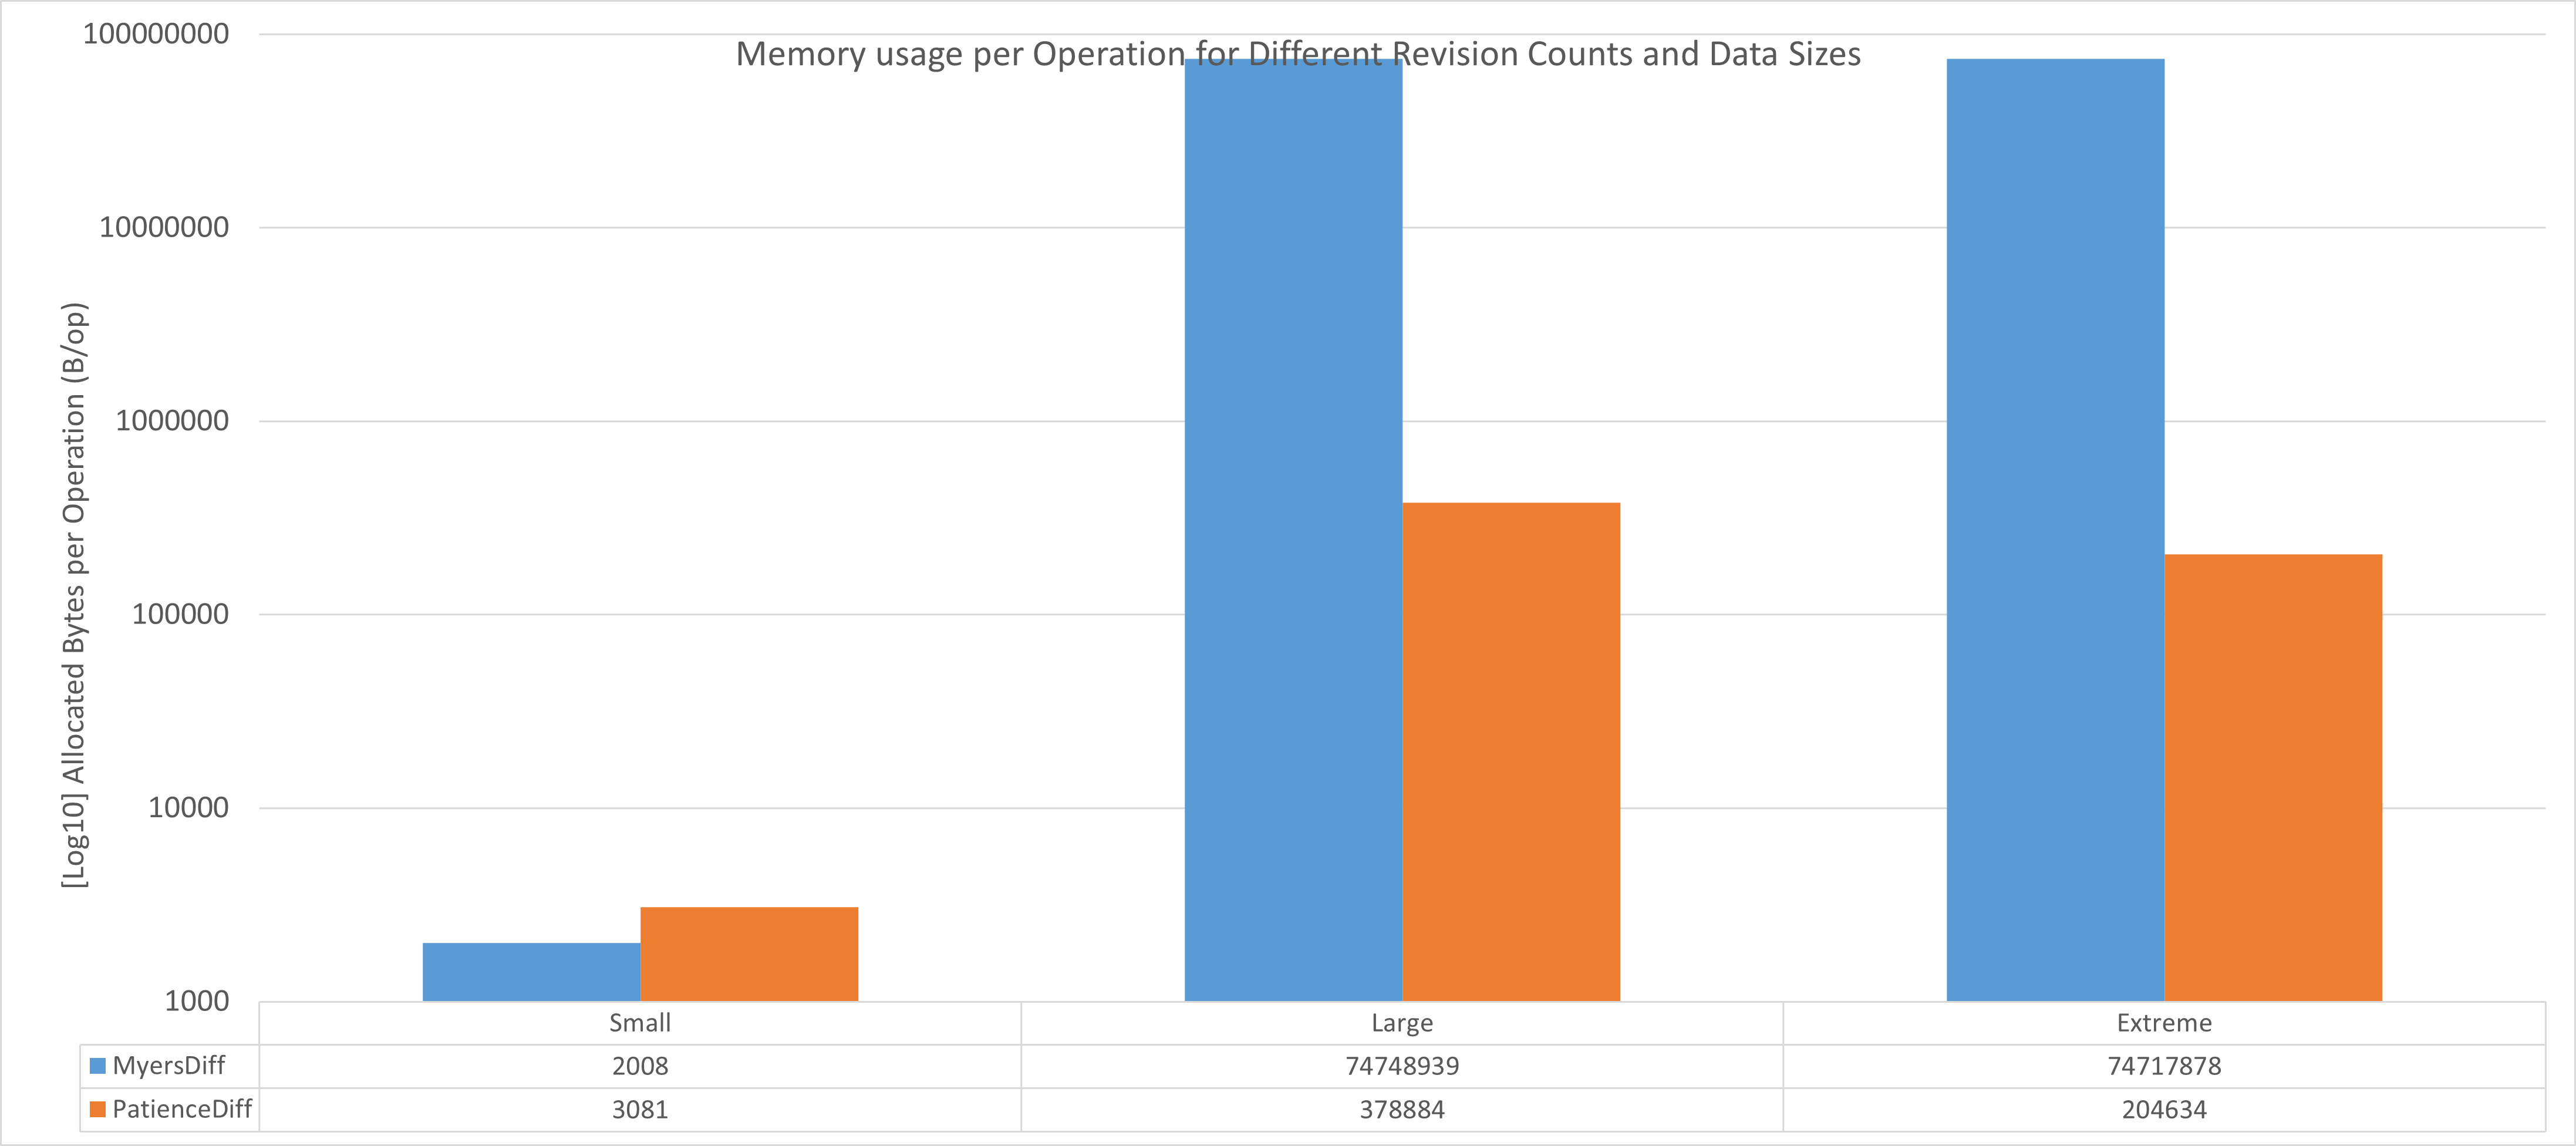
\includegraphics[width=1\linewidth]{charts/diff_bytes_all.png}
        \caption{Memory Usage}
        \label{fig:myers-diff-patience-diff-memory-usage}
    \end{subfigure}

    \begin{subfigure}[b]{0.75\textwidth}
        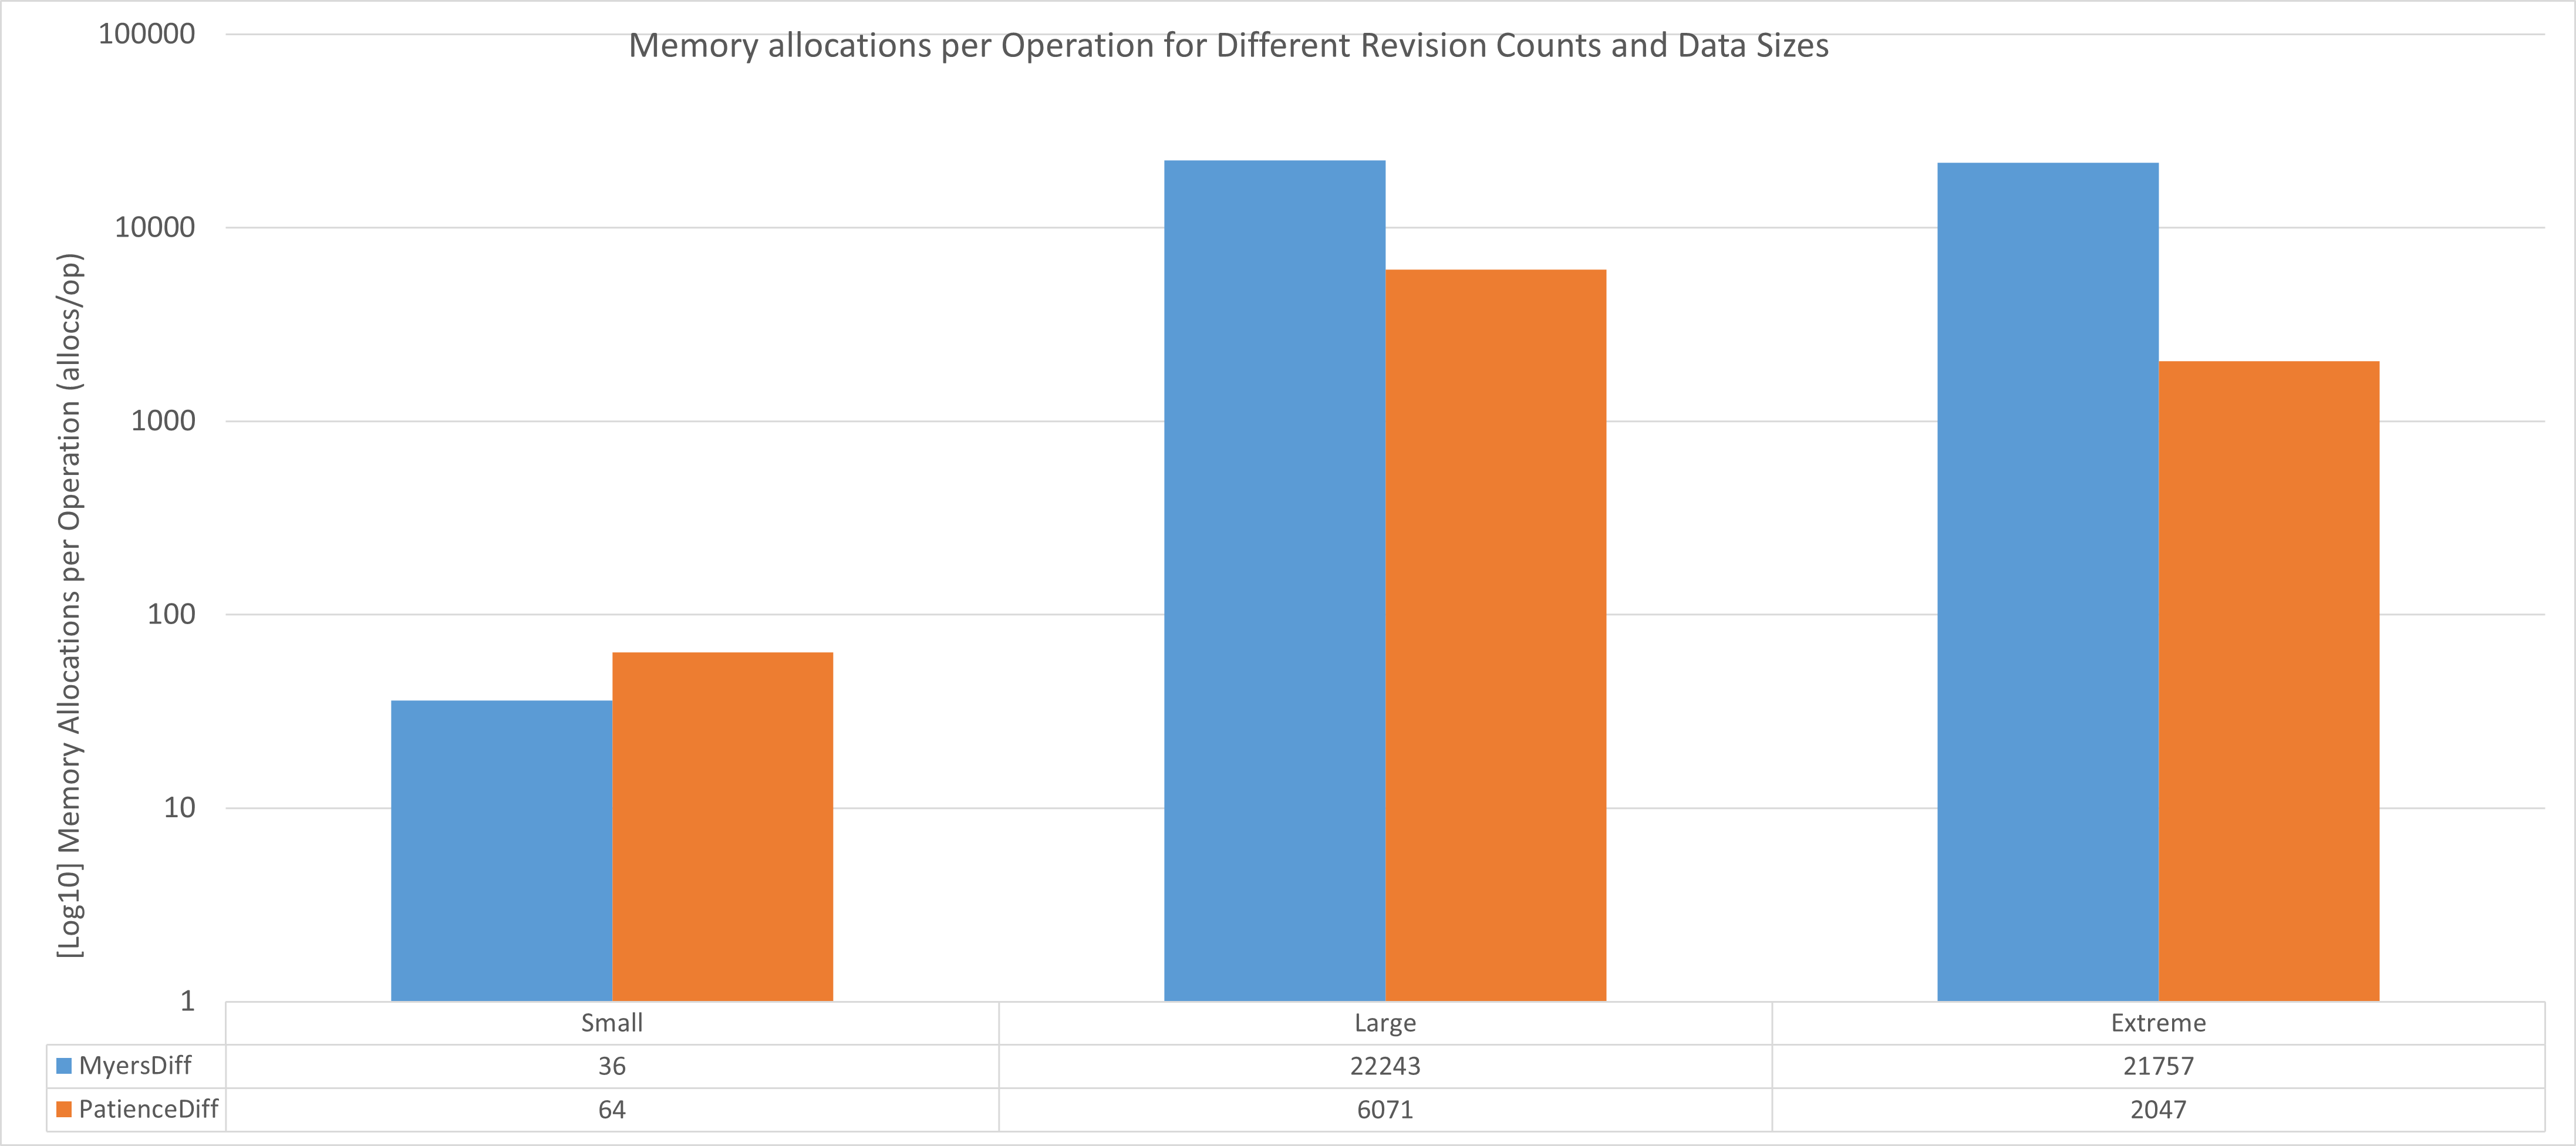
\includegraphics[width=1\linewidth]{charts/diff_allocs_all.png}
        \caption{Memory Allocations}
        \label{fig:myers-diff-patience-diff-memory-allocations}
    \end{subfigure}

    \caption{Performance metrics for the Myers Diff and Patience Diff algorithms.}
    \label{fig:myers-diff-patience-diff-performance-metrics}
\end{figure}


\newpage
\chapter{Conclusion} % (4-6 pages)
\label{chap:conclusion}

\section{Challenges}
\noindent
Several challenges were faced during the course of this project, the main ones being:

Firstly, it was challenging to find information on the technical aspects of existing Version Control Systems, especially the earlier generations of Version Control Systems. The lack of information on these technical aspects made it difficult to understand how the systems were implemented and what underlying data structures and algorithms were used.
\smallskip

Secondly, it was challenging to identify which data structures and algorithms would provide meaningful points of comparison. The vast number of data structures and algorithms made it challenging to select a suitable set for evaluation. The selected data structures and algorithms had to be representative of those used in real-world Version Control Systems and provide a basis for meaningful comparison.
\smallskip

Thirdly, I had to learn the Go programming language's built-in benchmarking package, which they were initially unfamiliar with. The learning curve for this package was steep, and it took time to understand how to use it effectively for the purposes of this research project.
\smallskip

Finally, it was challenging to design automated benchmarks using mock data that were still representative of real-world use. The mock data had to be generated in a way that was realistic and representative of the data used in real-world Version Control Systems. This required careful consideration of the different types of data used in Version Control Systems and how they could be represented in the mock data.

\section{Future Work}
\noindent
One possible area for future work is implementing a fully functional Version Control System to obtain the most realistic data for benchmarking. The fully functional Version Control System would allow for more realistic testing and benchmarking of the data structures and algorithms and provide insight into their performance under real-world usage scenarios.
Other areas for future work are evaluating other data structures and algorithms not considered in this research project and developing more advanced benchmarking techniques than those used in this project.
\newpage

% Terminology section
% ==============================================================================
% TODO: Add terminology
% ==============================================================================

% Figures section
% ==============================================================================
\listoffigures
\addcontentsline{toc}{chapter}{List of Figures}
\newpage
% ==============================================================================

% Tables section
% ==============================================================================
\listoftables
\addcontentsline{toc}{chapter}{List of Tables}
\newpage
% ==============================================================================

% Bibliography section
% ==============================================================================
\bibliographystyle{ieeetr}
\bibliography{../bibliography/vcs_info}
\addcontentsline{toc}{chapter}{Bibliography}
% ==============================================================================

\end{document}
